% A compiler avec xelatex
\documentclass[11pt]{article}

\usepackage[utf8]{inputenc}
\usepackage[french]{babel}
\hyphenation{person-nage person-nages-joueurs}

\usepackage{comment}

% Pour inclure la page de garde
\usepackage{pdfpages}

%geometry of the page
%TODO Enlever le cadre une fois le document terminé
\usepackage[vmargin=0.6in,hmargin=1in]{geometry}
%\usepackage[vmargin=0.6in,hmargin=1in,showframe]{geometry}

\setlength{\parindent}{1cm}

%========================================= FONTS
\usepackage{fontspec}


%TODO désactiver la police Méga
% Test de police Méga
%\newcommand{\MEGA}{\fontsize{110}{-30}\fontspec{Mega:style=JDR-ORey}\selectfont}


% Police de caractères OD&D Saloon Girl Inline
%\newcommand{\ODDtitlefont}{\fontsize{38}{40}\fontspec{QuentinCaps}\selectfont}
\newcommand{\ODDtitlefont}{\fontsize{60}{40}\fontspec{Saloon Girl Inline}\selectfont}

% Police de caractères OD&D OPTIChisel-Normal:style=Regular
\newcommand{\ODDtitlebisfont}{\fontsize{52}{70}\fontspec{OPTIChisel-Normal:style=Regular}\selectfont}
\newcommand{\ODDsectionfont}{\fontsize{42}{50}\fontspec{OPTIChisel-Normal:style=Regular}\selectfont}

%TODO Choisir pour le PC 32 ou 64 bits
% Pour le PC 64 bits
\newcommand{\ODDtimes}{\fontspec{Times New Roman}\selectfont}
% Pour le PC 32 bits
%\newcommand{\ODDtimes}{\fontspec{Linux Libertine O}\selectfont}

%- \usepackage{xcolor}
\usepackage{titlesec}
\defaultfontfeatures{Ligatures=TeX}
% Set sans serif font to Calibri
%- \setsansfont{Calibri}

% Set main font
\setmainfont{Futura Std}

\usepackage{hyperref}
\hypersetup{
pdfauthor={Olivier Rey},
pdftitle={OD\&D -- Eldritch Wizardry -- Pouvoirs psioniques},
pdfkeywords={jdr,D\&D,0e,ODD,Gygax,Blume,TTRPG},
pdfsubject={OD\&D -- Eldritch Wizardry -- Pouvoirs psioniques},
pdfcreator={TexStudio for xetex},
pdflang={French},
colorlinks=true,
linkcolor={teal},
urlcolor={teal},
bookmarksopen=true,
bookmarksopenlevel=2,
}

% Define light and dark Microsoft blue colours
%- \definecolor{MSBlue}{rgb}{.204,.353,.541}
%- \definecolor{MSLightBlue}{rgb}{.31,.506,.741}
% Define a new fontfamily for the subsubsection font
% Don't use \fontspec directly to change the font
%- \newfontfamily\subsubsectionfont[Color=MSLightBlue]{Times New Roman}
% Set formats for each heading level
%\titleformat*{\section}{\normalfont\fontsize{12}\ttfamily{QuentinCaps}}

%\titleformat{\section}{\fontspec{QuentinCaps}\selectfont}{\thesection}{1em}{}

\titleformat{\section}{\centering\ODDsectionfont}{\thesection}{1em}{}
\titleformat{\subsection}{\large\bfseries}{\thesubsection}{1em}{}
\titleformat{\subsubsection}{\large\bfseries}{\thesubsubsection}{1em}{}


%- \titleformat*{\subsection}{\large\bfseries\sffamily\color{MSLightBlue}}
%- \titleformat*{\subsubsection}{\itshape\subsubsectionfont}

% pour le (R)
\usepackage{fontspec}

% Pour les images
\usepackage{graphicx}
\graphicspath{{./yed/}{./images/}{./maps/}}

% Array stretch pour avoir un peu plus de vertical spacing dans les tabular
\usepackage{tabularx}
\renewcommand{\arraystretch}{1.2}
\usepackage{multirow}

% Place les footnotes en bas et supprimer l'indentation dans la footnote
\usepackage[bottom]{footmisc}

% Pur résoudre les problèmes de underline avec la ligne qui varie en hauteur
\newcommand{\uline}[1]{\underline{\smash{#1}\vphantom{T}}\vphantom{#1}}

% Macro pour réduire l'espace sous le titre
\newcommand{\myunderline}[1]{\underline{\smash{#1}}}

% Renommer la table des matières en Index
\addto\captionsfrench{% Replace "english" with the language you use
  \renewcommand{\contentsname}%
    {Index}%
}

% En fait le \label dans le texte ne fonctionne pas toujours avec \pageref
% Cette commande permet de fixer le sujet
\newcommand\pagelabel{\phantomsection\label}


%++++++++++++++++++++++++++++++++++++++++++++++++++++++++++++++++++++++++++
%                               DOCUMENT
%++++++++++++++++++++++++++++++++++++++++++++++++++++++++++++++++++++++++++
\begin{document}

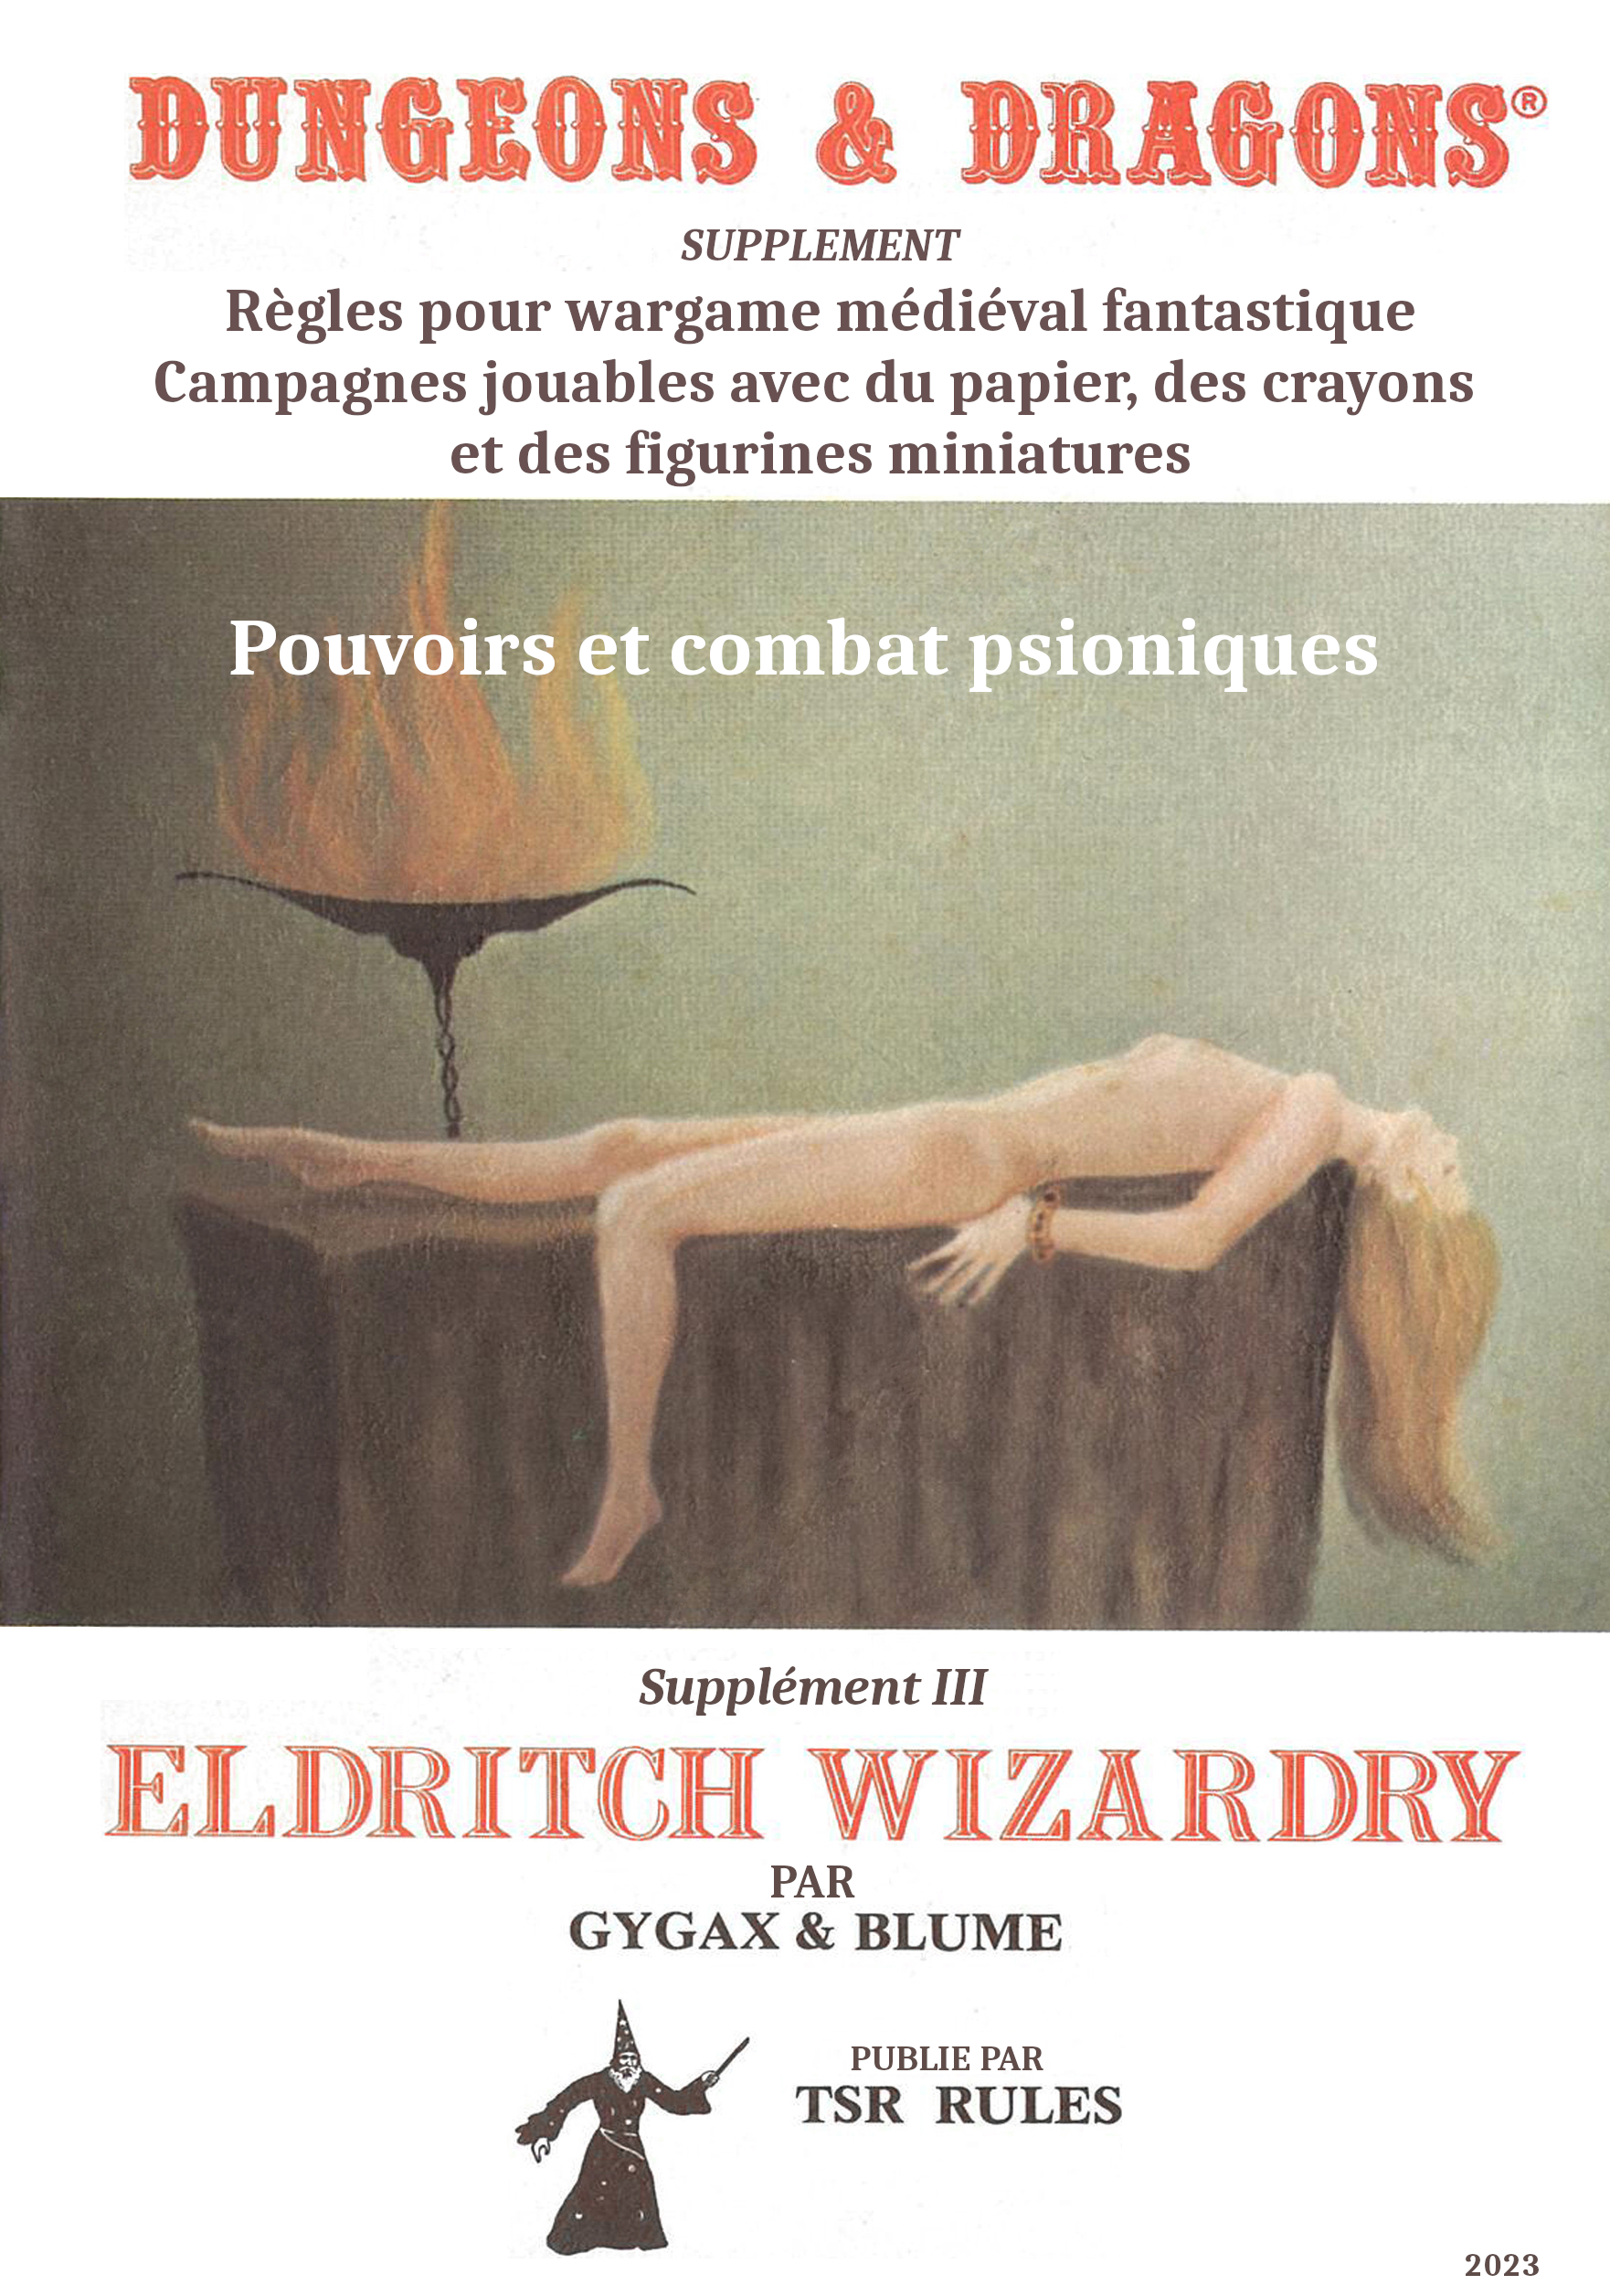
\includepdf[scale=0.9]{pagedegarde.pdf}
\newpage

{\color{white}-}

\newpage

\thispagestyle{empty}
\begin{center}
{\Huge \ODDtitlefont{DONJONS \& DRAGONS}}{\normalsize \textsuperscript{\sffamily\textregistered}}

\vspace{1.8cm}

{\Large \textbf{Supplément III}}

\vspace{1.3cm}

{\Huge \ODDtitlebisfont{ELDRITCH}}

\vspace{0.3cm}

{\Huge \ODDtitlebisfont{WIZARDRY}}

\vspace{2.0cm}

{\Large \textbf{MAGIE ANCIENNE ET PUISSANTE}}

\vspace{1cm}

{\large PAR

\vspace{0.1cm}

GARY GYGAX \& BRIAN BLUME

\vspace{3cm}

Remerciements spéciaux à l'aîné Steve Marsh, Dennis Sustare (le Super Druide),

Jim Ward \& Tim Kask pour leurs suggestions et contributions !

\vspace{0.8cm}

Illustrations de Dave Sutherland, Tracy Lesch \& Gary Kwapisz

Couverture par Deborah Larson}

\vspace{1.3cm}

\textbf{\ODDtimes{2023}}

\vspace{0.5cm}

\ODDtimes{\textbf{\textcopyright\ 1976 - TSR GAMES}

\textbf{9\textsuperscript{ème} impression, novembre 1979}

\textbf{Imprimé aux U.S.A}}
\end{center}

\vfill

{\small \noindent LES QUESTIONS SUR LES REGLES DOIVENT ETRE ACCOMPAGNEES D'UNE ENVELOPPE RETOUR TIMBREE ET ENVOYEES A TACTICAL STUDIES RULES, POB 756, LAKE GENEVA, WISCONSIN 53147}


\newpage
%====================================================
{\color{white}a}

\vfill

\noindent{\scriptsize \textit{Ce fascicule est une adaptation par Rouboudou (\href{https://rouboudou.itch.io}{rouboudou.itch.io}) de la partie pouvoirs psioniques du livret original. Cette adaptation est une œuvre de fan. Elle est soumise à la licence OGL que vous trouverez page \pageref{OGL}.}}

\newpage

\phantomsection\section*{Préface}
\addcontentsline{toc}{section}{Préface}

Le livre que vous tenez maintenant dans vos mains présente de nouvelles dimensions à un système de jeu déjà fascinant. Il s'agit du troisième supplément à DONJONS \& DRAGONS, produit comme conséquence à une demande toujours croissante de matériel nouveau.

Ce livre présente aussi une nouvelle mode dans l'art subtil d'être Maître de Donjon. Fidèle à sa conception d'origine, D\&D n'était limité dans son périmètre que par l'imagination et la dévotion des Maîtres de Donjons où qu'ils soient. Les suppléments ont répondu au besoin d'idées nouvelles et de mécanismes de simulation additionnels. Mais progressivement, D\&D a perdu un peu de sa saveur, et a commencé à devenir prévisible. Cela était dû à la prolifération d'ensembles de règles ; alors que c'était très bien pour nous en tant de compagnie, c'était compliqué pour le MD. Quand tous les joueurs avaient toutes les règles en face d'eux, il devenait presque qu'impossible de les séduire à affronter le danger ou les pièges.

Le nouveau concept innovant présenté dans ces pages devrait faire long feu en réintroduisant un peu de mystère, d'incertitude et de danger, qui refont de D\&D le défi sans équivalent qu'il a toujours été. La légende retrouve sa magie inestimable originale. On ne verra plus d'aventurier imprudent descendre dans un donjon, trouver quelque chose et savoir immédiatement ce que cela fait et comment cela fonctionne. De même, les joueurs ne pourront plus envoyer un de leurs infortunés serviteurs à une mort précoce en le forçant à expérimenter à la place de son maître.

L'introduction du combat psionique est destiné à revivifier des parties devenues stagnantes. Il ouvre de nouvelles possibilités à la fois aux joueurs et au MD, tout en intégrant un des sujets favoris des auteurs de science-fiction et de fantastique : les pouvoirs inconnus de l'esprit.

Comme pour les deux précédents suppléments, le matériel contenu dans ce livret propose le même format que les trois livrets originaux de D\&D. Les corrections et les ajouts sont indiqués dans le texte de sorte qu'ils puissent être intégrés facilement dans les règles originales.

Comme vous pourrez le noter sur la page de titre, ce supplément est le fruit de plusieurs contributeurs. Telle est la nature de la chose que vous tenez entre vos mains. D\&D a été conçu pour être un jeu libre, lié aux règles de manière souple. Nous pensons que ELDRITCH WIZARDRY favorise les principes originaux de danger, d'excitation et d'incertitude. Que vous réussissiez toujours vos jets de sauvegarde.

\vspace{1cm}

\noindent Timothy J. Kask

\noindent TSR Publications Editor

\noindent Lake Geneva, Wisconsin

\noindent 23 avril 1976

\newpage

\phantomsection\section*{Introduction}
\addcontentsline{toc}{section}{Introduction}

Le terme anglais \texttt{psionic} a été utilisé la première fois en 1951 dans une nouvelle de science-fiction écrite par Jack Williamson, \texttt{The Greatest Invention}, publié dans le magazine \texttt{Astounding Science Fiction}. Il est la compression de deux termes : \texttt{psi} dans le sens de phénomène psychique, et \texttt{electronics}. \texttt{Psionics} devient un terme décrivant la discipline qui étudie les phénomènes psychiques avec les moyens de l'ingénierie moderne de l'époque, soit l'électronique. Malgré la promotion de personnes comme John W. Campbell, le terme restera utilisé uniquement dans le monde de la science-fiction, avant d'être intégré dans le monde des jeux de rôles.

La version originale de Donjons \& Dragons, dite OD\&D, est publiée en 1974 sous la forme de trois livrets à la couverture marron. On trouve dans le premier livret, \texttt{Men \& Magic}, un certain nombre de sorts ressemblant à des pouvoirs psychiques, et dans le deuxième, \texttt{Monsters \& Treasures}, les premières références à des pouvoirs psychiques, dans la section traitant des épées magiques. A l'époque, le terme \texttt{psionic} n'est pas utilisé.

En 1976, dans le troisième supplément \texttt{Eldritch Wizardry} cosigné par Gary Gygax et Brian Blume, publié après \texttt{Greyhawk} et \texttt{Blackmoor}, les pouvoirs psychiques arrivent dans le monde des personnages-joueurs et des personnages-non-joueurs. Les règles sont présentées de manière assez chaotique, ce qui générera vite la réputation d'un système injouable dans le monde des joueurs. Derrière la juste critique sur la présentation, beaucoup de joueurs semblent avoir rejeté le supplément en raison du fait même de proposer, en extension à un jeu médiéval-fantastique, une gestion des pouvoirs mentaux, habituellement présents dans les univers de science-fiction.

Nous proposons ici une double présentation des règles psioniques du supplément \texttt{Eldritch Wizardry}, supplément qui contient d'autres choses non traduites en ces pages (notamment le Druide, des monstres, etc.) :

\begin{itemize}
\item La première partie propose une traduction complète, la plus fidèle possible, des règles originales relatives aux pouvoirs psioniques. En effet, le texte original étant touffu, nous avons veillé à traduire le plus fidèlement possible ses nuances (ce qui donne un style parfois un peu lourd, proche du style original). Dans cette partie, nous avons tenté de respecter l'aspect original des règles (polices, alignements, etc.).
\item Cette première partie a été, en quelque sorte, \og augmentée \fg{} : en effet, \texttt{Eldritch Wizardry} étant une extension de OD\&D, le texte pointe vers les références présentes dans les livrets précédents ; nous avons extrait ces références pour en proposer une traduction au sein même de ce livre, de sorte que cette compilation devrait se suffire à elle-même et ne pas nécessiter d'ouvrir les ouvrages précédents de la série.
\item La seconde partie propose une réorganisation complète de ces règles visant à les présenter de manière plus claire et plus logique ; nous espérons que nous aurons été à la hauteur du chantier, plus complexe qu'il n'y paraissait au départ.
\end{itemize}

La consultation de certains sites américains a été nécessaire pour s'assurer de la bonne compréhension de certaines règles ambiguës qui, encore aujourd'hui, provoquent des commentaires et des incompréhensions.

Une fois éclairci, le système se montre très intéressant, non seulement parce qu'il est très \og gygaxien \fg{} (on le voit notamment au travers de l'utilisation de règles gigognes), mais aussi parce qu'il est le premier système complet de pouvoirs psychiques, très différent de la magie de OD\&D, et qu'il inspirera beaucoup d'autres systèmes de pouvoirs basés sur la consommation de points d'énergie psionique.

\vspace{0.7cm}

\noindent Rouboudou

\noindent https://orey.github.io/blog

\noindent Août 2023

\newpage

%\phantomsection\section*{Index}
%\addcontentsline{toc}{section}{Index}

\phantomsection\tableofcontents
\addcontentsline{toc}{section}{Index}

%+=+=+=+=+=+=+=+=+=+=+=+=+=+=+=+=+=+=+=+=+=+=+=+=+=+=+=+=+=+=+=+=+=+=+=+= PART
%+=+=+=+=+=+=+=+=+=+=+=+=+=+=+=+=+=+=+=+=+=+=+=+=+=+=+=+=+=+=+=+=+=+=+=+= PART
%+=+=+=+=+=+=+=+=+=+=+=+=+=+=+=+=+=+=+=+=+=+=+=+=+=+=+=+=+=+=+=+=+=+=+=+= PART
%+=+=+=+=+=+=+=+=+=+=+=+=+=+=+=+=+=+=+=+=+=+=+=+=+=+=+=+=+=+=+=+=+=+=+=+= PART
\newpage
\phantomsection\addcontentsline{toc}{section}{SUPPLEMENT III -- ELDRITCH WIZARDRY}\begin{center}
{\Huge \ODDtitlefont{DONJONS \& DRAGONS}}{\normalsize \textsuperscript{\sffamily\textregistered}}

\vspace{1.8cm}

{\Large \textbf{Supplément III}}

\vspace{1.3cm}

{\Huge \ODDtitlebisfont{ELDRITCH}}

\vspace{0.3cm}

{\Huge \ODDtitlebisfont{WIZARDRY}}

\vspace{2.0cm}

{\Large \textbf{MAGIE ANCIENNE ET PUISSANTE}}

\vspace{0.5cm}

{\Large \textbf{POUVOIRS PSIONIQUES}}

\vspace{1cm}

{\large PAR

\vspace{0.1cm}

GARY GYGAX \& BRIAN BLUME}
\end{center}

\newpage
{\color{white}-}
\newpage
%==========================================================================SECTION
\phantomsection\section*{Hommes \& Magie}
\addcontentsline{toc}{section}{Hommes \& Magie}

\begin{center}
\textbf{[POUVOIRS PSIONIQUES]}
\end{center}

%----------------------------------------------------- SUB SECTION
\phantomsection\subsection*{\normalsize PERSONNAGES :}
\addcontentsline{toc}{subsection}{PERSONNAGES}

{\parindent0pt

Il existe une catégorie spéciale de personnages qui traverse les quatre classes majeures de person-nages-joueurs. Ceux qui possèdent des \textbf{capacités psioniques} peuvent être trouvés parmi les guerriers, les magiciens, les clercs et même les voleurs.

\bigskip

Plus de détails concernant les capacités psioniques et comment déterminer si ce potentiel existe seront trouvés dans la section \textbf{DETERMINATION DES APTITUDES}.

%\bigskip

%Il est important de garder à l'esprit ce qu'est un \og monstre \fg{}. Pour le jeu D\&D, un monstre est toute entité contrôlée par le MD. Les personnages-joueurs et les personnages-non-joueurs contrôlés par les joueurs ne sont pas des monstres : tout le reste, par contre, l'est. Un monstre à D\&D peut être n'importe quoi depuis un démon de Type VI jusqu'à un clerc gentiment Loyal Bon.

\bigskip

Tous les joueurs avec des aptitude psioniques doivent être humains.

\bigskip

Les \textbf{guerriers} sont essentiellement sensibles aux pouvoirs communément connus sous le nom de Yoga. Il y a 20 \og dévotions \fg{} possibles qu'ils peuvent accomplir (les 18 Siddhis et les 2 Sciences) s'ils suivent le développement de leurs talents mentaux. Cependant, pour \textbf{chaque} aptitude qu'ils gagnent, ils doivent perdre un de leurs suivants et un point de Force est perdu de manière permanente pour chaque ensemble de \textbf{quatre} aptitudes. (De plus, ils deviennent sensibles à certains types de monstres et aux attaques de monstres que les personnages sans capacités psychiques ne subissent pas, comme cela sera détaillé plus tard).

\bigskip

Les \textbf{magiciens} qui ont des aptitudes psioniques verront que cela élimine la nécessité d'apprendre certains sorts qui leur donnent fondamentalement les mêmes pouvoirs pour une durée limitée. C'est une chance, car pour chaque aptitude psionique gagnée, le magicien perdra la capacité de se souvenir d'un sort. Cela implique qu'avec le gain de la première aptitude, le magicien sera capable d'utiliser un sort de premier niveau de moins ; quand la deuxième aptitude sera gagnée, il perdra deux niveaux de sorts \textbf{de plus} (soit deux sorts de premier niveau ou un sort de deuxième niveau), et ainsi de suite. Jamais le magicien ne doit se souvenir de plus de sorts de haut niveau que de sorts de bas niveau, et s'il est capable d'utiliser des sorts du sixième niveau, il doit être capable de se souvenir d'au moins un sort de tous les autres cinq niveaux. Les attaques des créatures psioniques seront aussi subies par les magiciens qui développent ce talent.

\bigskip

Les \textbf{clercs} ayant des aptitudes psioniques gagnent aussi l'avantage de pouvoir employer plusieurs pouvoirs \og magiques \fg{}, mais pour chaque aptitude psionique gagnée, le clerc perdra deux de ses autres avantages : primo, il perdra un sort, de la même façon que le magicien ; secundo, le clerc perd la capacité de retourner les morts-vivants à mesure qu'il gagne des pouvoirs  psioniques, de sorte que pour chaque aptitude psionique gagnée, le clerc se place un niveau plus bas dans la capacité de retourner les morts-vivants. Ainsi, un clerc de niveau 10 avec quatre aptitudes psioniques aura perdu 10 niveaux de sorts\footnote{Les pertes de niveaux de sorts sont cumulatives. Pour le gain de 4 aptitudes psioniques : 1 (niveau 1) + 2 (niveau 2) + 3 (niveau 3) + 4 (niveau 4) = 10 niveaux de sorts seront perdus (NdT).} et retournera les morts-vivants comme un clerc de niveau 6. Gagner des aptitudes psioniques rend aussi la personne disposant de ces capacités sensible aux attaques des créatures psioniques.

\bigskip

\textbf{Les moines \& les druides n'ont pas de potentiel psychique : il leur est donc interdit de devenir des personnes aux pouvoirs psychiques.}

\bigskip

Les \textbf{voleurs} qui ont un potentiel psychique avéré sont sujets aux mêmes avantages que ceux gagnés par les guerriers. Néanmoins, en plus des malus notés pour les guerriers, les voleurs perdent aussi 1 point de dextérité toutes les quatre aptitudes gagnées.

%----------------------------------------------------- SUB SECTION
\phantomsection\subsection*{\normalsize DETERMINATION DES APTITUDES :}
\addcontentsline{toc}{subsection}{DETERMINATION DES APTITUDES}

\medskip

Après que les six caractéristiques normales ont été tirées, et que le joueur a choisi un type de personnage, les personnages-joueurs qui disposent d'un score non modifié de 15 ou plus en Intelligence, Sagesse ou Charisme peuvent choisir, en plus, de tester leur capacité psionique, s'ils ont fait le choix d'être humain. La capacité psionique est déterminée en faisant un jet de pourcentage. Un score de 91 ou plus indique que le personnage a cette capacité.

\bigskip

\textbf{Bonus et malus à l'avancement dus aux aptitudes :}

\bigskip

Les personnages-joueurs avancent en niveaux comme indiqué par leur classe et leur caractéristique principale. La capacité psionique, néanmoins, est affectée par le potentiel psychique. Un second jet de dés doit être fait pour déterminer ce niveau, ainsi que les bonus et malus afférents :

\bigskip

{\parindent3cm POTENTIEL PSYCHIQUE

\bigskip

\begin{tabular}{p{3cm}l}
\textbf{Score} & \textbf{Bonus ou malus} \\
\textbf{des dés} & \textbf{Chance de gagner une aptitude} \\
01--10 & --6\%/niveau cumulatif \\
11--25 & --5\%/niveau cumulatif \\
26--50 & --4\%/niveau cumulatif \\
51--75 & Aucun \\
76--90 & +1\%/niveau cumulatif \\
91--99 & +2\%/niveau cumulatif \\
\hspace{0.4cm}00 & +3\%/niveau cumulatif \\
\end{tabular}}

\bigskip

Si un personnage a un malus de --4\%, sa chance de base de gagner une aptitude sera de 6\% au lieu de 10\%\footnote{La chance de base est de 10\% par niveau, de manière cumulative (NdT).}. De même, si son bonus est de 3\%, sa chance de base par niveau sera de 13\%, si bien qu'au niveau 3, la chance de gagner une aptitude psionique sera de 39\%.

\bigskip

\textbf{Bonus} : si une aptitude psionique est gagnée, la chance de gagner immédiatement une seconde aptitude est égale au potentiel psychique du personnage.

%----------------------------------------------------- SUB SECTION
\phantomsection\subsection*{\normalsize NIVEAUX ET POINTS D'EXPERIENCE NECESSAIRES POUR LES ATTEINDRE}
\addcontentsline{toc}{subsection}{NIVEAUX ET POINTS D'EXPERIENCE NECESSAIRES POUR LES ATTEINDRE}

Les personnages-joueurs possédant des aptitudes psioniques progressent de la façon standard dans le type de personnage qu'ils ont choisi au départ. Néanmoins, à partir du niveau 1, ils ont la possibilité d'acquérir une aptitude de type psionique. Les aptitudes psioniques sont listées dans la section \textbf{SORTS}. La probabilité de gagner une aptitude est de 10\% par niveau d'expérience, de sorte qu'un personnage de niveau 1 dispose d'une chance de 10\% d'avoir une aptitude psionique, un personnage de niveau 2 aura 20\% de chances, et ainsi de suite jusqu'au personnage de niveau 10 ayant 100\% de chances.

\bigskip

La sélection de l'aptitude de type psionique est faite aléatoirement, mais si le sort indique une aptitude déjà possédée, il est nécessaire de rejouer  jusqu'à ce qu'une aptitude non possédée par le personnage soit tirée. Quand le personnage dispose de 100\% de chances de gagner une aptitude (10\textsuperscript{ème} niveau), le personnage peut choisir n'importe quelle aptitude quand il gagne un niveau d'expérience.

\begin{center}
\includegraphics[scale=0.17]{./images/demon-typeVI.jpg}
\end{center}

%----------------------------------------------------- SUB SECTION
\phantomsection\subsection*{\normalsize COMBAT PSIONIQUE}
\addcontentsline{toc}{subsection}{COMBAT PSIONIQUE}

Il y a basiquement deux formes d'attaques psioniques : 1) la forme dans laquelle il n'y a pas d'attaque en retour et 2) la forme qui est un échange d'attaques et de défenses où deux créatures avec des aptitudes psioniques sont impliquées. Certains dispositifs magiques ou aptitudes psioniques limitées modifieront le cas 1) ci-dessus. Il est aussi possible que certaines créatures dotées d'aptitudes psioniques aient une forme d'attaque qui affectera uniquement les autres formes de vie dotées de capacités psioniques. Quand le combat psionique se produit, aucune autre action ne peut être effectuée.

\medskip

Les attaques psioniques sur les créatures non-psioniques ne peuvent être faites que si l'attaquant a une force d'attaque psionique de plus de 120. La force d'attaque psionique est déterminée en additionnant le \textbf{potentiel psychique} au nombre d'aptitudes psioniques multiplié par deux et au nombre de modes d'\textbf{attaques psioniques} et de \textbf{défenses psioniques} multiplié par cinq. Par exemple, un personnage avec un potentiel psychique de 37, 6 aptitudes psioniques et 5 modes d'attaques et de défenses aurait une force d'attaque psionique de 73 (37 + 12 + 25 (5x5)). Les dépenses précédentes en points de force psionique sont considérées avec un ratio de 50\%, ce qui fait qu'un usage de 12 points réduit la force d'attaque de 6 points. Les forces d'attaques psioniques des monstres sont exposées dans les paragraphes traitant des monstres dotés de pouvoirs psioniques.

\medskip

Après avoir fait la première attaque, ou dans le cas où les opposants annoncent simultanément qu'ils attaquent de manière psionique (ou dans le cas où le monstre le fait automatiquement et le personnage annonce qu'il le fait), la séquence d'attaque est déterminée comme suit : chaque opposant fait un jet de pourcentage et ajoute le résultat à sa force d'attaque psionique. Le plus haut score attaque en premier.

\bigskip

{\parindent0.5cm
\begin{tabular}{llcll}
\multicolumn{2}{l}{\textbf{Modes d'attaques, toutes classes}} && \multicolumn{2}{l}{\textbf{Modes de défenses, toutes classes}} \\
A. & Onde de choc psionique (20)  && F. & Esprit vide (1) \\
B. & Poussée de l'esprit (10) 	  && G. & Bouclier de pensées (2) \\
C. & Coup de fouet sur l'ego (15) && H. & Barrières mentales (4) \\
D. & Imposition d'identité (10)   && I. & Forteresse intellectuelle (7) \\
E. & Écrasement psychique (25*)   && J. & Tour de volonté de fer (10) \\
&&&& \\
\multicolumn{5}{p{15cm}}{(Le coût d'utilisation en points de force psionique est montré entre parenthèses)} \\
\multicolumn{5}{p{15cm}}{*Si le joueur possède moins de points, altérer la probabilité de succès en \% en conséquence} \\
\end{tabular}}

\medskip

Tout personnage doué de pouvoirs psychiques gagne immédiatement son premier mode d'attaque (onde de choc psionique) dès qu'il gagne sa première aptitude. Les aptitudes devraient être sélectionnées aléatoirement, mais un personnage ne devrait \textbf{jamais} avoir plus d'aptitudes supérieures que d'aptitudes basiques. Dans la sélection aléatoire, il est suggéré de mettre un poids supérieur aux probabilités de gain d'aptitudes liées à des aptitudes déjà possédées, par exemple empathie augmenterait les chances de gagner perception extrasensorielle, télépathie avec les animaux et projection télépathique. Les modes d'attaques additionnels sont gagnés à hauteur de un à chaque quatre aptitudes (cinq pour les guerriers). Les modes de défenses sont gagnés à hauteur de un à chaque trois aptitudes (quatre pour les guerriers).

\bigskip

La force psionique totale est deux fois la force d'attaque psionique (ou la force psionique d'attaque et de défense additionnées).Pour les détails sur la restauration des points de force psionique, se référer à la section FORCE PSIONIQUE. %TODO vérifier que cette section existe

%----------------------------------------------------- SUB SECTION
\phantomsection\subsection*{\normalsize MODES DE D'ATTAQUE ET DE DEFENSE PSIONIQUES}
\addcontentsline{toc}{subsection}{MODES DE D'ATTAQUE ET DE DEFENSE PSIONIQUES}

\begin{tabular}{p{5cm} >{\centering\arraybackslash}p{2.5cm}>{\centering\arraybackslash}p{2.5cm}>{\centering\arraybackslash}p{2.5cm}}
&\multicolumn{3}{c}{\textbf{Portée}} \\
\textbf{Mode d'attaque} & \textbf{Courte} & \textbf{Moyenne} & \textbf{Longue} \\
Écrasement psychique    & 2m & --   & -- \\
Onde de choc psionique  & 1m & 2.5m & 4m \\
Poussée de l'esprit     & 3m & 6m   & 9m \\
Coup de fouet sur l'ego & 2m & 4m   & 6m \\
Imposition d'identité   & 4m & 8m   & 12m \\
\end{tabular}

\medskip

La portée courte augmente de 1/3m (et les autres portées augmentent de la même façon proportionnellement) avec chaque niveau de maîtrise d'une capacité d'attaque.

\medskip

Les attaques à portée moyenne font seulement 80\% des dommages précisés. Les attaques à longue portée font seulement 50\% des dommages précisés.

\bigskip

\begin{tabular}{p{7.5cm}p{6cm}}
\textbf{Mode de défense}    & \textbf{Protection maximale pour} \\
Esprit vide                 & Individu seul \\
Bouclier de pensées         & Individu seul \\
Barrière mentale            & Individu seul \\
Forteresse intellectuelle   & Cercle de 3m autour de l'individu \\
Tour de volonté de fer      & Cercle de 1m autour de l'individu \\
\end{tabular}

\bigskip

Les attaques sur un individu surpris sont gérées dans la MATRICE DES ATTAQUES PSIONIQUES SPECIALES.

\medskip

\begin{tabular}{c>{\centering\arraybackslash}p{1.6cm}>{\centering\arraybackslash}p{1.6cm}>{\centering\arraybackslash}p{1.6cm}>{\centering\arraybackslash}p{1.6cm}>{\centering\arraybackslash}p{1.6cm}>{\centering\arraybackslash}p{1.6cm}>{\centering\arraybackslash}p{1.6cm}}
\textbf{Force} &&&&&& \\
\textbf{d'attaque} & \multicolumn{7}{c}{\textbf{Potentiel psionique du défenseur}} \\
\textbf{psionique} & \textbf{01--10} & \textbf{11--25} & \textbf{26--50} & \textbf{51--75} & \textbf{76--90} & \textbf{91--99} & \textbf{00} \\
01--20      & E & E & 40 & 30 & 20 & 10 & 5 \\
21--40      & E & E & E  & 40 & 30 & 20 & 10 \\
41--60      & B & E & E  & E  & 40 & 30 & 20 \\
61--80      & B & E & E  & E  & E  & 40 & 30 \\
81--90      & H & B & E  & E  & E  & E  & 40 \\
91--00      & H & H & B  & E  & E  & E  & E \\
101--110    & M & H & H  & B  & E  & E  & E \\
111--120    & M & M & H  & H  & B  & B  & E \\
121 et plus & M & M & M  & H  & H  & H  & B \\
\end{tabular}

\bigskip

\begin{tabular}{lp{14.5cm}}
E = & Etourdi pour 5--20 tours, pas d'attaque psionique \\
B = & Blessure psychique, récupération en 1--6 mois, pas d'attaque psionique \\
H = & Handicapé psionique de manière permanente, perd toutes ses aptitudes \\
M = & Mort \\
5--40 = & Nombre de points d'attaque psionique perdus -- récupérés en 1--6 jours \\
Note : & L'attaque Coup de fouet sur l'ego qui donne un résultat "M" veut dire stupidité et le résultat "H" doit être considéré comme "B". L'attaque Imposition psychique avec un résultat de "B", "H", ou "M" signifie que le défenseur est sous le contrôle de l'attaquant jusqu'à ce qu'il soit libéré. \\
\end{tabular}

%----------------------------------------------------- SUB SECTION
\phantomsection\subsection*{\normalsize MATRICE A : ATTAQUE PSIONIQUE SUR NON-PSIONIQUE}
\addcontentsline{toc}{subsection}{MATRICE A : ATTAQUE PSIONIQUE SUR NON-PSIONIQUE}

\begin{tabular}{c>{\centering\arraybackslash}p{2.6cm}>{\centering\arraybackslash}p{2.6cm}>{\centering\arraybackslash}p{2.6cm}l}
\textbf{Intelligence} & \multicolumn{3}{c}{\textbf{Jet de sauvegarde par portée d'attaque}} & \textbf{EFFET SI SAUVE-} \\
\textbf{du défenseur} & \textbf{Courte} & \textbf{Moyenne} & \textbf{Longue} & \textbf{GARDE ECHOUEE} \\
3--4    & 19 & 18 & 17 & Mort \\
5--7    & 17 & 16 & 15 & Coma 1--4 jours \\
8--10   & 15 & 14 & 13 & Sommeil 20--120 min. \\
11-12   & 13 & 12 & 11 & Etourdi 1--4 tours \\
13-14   & 11 & 10 &  9 & Confus 1--6 tours \\
15-16   &  9 &  8 &  7 & Furieux 1--8 tours \\
17      &  7 &  6 &  5 & Esprit affaibli \\
18      &  5 &  4 &  3 & Folie permanente \\
19      &  3 &  2 &  1 & Folie 1--4 semaines \\
20 \& + &  1 &  0 & --1 & Folie 2--12 jours \\
\end{tabular}

\bigskip

\newpage

AJUSTEMENTS AU JET DE SAUVEGARDE :

\medskip

\begin{tabular}{p{4cm}c p{2.8cm} p{6.5cm} r}
\multicolumn{2}{c}{\textbf{Ajouts au dé}} && \multicolumn{2}{c}{\textbf{Soustractions au dé}} \\
Magicien & +1 && Médaillon ESP                          & --5 \\
Clerc    & +2 && Sort relié aux pouvoirs psioniques*    & --4 \\
Elfe     & +2 && Etourdi                                & --3 \\
Nain     & +4 && Confus                                 & --2 \\
Halfling & +4 && Enragé                                 & --1 \\
Heaume télépathique & +4 && Esprit affaibli & ** \\
&&& Fou & *** \\
\end{tabular}

\begin{tabular}{rp{15.2cm}}
\multicolumn{1}{r}{*} & Voir la liste des aptitudes psioniques plus loin pour comparaisons \\
\multicolumn{1}{r}{**} & Traiter un esprit affaibli comme une personne à l'intelligence de 3--4 \\
\multicolumn{1}{r}{***} & Les individus fous ne peuvent être attaqués psioniquement que par l'"Imposition" (voir APTITUDES PSIONIQUES).
\end{tabular}

\medskip

Un heaume de télépathie porté par le défenseur \textbf{étourdira} l'attaquant pour trois tours si le défenseur réussit son jet de sauvegarde.

%----------------------------------------------------- SUB SECTION
\phantomsection\subsection*{\normalsize MATRICE B : COMBAT PSIONIQUE COMPLET, AVEC DOMMAGES}
\addcontentsline{toc}{subsection}{MATRICE B : COMBAT PSIONIQUE COMPLET, AVEC DOMMAGES}

\begin{tabular}{cl>{\centering\arraybackslash}p{2cm}>{\centering\arraybackslash}p{2cm}>{\centering\arraybackslash}p{2cm}>{\centering\arraybackslash}p{2cm}>{\centering\arraybackslash}p{2cm}}
\small\textbf{Force} & & \multicolumn{5}{c}{\small\textbf{Mode défensif}} \\
\small\textbf{psionique} & \small\textbf{Mode} & \small\textbf{Esprit} & \small\textbf{Bouclier} & \small\textbf{Barrière} & \small\textbf{Forteresse} & \small\textbf{Tour de vo-} \\
\small\textbf{totale} & \small\textbf{offensif} & \small\textbf{vide} & \small\textbf{de pensées} & \small\textbf{mentale} & \small\textbf{intellectuelle} & \small\textbf{lonté de fer} \\

01 & Onde de choc      &    2 & 3    & 3 & 1 & 0 \\
   & psionique &&&&&\\
   & Poussée de &   10 & 3    & 0 & 0 & 1 \\
   & l'esprit &&&&&\\
à  & Coup de fouet      &    6 & 2    & 0 & 0 & 0 \\
   & sur l'ego &&&&&\\
   & Imposition &    1 & 4    & 6 & 0 & 1 \\
   & d'identité &&&&&\\
20 & Écrasement & 01\% & -    & - & - & - \\
   & psychique &&&&&\\

21 & Onde de choc      &    3 & 7    & 4 & 2 & 0 \\
   & psionique &&&&&\\
   & Poussée de   &   12 & 5    & 1 & 0 & 3 \\
   & l'esprit &&&&&\\
à  & Coup de fouet      &    8 & 4    & 0 & 0 & 0 \\
   & sur l'ego &&&&&\\
   & Imposition &    2 & 5    & 8 & 1 & 2 \\
   & d'identité &&&&&\\
40 & Écrasement & 02\% & 01\% & - & - & - \\
   & psychique &&&&&\\
\end{tabular}

\begin{tabular}{cl>{\centering\arraybackslash}p{2cm}>{\centering\arraybackslash}p{2cm}>{\centering\arraybackslash}p{2cm}>{\centering\arraybackslash}p{2cm}>{\centering\arraybackslash}p{2cm}}
\small\textbf{Force} & & \multicolumn{5}{c}{\small\textbf{Mode défensif}} \\
\small\textbf{psionique} & \small\textbf{Mode} & \small\textbf{Esprit} & \small\textbf{Bouclier} & \small\textbf{Barrière} & \small\textbf{Forteresse} & \small\textbf{Tour de vo-} \\
\small\textbf{totale} & \small\textbf{offensif} & \small\textbf{vide} & \small\textbf{de pensées} & \small\textbf{mentale} & \small\textbf{intellectuelle} & \small\textbf{lonté de fer} \\


41 & Onde de choc      &    4 & 9    & 5    & 3 & 0 \\
   & Poussée   &   14 & 7    & 02   & 1 & 4 \\
à  & Coup de fouet      &   10 & 6    & 0    & 0 & 0 \\
   & Imposition &    3 & 7    & 10   & 3 & 4 \\
60 & Écrasement & 04\% & 02\% & 01\% & - & - \\

61 & Onde de choc      &    6 & 11   & 7    & 4    & 0 \\
   & Poussée    &   16 & 9    & 4    & 2    & 5 \\
à  & Coup de fouet      &   13 & 9    & 1    & 0    & 1 \\
   & Imposition &    4 & 9    & 13   & 5    & 7 \\
80 & Écrasement & 08\% & 04\% & 02\% & 01\% & - \\

81 & Onde de choc      &    9 & 14   & 9    & 5    & 0  \\
   & Poussée   &   18 & 11   & 6    & 3    & 6  \\
à  & Coup de fouet      &   17 & 13   & 2    & 0    & 2  \\
   & Imposition &    6 & 11   & 16   & 8    & 10 \\
90 & Écrasement & 10\% & 06\% & 04\% & 01\% & -  \\

91  & Onde de choc      &   13 & 17   & 11   & 7    & 1    \\
    & Poussée   &   20 & 13   & 8    & 4    & 7    \\
à   & Coup de fouet      &   22 & 17   & 4    & 1    & 3    \\
    & Imposition &    8 & 14   & 19   & 11   & 13   \\
100 & Écrasement & 12\% & 08\% & 06\% & 02\% & 01\% \\

101 & Onde de choc      &   18 & 20   & 13   & 9    & 2    \\
    & Poussée   &   23 & 15   & 10   & 5    & 8    \\
à   & Coup de fouet      &   28 & 21   & 6    & 2    & 9\footnotemark \\
    & Imposition &   10 & 17   & 23   & 15   & 18   \\
110 & Écrasement & 15\% & 10\% & 08\% & 03\% & 02\% \\

111 & Onde de choc      &   24 & 23   & 15   & 11   & 3    \\
    & Poussée   &   26 & 18   & 13   & 7    & 10   \\
à   & Coup de fouet      &   35 & 27   & 8    & 3    & 6    \\
    & Imposition &   13 & 21   & 27   & 19   & 24   \\
120 & Écrasement & 20\% & 14\% & 10\% & 05\% & 03\% \\

121  & Onde de choc      &   30 & 27   & 18   & 14   & 5    \\
     & Poussée   &   29 & 22   & 17   & 10   & 12   \\
à    & Coup de fouet      &   43 & 33   & 11   & 5    & 8    \\
     & Imposition &   17 & 25   & 31   & 23   & 30   \\
plus & Écrasement & 25\% & 18\% & 13\% & 07\% & 04\% \\

\end{tabular}\footnotetext{Ce chiffre est une faute de frappe. Il ne suit pas la logique de progression des dommages sur cette colonne. Il faut lire 4 ou 5 (NdT).}

\newpage

Un heaume de télépathie porté par le défenseur \textbf{étourdira} l'attaquant pour trois tours si le défenseur réussit son jet de sauvegarde.

\bigskip

Un heaume de télépathie augmente la force psionique de 40.

\bigskip

La table indique le nombre de points de dommages encaissés par les capacités psioniques de l'opposant, excepté la ligne concernant l'ECRASEMENT PSYCHIQUE. Quand cette attaque est tentée, les seules défenses pouvant être utilisées sont BOUCLIER DE PENSEES ou l'ABSENCE de défense, mais si le jet de pourcentage est réussi, l'attaque tue instantanément le défenseur\footnote{Cette indication est incohérente avec le contenu de la table, contenu dans lequel on voit que les cinq types de défenses sont utilisables contre l'écrasement psychique (NdT).}.

\bigskip

Quand un combattant en est réduit à ne plus avoir de capacités défensives, alors toutes les attaques sur lui sont considérées comme devant utiliser la \textbf{Matrice des attaques psioniques spéciales} ci-dessous\footnote{Cette matrice est, de fait, au dessus (NdT).}.

\bigskip

Les capacités psioniques de défense sont les mêmes que la force d'attaque psionique.

\bigskip

La portée courte augmente de 1/3m (et les autres portées augmentent de la même façon proportionnellement) avec chaque niveau de maîtrise d'une capacité d'attaque.

\bigskip

Les attaques à portée moyenne font seulement 80\% des dommages précisés. Les attaques à longue portée font seulement 50\% des dommages précisés.

\bigskip

Les attaques sur un individu surpris sont gérées dans la MATRICE DES ATTAQUES PSIONIQUES SPECIALES.

\bigskip

L'utilisation des pouvoirs psioniques alertera toute créature douée de pouvoirs psioniques dans la portée du pouvoir utilisé, que quelque chose impliquant des pouvoirs psioniques est en train d'arriver. Si le pouvoir est utilisé de manière continue, les probabilités d'identifier la direction et le pouvoir eux-mêmes augmentent. La chance de base est de 10\% pour chaque pouvoir, et la chance augmente de 10\% pour chaque tour d'utilisation de la même aptitude. L'usage d'une aptitude différente rendra l'identification impossible mais pas la direction. Quand la direction est trouvée, la force relative du pouvoir peut être déterminée au tour suivant.

\bigskip

Les aptitudes supérieures alertent les autres créatures psioniques sur une portée double de celle de l'aptitude. Le combat psionique (modes d'attaques) alertent les créatures psioniques sur une portée triple de la capacité psionique (exception faite de Poussée de l'esprit et Imposition d'identité où la détection ne se fait au maximum qu'à la portée de la capacité).

\bigskip

Noter que les sorts qui dupliquent les pouvoirs psioniques ou y sont similaires attireront de même l'attention des créatures psioniques. Cela inclut aussi les objets magiques qui tombent dans cette catégorie.

%----------------------------------------------------- SUB SECTION
\phantomsection\subsection*{\normalsize RESTAURATION DE L'ENERGIE PSIONIQUE}
\addcontentsline{toc}{subsection}{RESTAURATION DE L'ENERGIE PSIONIQUE}

Les points de force psionique dépensés peuvent être restaurés par l'arrêt total de toute activité psionique. La vitesse de restauration dépend du type d'activité non-psionique que le personnage psionique pratiquera :

\begin{center}
\begin{tabular}{cp{0.3cm}c}
\textbf{Activité} && \textbf{Gain de points de force psionique} \\
Marcher, parler \& activités identiques && 6 points/heure \\
Se reposer tranquillement && 12 points/heure \\
Dormir && 24 points/heure \\
\end{tabular}
\end{center}

\newpage
%----------------------------------------------------- SUB SECTION
\phantomsection\subsection*{\normalsize APTITUDES PSIONIQUES}
\addcontentsline{toc}{subsection}{APTITUDES PSIONIQUES}

\textbf{Guerriers (incluant les Paladins et les Rangers) \& Voleurs (incluant les Assassins)}

\bigskip

\begin{tabular}{p{7.5cm}p{0.3cm}p{7.5cm}}
APTITUDES BASIQUES (coût à l'usage) && APTITUDES SUPERIEURES (coût à l'usage) \\
Réduction (aucun) && Contrôle de l'énergie (spécial) \\
Expansion (spécial) && Télékinésie (3/tour) \\
Lévitation (1/tour) && Marche dimensionnelle (spécial) \\
Domination (spécial) && Projection astrale (spécial) \\
Contrôle de l'esprit sur le corps (aucun) && Réarrangement moléculaire (spécial) \\
Invisibilité (2/tour) && Manipulation moléculaire (50) \\
Prémonition (spécial) && Contrôle du corps (5/tour) \\
Hibernation (aucun) && Barrière de l'esprit (aucun) \\
Changer le poids du corps (1/tour) && \\
Clairaudience (2/tour) && \\
Clairvoyance (2/tour) && \\
Corps comme arme (aucun) && \\
\end{tabular}

\bigskip

\textbf{Magiciens (incluant les Illusionnistes)}

\bigskip

\begin{tabular}{p{7.5cm}p{0.3cm}p{7.5cm}}
Détection du Mal/Bien (aucun) && Projection télépathique (3/tour) \\
Détection de la magie (1/tour) && Prémonition (spécial) \\
Perception extrasensorielle (1/tour) && Porte dimensionnelle (10) \\
Hypnose (spécial) && Télékinésie (3/tour) \\
Lévitation (1/tour) && Téléportation (20) \\
Clairaudience (1/tour) && Projection astrale (spécial) \\
Clairvoyance (1/tour) && Forme éthérée (5/tour) \\
Réduction (aucun) && Altération de la forme (spécial) \\
Expansion (spécial) && \\
Agitation moléculaire (2/tour) && \\
\end{tabular}

\bigskip

\textbf{Clercs (incluant les Moines et les Druides\footnote{Incohérence avec la mention du début du livret indiquant que les moines et les druides ne pouvaient pas avoir de pouvoirs mentaux (NdT).})}

\bigskip

\begin{tabular}{p{7.5cm}p{0.3cm}p{7.5cm}}
Détection du Mal/Bien (aucun) && Réarrangement moléculaire (5/tour) \\
Empathie (aucun) && Altération de l'aura (spécial) \\
Lévitation (1/tour) && Prémonition (spécial) \\
Hypnose (1/tour) && Projection télépathique (3/tour) \\
Domination (spécial) && Marche dimensionnelle (spécial) \\
Perception extrasensorielle (1/tour) && Projection astrale (spécial) \\
Ajustement cellulaire (spécial) && Domination des masses (spécial) \\
Contrôle de l'esprit sur le corps (aucun) &&  Voyage probabiliste (spécial) \\
Changer le poids du corps (1/tour) && \\
Télépathie avec les animaux (2/tour) && \\
\end{tabular}

\newpage
%----------------------------------------------------- SUB SECTION
\phantomsection\subsection*{\normalsize EXPLICATION DES APTITUDES PSIONIQUES}
\addcontentsline{toc}{subsection}{EXPLICATION DES APTITUDES PSIONIQUES}

%- - - - - - - - - - - - - - - - - - - - - - - - - - - SUB SUB SECTION
\phantomsection\subsubsection*{Guerriers}
\addcontentsline{toc}{subsubsection}{Guerriers}

\textbf{Réduction} : la capacité de rendre le corps plus petit en taille. La réduction est approximativement de 1/3 de mètre par niveau à partir duquel l'individu a possédé l'aptitude, de sorte qu'après six niveaux de possession, l'individu peut devenir aussi petit qu'un minuscule insecte.

\bigskip

\textbf{Expansion} : la capacité pour le corps de devenir plus grand en taille. L'expansion est approximativement de 2/3 de mètre par niveau à partir duquel l'individu a possédé l'aptitude, jusqu'à un maximum de 12 niveaux (croissance additionnelle de 8m). La croissance en masse et en force est proportionnée, de sorte qu'au maximum, la croissance de la force atteint celle d'un géant des tempêtes\footnote{Voir page \pageref{monstre-geant-des-tempetes} (NdT).}. Il est possible de rester à sa taille maximale pendant deux tours, mais chaque niveau en dessous du maximum accroît l'endurance pour un tour, de sorte que si l'expansion potentielle était de 4m, une expansion de seulement 2m permettrait à l'individu de rester à cette taille pour cinq (2 + 3) tours de jeu.

\bigskip

\textbf{Lévitation} : De manière similaire à la lévitation magique\footnote{Voir page \pageref{sort-levitation} (NdT).}, cette aptitude permet à l'individu de léviter un tour par niveau de possession de l'aptitude. Ainsi, si l'aptitude a été possédée depuis un niveau, la personne peut léviter un tour : si elle a été possédée depuis deux niveaux, deux tours de plus sont ajoutés, ce qui fait un total de trois ; au troisième niveau de possession, trois tours sont ajoutés, et ainsi de suite.

\bigskip

\textbf{Domination} : La capacité de forcer quelqu'un à agir selon votre volonté. L'utilisation de cette aptitude requiert une grande concentration, et elle utilise des points de force psionique à hauteur de un point par niveau de créature dominée par minute de domination. Si la domination requiert le dominé de faire des choses qui sont grandement contre sa volonté, la dépense de points de force psionique est doublée.

\bigskip

\textbf{Contrôle de l'esprit sur le corps} : la capacité de supprimer certains besoins corporels (ou de les satisfaire avec des moyens psioniques) ; nourriture, eau, et sommeil peuvent être complètement ignorés pour deux jours par niveau de possession du pouvoir. Ainsi, une personne ayant possédé l'aptitude depuis deux niveaux peut se passer de dormir, manger ou boire pour une période allant jusqu'à quatre jours. Plus tard, néanmoins, la personne \textbf{doit} passer un nombre de jours équivalent à se reposer pour restaurer son aptitude : un échec à faire cela ne mettra pas à mal le corps, mais l'aptitude ne sera plus utilisable tant qu'un tel repos ne sera pas pris.

\bigskip

\textbf{Invisibilité} : cette aptitude permet à l'individu de ne pas être détecté, bien que la personne dans cet état ne puisse pas faire d'actions violentes tant qu'elle est invisible. Pour chaque niveau de possession de l'aptitude, elle est capable d'échapper à un nombre de niveaux équivalent de créatures, soit 1 niveau au premier niveau de possession, 3 niveaux au second niveau de possession,  6 niveaux au troisième niveau de possession, 10 niveaux au quatrième niveau de possession, 15 niveaux au cinquième niveau de possession, et ainsi de suite.

\bigskip

\textbf{Prémonition} : la capacité d'estimer la meilleure probabilité de déroulé des événements, ou d'estimer le résultat le plus probable d'actions entreprises. Ce pouvoir ne s'applique qu'au futur immédiat. L'estimation devient plus juste quand le niveau du personnage auquel il a acquis l'aptitude augmente, pourvu que le nombre de facteurs inconnus reste constant. La précision de la prémonition dépend aussi de la
combinaison des scores d'intelligence et de sagesse :

\bigskip

\begin{tabular}{c>{\centering\arraybackslash}p{3.2cm}>{\centering\arraybackslash}p{3.2cm}>{\centering\arraybackslash}p{3.2cm}}
\textbf{Total des scores} & \multicolumn{3}{c}{\textbf{Probabilité de prémonition par difficulté}} \\
\textbf{Intelligence et Sagesse} & \textbf{Faible} & \textbf{Moyenne} & \textbf{Haute} \\
Inférieur à 30 & 40\% & 30\% & 20\% \\
30--33         & 50\% & 35\% & 25\% \\
34--35         & 65\% & 45\% & 35\% \\
36 \& plus     & 70\% & 50\% & 40\% \\
\end{tabular}

\medskip

Pour chaque niveau à partir duquel l'aptitude a été gagnée, la probabilité d'être capable de prédire augmente d'un pourcentage égal au nombre de niveaux, cela de manière cumulative (2 niveaux impliquent 2\%, 3 niveaux 5 \%, etc.) mais jamais au delà d'une probabilité maximale de prédiction de 99\%. La dépense de force psionique est directement reliée au nombre de facteurs inconnus qui doivent être prédits, ce qui veut dire que s'il existe six facteurs inconnus pouvant être basiquement résolus, le coût est de 6 points, et le coût n'est pas connu de celui qui prédit jusqu'à ce que la prédiction soit réalisée. (Afin de prédire les résultats d'une mêlée, par exemple, chaque attaque doit être faite et comptée comme inconnue, et, dans une mêlée impliquant plusieurs individus et plusieurs monstres, le coût par round de mêlée pourrait facilement atteindre ou dépasser 10 points.) Si l'individu ayant des pouvoirs psioniques ne dispose pas de suffisamment de points pour prévoir complètement, alors la prémonition cesse au moment où il n'a plus de force pour continuer. Le temps est aussi un facteur dans la prémonition -- une durée courte implique typiquement un facteur de difficulté faible. Si 1--4 tours peuvent être considérés comme une durée courte, 5--30 tours est de difficulté moyenne et tout ce qui dépasse 30 tours (5 heures) devient une prémonition de difficulté haute ; néanmoins, les facteurs inconnus vont altérer cette règle, de sorte qu'une prémonition court terme avec beaucoup de facteurs inconnus (basiquement insolubles) devient une prémonition de haute difficulté. \textbf{N.B. La prémonition dépend entièrement de l'arbitre, et il doit attacher la plus grande attention à l'usage de cette aptitude.}

\bigskip

\textbf{Hibernation} : cette aptitude permet de suspendre virtuellement toutes les fonctions vitales du corps. L'individu qui dispose de cette aptitude est capable de se "régler" pour se réveiller à un moment dans le futur et de redémarrer ses fonctions. Par niveau de possession de l'aptitude, l'individu est capable d'hiberner pendant une semaine par niveau de manière cumulative (une semaine pour le premier niveau de possession, trois semaines pour le deuxième niveau de possession, etc.).L'individu hibernant ne peut pas être réveillé avant le moment qu'il a lui-même "réglé" pour son réveil. Pour chaque semaine passée en hibernation, l'individu doit passer une journée d'activité normale avant de pouvoir hiberner de nouveau.

\bigskip

\textbf{Changer le poids du corps} : cette aptitude permet à l'individu d'ajuster le poids du corps à la surface sur laquelle il marche, de sorte qu'il ne s'y enfonce pas, par exemple dans l'eau, les sables mouvants, la boue, etc. Pour chaque niveau à partir duquel l'individu a possédé cette aptitude, il est capable de changer le poids de son corps une heure par jour.

\bigskip

\textbf{Clairaudience} : l'aptitude d'entendre à distance, l'individu possédant ce pouvoir est capable d'entendre ce qui se passe jusqu'à 9 mètres de distance, mais le pouvoir est directionnel. 1/3m de pierre équivaut à 3m d'espace vide. Après chaque niveau auquel l'individu a acquis cette aptitude, ce dernier gagne une distance additionnelle de 3m par niveau cumulatif (au second niveau de possession, cela veut dire 6m, au troisième niveau 9m de plus, ou un total de 24m\footnote{9m + 6m + 9m = 24m (NdT).}, etc.). Ce pouvoir peut être utilisé en conjonction avec une boule de cristal. Il est sujet à des dispositifs d'entraves magiques et non magiques, comme mentionné dans les explications du sort du même nom\footnote{Voir page \pageref{sort-clairaudience} (NdT).}.

\bigskip

\textbf{Clairvoyance} : comme l'aptitude de clairaudience ci-dessus, excepté que la portée est dix fois supérieure, et au septième niveau de possession, la portée devient illimitée en distance.

\bigskip

\textbf{Corps comme arme} : cette aptitude requiert de la personne qui l'a obtenue de renoncer à l'utilisation de toute arme et armure pour que son corps assume leurs fonctions. L'individu altère psioniquement son corps pour l'endurcir pour frapper ou se défendre. Au premier niveau de possession de l'aptitude, cette aptitude lui donne une classe d'armure de 8, et avec chaque niveau de possession, la classe d'armure s'améliore, ce qui signifie une classe d'armure de 7 au second niveau, de 6 au troisième niveau, etc. L'attaque progresse de manière similaire\footnote{Dans \texttt{OD\&D}, dans le système alternatif (à Chainmail) d'attaques décrit en pages 19 et 20 du volume 1, \texttt{Men \& Magic}, la probabilité de toucher lors d'une attaque ne dépend que du niveau du personnage, pas de son arme. Les dommages sont aussi constants selon les armes (1d6 si pas de modificateurs). Dans le premier supplément \texttt{Greyhawk}, en page 13, un système de modificateurs est proposé pour inclure la gestion des armes dans la probabilité de toucher. Ce système va avec un système de dommages par arme et un système de dommage par monstre. Les détails du pouvoir Corps comme arme utilisent cette extension. Voir page \pageref{combat-alternatif} (NdT). } :

{\parindent2cm\begin{tabular}{cp{2.5cm}c}
\textbf{Niveau de maîtrise} && \\
\textbf{de Corps comme arme} && \textbf{Attaque équivalente à*} \\
premier     && dague \\
deuxième    && hache à main \\
troisième   && masse \\
quatrième   && hache de bataille \\
cinquième   && épée \\
sixième     && épée + 1 \\
septième    && épée + 2 \\
huitième    && épée + 3 \\
neuvième    && épée + 4 \\
dixième     && épée + 5 \\
\end{tabular}}

\bigskip

* La probabilité de toucher due au type d'arme est toujours la plus favorable si l'on considère la classe d'armure qui s'oppose à l'attaque, tandis que les dommages sont donnés par le type d'armes équivalent indiqué, de sorte que celui qui possède l'aptitude depuis trois niveaux frappe comme une dague, une hache à main, ou une masse et inflige les dommages qui sont ceux d'une masse.

\bigskip

Tous les plus sur l'arme équivalente s'appliquent à la probabilité de toucher ainsi qu'aux dommages. Noter que, en ce qui concerne le facteur arme, le Corps comme arme est considéré comme ayant une classe de moins que la dague en ce qui concerne le facteur vitesse, mais la même classe en ce qui concerne la longueur\footnote{Décaler d'une colonne dans la table des modificateurs du système de combat alternatif de \texttt{Greyhawk} si la vitesse entre en jeu, voir \pageref{combat-alternatif} (NdT).}.

\bigskip

\textbf{Contrôle de l'énergie} : cette aptitude permet à l'utilisateur de canaliser l'énergie dirigée vers lui autour de son corps et de la dissiper. Ainsi, si un sort est dirigé sur lui ou sur l'endroit où il se trouve, il peut utiliser son aptitude pour rendre l'énergie du sort inoffensive. Le coût d'utilisation de cette aptitude de 5 points de force psionique par niveau d'énergie dissipée. (Comme règle générale, considérez chaque dé de dommage qui peut être fait par l'énergie comme un niveau, et si aucun dé de dommage n'est applicable, le niveau du sort peut être utilisé comme mesure de niveau.)

\bigskip

\textbf{Télékinésie} : la capacité de bouger les objets par le pouvoir de l'esprit. Le possesseur est capable de bouger un poids de 50 pièces d'or par niveau de maîtrise, cumulatif, ce qui implique qu'au second niveau, il peut bouger un poids (maximum) de 150 pièces d'or, et au troisième un poids de 300 pièces d'or, et ainsi de suite. Le temps pendant lequel il peut faire cela est une fonction de l'énergie psionique.

\bigskip

\textbf{Marche dimensionnelle} : la maîtrise de cette aptitude permet à l'individu de se déplacer entre les dimensions pour arriver à un endroit distant en un temps relativement court. Le problème de se perdre en route demeure néanmoins, ce qui implique qu'il faille utiliser la table suivante pour déterminer la durée réelle du déplacement. La durée de base est d'une heure pour 160km de distance :

\bigskip

\begin{tabular}{l>{\centering\arraybackslash}p{2.1cm}>{\centering\arraybackslash}p{2.1cm}>{\centering\arraybackslash}p{2.1cm}>{\centering\arraybackslash}p{2.1cm}>{\centering\arraybackslash}p{2.1cm}}
& \multicolumn{5}{c}{\textbf{Altération du temps par jet de dé}} \\
\textbf{Niveau de maîtrise} & \textbf{1--2} & \textbf{3--5} & \textbf{6--8} & \textbf{9-11} & \textbf{12} \\
premier             & +100\% & +50\% & +25\% & +10\% & 0 \\
deuxième--quatrième & +100\% & +25\% & +10\% & 0     & 0 \\
cinquième--septième &  +50\% & +10\% & 0     & 0     & --10\% \\
huitième et au delà &  +25\% &     0 & 0     & --10\% & --50\% \
\end{tabular}

\bigskip

\textbf{Projection astrale} : cette aptitude est similaire à celle du sort du même nom\footnote{Voir page \pageref{sort-astral} (NdT).}. Quand elle est projetée astralement, la personne ne peut pas être détectée excepté par quelques rares créatures, et son corps astral n'est pas sujet aux dangers habituels. Au premier niveau de maîtrise, le possesseur ne peut avancer qu'au rythme de la marche ; au second, il peut courir aussi vite qu'un petit cheval ; au troisième, il est capable de voler aussi vite qu'un rokh, et la vitesse, après, double avec chaque niveau de maîtrise ; de plus, au dixième niveau de maîtrise, le possesseur de l'aptitude est capable de se projeter dans l'espace à la vitesse de la lumière. Les dangers sont basiquement de deux types : premièrement, il est possible de rencontrer une créature qui peut opérer dans le plan astral (les démons le font, les méduses et les basilics regardent dedans, etc.). Secondement, le corps astral est attaché au corps physique par un cordon d'argent. Si ce cordon est cassé, alors le corps physique et le corps astral meurent. Un vent psychique affecte aussi les personnes projetées astralement comme suit :

\bigskip

{\parindent0.7cm\begin{tabular}{c >{\centering\arraybackslash}p{5cm} >{\centering\arraybackslash}p{5cm}}
\textbf{Niveau de maîtrise de} & \multicolumn{2}{c}{\textbf{Chance pour un vent psychique...}} \\
\textbf{la projection astrale} & \textbf{Emporté} & \textbf{Perte de 1--100 jours} \\
premier            & 08\% & 20\% \\
deuxième           & 07\% & 18\% \\
troisième          & 05\% & 15\% \\
quatrième          & 04\% & 12\% \\
cinquième          & 04\% & 10\% \\
sixième            & 02\% & 07\% \\
septième--neuvième & 01\% & 05\% \\
dixième            & --   & 02\% \\
\end{tabular}}

\medskip

La chance de base qu'un vent psychique souffle dans un rayon de 160km autour du corps physique est de 10\%. La chance qu'un vent psychique souffle au delà de cette distance est de 50\%. Il y a 90\% de chances qu'il y ait un tel vent dans l'espace.

\bigskip

Etre emporté casse le lien d'argent. Perdre entre 1--10 jours se produit lorsque la tentative échoue et que le corps astral est projeté à l'intérieur plutôt qu'à l'extérieur. De 1--100 jours seront perdus en raison de la désorientation due au déchirement de l'esprit. Il n'y a pas de coût psionique pour cette aptitude.

\bigskip

\textbf{Réarrangement moléculaire} : avec cette aptitude, le possesseur est capable d'altérer les molécules des substances métalliques en une autre structure, ainsi les transformant en des métaux différents. Cela, en effet, transmute les métaux, mais ne peut être exécuté qu'une fois par mois au coût de 2 points psioniques par poids de pièce d'or changée. Le poids maximal par niveau de maîtrise est de 10 pièces d'or.

\bigskip

\textbf{Manipulation moléculaire} : la capacité de décaler les arrangement moléculaires de façon à créer une substance de faible résistance. Avec chaque niveau de maîtrise, le possesseur devient plus adepte de la manipulation :

\bigskip

{\parindent0.5cm\begin{tabular}{cc}
\textbf{Niveau de maîtrise} & \textbf{Capable de manipuler l'équivalent de} \\
premier    & cordelettes fines \\
deuxième   & cordes fines \\
troisième  & cordes épaisses ou lanières de cuir\\
quatrième  & câbles \\
cinquième  & chaînes légères \\
sixième    & chaînes lourdes \\
septième   & fers et menottes\\
huitième   & barres de fer, 2.5cm de diamètre\\
neuvième   & barres d'acier, 2.5cm de diamètre \\
dixième    & murs épais de pierre, 60 cm d'épaisseur, trou de la taille d'un homme \\
\end{tabular}}

\bigskip

\textbf{Contrôle du corps} : la capacité d'adapter le corps à des températures extrêmes ou des éléments destructifs/hostiles (fumées empoisonnées, eau, acide) : cela permet au possesseur de traverser le feu, de respirer sous l'eau, etc., cela pour une durée limitée dépendant du niveau de maîtrise qu'il possède. Comme règle générale, assumer que l'individu est capable de résister à l'équivalent d'un dé de dommages causé par la substance ou l'environnement pendant un tour (dix minutes). Cela implique qu'il pourrait traverser un feu normal ou rester sous l'eau pendant un tour, mais dans un environnement plus hostile, la limite du temps d'exposition serait réduite en conséquence. Pour chaque niveau de maîtrise, le possesseur gagne de manière cumulative une période identique, soit deux périodes au niveau deux, trois périodes au niveau trois, et ainsi de suite. Au dixième niveau de maîtrise, le possesseur aurait 1 + 2 + 3 + 4 + 5 + 6 + 7 + 8 + 9 + 10 = 55 périodes basiques de temps.

\bigskip

\textbf{Barrière de l'esprit} : cette aptitude protège le corps physique et l'esprit d'une possession. Elle peut être utilisée quand le corps est abandonné (comme en cas de projection astrale\footnote{Voir page \pageref{sort-astral} (NdT).}) ou à d'autres moments pour le protéger de possessions par urnes magiques\footnote{Voir page \pageref{sort-urne-magique} (NdT).}, démons ou diables. Pour autant, cette aptitude ne fonctionne pas contre des attaques psioniques. La chance pour que le possesseur puisse établir la barrière de son esprit avec succès est de 10\% par niveau de maîtrise. Après le dixième niveau de maîtrise, le pourcentage de chances qu'il soit capable de localiser l'urne ou amulette de l'être qui tente de le posséder croît de la même façon.

%- - - - - - - - - - - - - - - - - - - - - - - - - - - SUB SUB SECTION
\phantomsection\subsubsection*{Magiciens}
\addcontentsline{toc}{subsubsection}{Magiciens}

\textbf{Détection du Mal/du Bien} : cette aptitude est simplement le pouvoir de détecter l'aura qui émane de l'esprit des créatures -- ou qui reste sur les objets ou dans les lieux si l'aura est exceptionnellement forte, sinon elle ne fonctionne pas pour les non-sensibles.% que faut-il comprendre?
Il n'y a pas d'utilisation de points de force psionique pour détecter le mal ou le bien.

\bigskip

\textbf{Détection de la magie} : bien que cette aptitude soit similaire en nature aux autres types de détection, la magie opère sur un plan différent, ce qui implique que le possesseur de ce pouvoir soit dépenser 1 point de force psionique pour chaque tour dans lequel il tente de détecter la magie. Après trois niveaux de maîtrise de l'aptitude, le possesseur possède une chance cumulative de 10\% de déterminer quelle sorte de magie est impliquée (et pas uniquement que certaines forces magiques sont là), soit au quatrième niveau de progression, il possède une chance de 20\% de déterminer la nature basique du sort qui est en cours ou a été lancé.

\bigskip

\textbf{Perception extrasensorielle} : un pouvoir similaire au sort du même nom\footnote{Voir page \pageref{sort-esp} (NdT).}, excepté que la portée est le double de celle du sort, soit 4m. Noter que cette aptitude permet au possesseur d'être \og à l'écoute \fg{} des pensées, et qu'il y a une différence avec le fait de recevoir et de transmettre des pensées de manière télépathique.

\bigskip

\textbf{Hypnose} : l'aptitude ressemble au sort de suggestion des magiciens\footnote{Voir page \pageref{sort-suggestion} (NdT).}, mais il n'affectera pas les personnes très stupides ou hautement intelligentes. Pour chaque niveau de maîtrise, le possesseur est capable de toucher le même nombre de niveaux de créatures. Ainsi, au premier niveau de possession, l'individu n'est capable de toucher qu'une créature de niveau 1 ; au deuxième niveau de maîtrise, le possesseur est capable d'affecter 3 niveaux (1 + 2) ; au troisième niveau de maîtrise, le nombre de niveaux saute à 6 (1 + 2 + 3), et ainsi de suite. Le coût d'utilisation de cette aptitude est de 1 point de force psionique pour chaque niveau de créature affecté. Si l'intelligence de la créature sur laquelle l'aptitude est utilisée est comprise entre 13 et 16, un jet de sauvegarde contre la magie est autorisé, et s'il est réussi, le pouvoir ne la touche pas. La suggestion post-hypnose aura une chance cumulative de 5\% par jour de disparaître.

\bigskip

\textbf{Lévitation} : identique à l'aptitude des guerriers.

\bigskip

\textbf{Clairaudience} : identique à l'aptitude des guerriers.

\bigskip

\textbf{Clairvoyance} : identique à l'aptitude des guerriers.

\bigskip

\textbf{Réduction} : identique à l'aptitude des guerriers.

\bigskip

\textbf{Expansion} : identique à l'aptitude des guerriers.

\bigskip

\textbf{Agitation moléculaire} : cette aptitude permet au possesseur de faire bouger les molécules d'une chose plus rapidement que la normale. Bien que seulement un petit nombre d'entre elles puisse être affecté, si l'agitation dure pendant dix tours, les effets suivants seront constatés :

\medskip

\begin{tabular}{p{8cm}p{8cm}}
\textbf{Type de matériau}   & \textbf{Effet} \\
Papier, paille              & feu avec flammes vives \\
bois sec                    & le bois se consume \\
chair                       & boursouflures* \\
métal                       & chaud au toucher** \\
\end{tabular}

\bigskip

* A chaque tour, la créature prendra 1 point de dommages, cumulatif (1, 2, 3, 4, etc.) si l'aptitude continue à être utilisée contre lui.

\bigskip

** Devient brûlant comme via le sort Chauffer le métal des druides\footnote{Voir page \pageref{sort-chauffe-metal} (NdT).}, et refroidira à la même vitesse si l'attention de la personne munie de pouvoirs psioniques quitte l'objet.

\bigskip

Même si la quantité de matériau sur laquelle le possesseur de l'aptitude exerce son influence ne change pas avec des niveaux additionnels de maîtrise, le temps requis pour atteindre les effets décrits ci-dessus diminue de un tour tous les niveaux de maîtrise au dessus du premier. Noter que l'objet affecté doit être visible (cela inclut la clairvoyance) de l'individu psionique.

\bigskip

\textbf{Projection télépathique} : cette aptitude est assez similaire au pouvoir conféré par le heaume de télépathie\footnote{Voir page \pageref{objet-heaume-telepathie} (NdT).}. L'individu avec cette aptitude est capable d'envoyer des messages télépathiques à n'importe quelle personne  disposant de l'aptitude Perception extrasensorielle (qu'elle soit psionique ou magique). De plus, le possesseur de l'aptitude est capable d'influence un niveau de créature par niveau de maîtrise de l'aptitude. (Ainsi un troisième niveau de télépathie permet à l'utilisateur d'influence six niveaux de créatures, soit six créatures de niveau 1, ou une créature de niveau 6, ou n'importe quelle combinaison des six niveaux.)

\bigskip

Même les créatures basiquement stupides ou hautement intelligentes peuvent être influencées de manière télépathique. La portée du pouvoir est de 2m plus le niveau de maîtrise de l'individu, de manière cumulative (premier niveau = +1/3m, deuxième niveau =+1m, troisième niveau = +2m, quatrième niveau = 3m, etc.). Au dixième niveau, la portée double. Note : un heaume de télépathie double le pouvoir et la portée de l'aptitude et octroie, en plus, au possesseur les effets d'un bonus de +4 sur son intelligence .

\bigskip

\textbf{Prémonition} : identique à l'aptitude des guerriers.

\bigskip

\textbf{Porte dimensionnelle} : cette aptitude est exactement la même que le sort du même nom\footnote{Voir page \pageref{sort-porte-dimensionnelle} (NdT).}, excepté que l'individu ayant des pouvoirs psioniques dépense des points de force psionique pour accomplir la téléportation limitée.

\bigskip

\textbf{Télékinésie} : identique à l'aptitude des guerriers.

\bigskip

\textbf{Téléportation} : l'aptitude est exactement la même que le sort du même nom\footnote{Voir page \pageref{sort-teleporter} (NdT).}, excepté qu'elle coûte de l'énergie psionique à exécuter. Si de l'énergie psionique additionnelle est dépensée, la chance d'arriver trop bas ou trop haut est altérée proportionnellement ; ainsi, si 10 points additionnels sont dépensés dans la téléportation, les risques d'arriver top bas ou trop haut sont réduits de 5\% chacun.

\bigskip

\textbf{Projection astrale} : identique au pouvoir disponible pour les guerriers, excepté que des sorts peuvent être utilisés comme détaillé dans la description du \og sort astral \fg{}\footnote{Voir page \pageref{sort-astral} (NdT).}.

\bigskip

\textbf{Forme éthérée} : ce pouvoir confère la même aptitude que la potion magique de forme éthérée\footnote{Voir page \pageref{objet-huile-etheree} (NdT).}. De fait, la personne psionique altère les vibrations de son corps pour les aligner avec celles d'un autre plan. Noter que tant que cette aptitude n'est pas maîtrisée depuis plusieurs niveaux, il n'est pas possible de porter beaucoup de choses, car l'état éthéré s'étend uniquement à un poids d'équipement/encombrement de 50 pièces d'or par niveau de maîtrise. Les individus éthérés sont affectés par le vent psychique (détaillé dans le paragraphe Projection astrale) comme suit : la chance que le vent souffle est de 1\%, et cela doit être testé à chaque tour durant lequel l'individu est dans sa forme éthérée. S'il souffle, l'individu éthéré ne sera pas tué, mais la chance qu'il a d'être perdu est \textbf{doublée}, mais, à ce moment, il n'y a plus de dépense de points de force psionique pour rester éthéré, car l'individu est perdu dans le plan et le restera pour le temps décidé par le jet de dés.

\bigskip

\textbf{Altération de la forme} : ce pouvoir est assez similaire avec le sort de métamorphose\footnote{Voir page \pageref{sort-metamorphose} (NdT).}. Le possesseur est capable d'altérer sa forme en presque n'importe quoi, mais il n'y a pas de gain correspondant aux caractéristiques de la forme assumée -- ni de perte de compétences de la personne qui a altéré sa forme. Le coût basique est de 5 points d'énergie psionique pour changer sa forme, avec des changements extrêmes en taille, masse ou composition moléculaire, coûtant de manière additionnelle :

\bigskip

\begin{tabular}{p{10cm}l}
\textbf{Exemple d'altération extrême} & \textbf{Coût psionique} \\
Changement de poids de +/-- poids de 1000 pièces d'or & 2 points/1000 \\
Changement en végétal* & 10 points \\
Changement en minéral & 50 points \\
\end{tabular}

\bigskip

* Le changement dans l'autre sens vers le monde animal est chargé de la même façon en points de force psionique.

%- - - - - - - - - - - - - - - - - - - - - - - - - - - SUB SUB SECTION
\phantomsection\subsubsection*{Clercs}
\addcontentsline{toc}{subsubsection}{Clercs}

\textbf{Détection du Mal/du Bien} : identique à l'aptitude des magiciens.

\bigskip

\textbf{Empathie} : cette aptitude permet au possesseur de ressentir les émotions basiques ou les besoins de n'importe quelle créature consciente. C'est-à-dire qu'il peut sentir l'amour, la haine, l'hostilité, la bienveillance, la rage, la peur, la curiosité, le doute, la faim, la soif, et ainsi de suite. La portée de cette aptitude est seulement de 2/3m au premier niveau de maîtrise, mais avec chaque niveau de progression, le possesseur est capable d'étendre son aptitude de 2/3m, si bien qu'au troisième niveau de maîtrise, il peut être empathique dans un rayon de 2m.

\bigskip

\textbf{Lévitation} : identique à l'aptitude des guerriers.

\bigskip

\textbf{Hypnose} : identique à l'aptitude des magiciens.

\bigskip

\textbf{Domination} : identique à l'aptitude des guerriers.

\bigskip

\textbf{Perception extrasensorielle} : identique à l'aptitude des magiciens.

\bigskip

\textbf{Ajustement cellulaire} : cette aptitude permet au possesseur de soigner les blessures ou les maladies. Le coût en points de force psionique pour soigner les blessures est de 2 points pour un point de dommages. Le coût pour soigner les maladies est une base de 20 points pour les maladies mineures, et doit être ajusté à la hausse par l'arbitre pour les maladies sévères ou les cas avancés. De plus, le nombre de points de dommages qui peuvent être soignés pendant une période de 24 heures par le possesseur de cette aptitude est dicté par le niveau de maîtrise qu'il possède ; pour chaque niveau, il gagne la capacité de soigner 10 points, ce qui veut dire, par exemple, qu'au second niveau de maîtrise, jusqu'à 20 points de dommages peuvent être soignés (avec un coût en points de force psionique égal à 40, bien entendu).

\bigskip

\textbf{Contrôle de l'esprit sur le corps} :  identique à l'aptitude des guerriers.

\bigskip

\textbf{Changer le poids du corps} : identique à l'aptitude des guerriers.

\bigskip

\textbf{Télépathie avec les animaux} : cette aptitude donne au possesseur le pouvoir de communiquer avec des créatures conscientes par contact mental direct, mais elle ne permet pas de commander ou d'influencer la créature avec qui est établie la communication. L'aptitude dépend du niveau de maîtrise de la personne dotée du pouvoir :

\bigskip

\begin{tabular}{>{\centering\arraybackslash}p{8cm}>{\centering\arraybackslash}p{7cm}}
\textbf{Niveau de maîtrise} & \textbf{Peut communiquer avec} \\
premier & mammifères \\
deuxième & oiseaux \\
troisième & reptiles \& amphibiens \\
quatrième & poissons et créatures similaires \\
cinquième & insectes \\
sixième & animaux \og monstrueux \fg \\
septième & plantes \\
\end{tabular}

\bigskip

\textbf{Réarrangement moléculaire} : identique à l'aptitude des guerriers.

\bigskip

\textbf{Altération de l'aura} : cette aptitude est étroitement reliée au sort Délivrance des malédictions\footnote{Voir page \pageref{sort-delivrance-malediction} (NdT).}en ce qu'une malédiction placée sur quelque chose ou quelqu'un se distingue facilement par son aura. L'individu possédant cette aptitude est capable de reconnaître l'aura défavorable et de l'altérer, mais le coût de la reconnaissance est de 1 point de force psionique par niveau de malédiction, et l'altération ne peut être faite qu'au coût additionnel de 5 points de force par niveau de malédiction.

\bigskip

\textbf{Prémonition} : identique à l'aptitude des magiciens.

\bigskip

\textbf{Projection télépathique} : cette aptitude est étroitement reliée à la projection télépathique des magiciens, excepté que le possesseur est capable d'envoyer des suggestions d'émotions basiques à deux fois le nombre de niveaux de créatures équivalent au nombre de suggestions/messages télépathiques capables d'être envoyés\footnote{Sous-entendu, par le magicien (NdT)}. Le heaume de télépathie\footnote{Voir page \pageref{objet-heaume-telepathie} (NdT).} augmente la capacité télépathique de la même manière qu'il permet de faire de la télépathie.

\bigskip

\textbf{Marche dimensionnelle} : identique à l'aptitude des guerriers.

\bigskip

\textbf{Projection astrale} : identique à l'aptitude des magiciens.

\bigskip

\textbf{Domination des masses} : cette aptitude permet au possesseur d'utiliser sa capacité de domination sur de multiples individus. Le coût en points de force psionique est le même que celui utilisé pour Domination, mais cette aptitude permet au possesseur d'exercer sa dominance de manière continue après la dépense initiale, et une dépense continuelle n'est pas nécessaire. Néanmoins, la domination de masse ne causera jamais d'acte entièrement contre la volonté collective dans tous les cas de figure. Les possibles niveaux influencés et la durée de cette domination dépendent tous deux du niveau de maîtrise de l'individu qui possède cette aptitude. Pour chaque niveau de maîtrise possédé, l'individu est capable de dominer 5 niveaux de créatures pour deux tours, et au septième niveau de maîtrise, la période de domination devient une semaine entière, et ensuite, la période est étendue d'une semaine par niveau additionnel de maîtrise. Noter que les créatures extrêmement intelligentes ne peuvent pas être dominées, tout comme celles avec des personnalités très fortes ne peuvent pas être dominées avec succès pour une durée quelconque.

\bigskip

\textbf{Voyage probabiliste} : au moyen de cette aptitude, le possesseur est capable de pénétrer dans des mondes parallèles et entrer dans les plans différents. Cela est extrêmement dangereux néanmoins, car cela correspond à de la projection astrale avec l'enveloppe corporelle emportée avec soi. Le vent psychique affecte le voyageur probabiliste, comme s'il se projetait dans l'espace. Pour chaque probabilité ou plan croisé, 10 points d'énergie sont dépensés de manière psionique. Le voyageur est capable d'entrer en communion avec des pouvoirs amicaux, par exemple -- ou risquer d'entrer dans des plans hostiles à son alignement, ou tenter d'explorer les probabilités suivant une ligne de conduite faite sienne.

\newpage

%==========================================================================SECTION
\phantomsection\section*{Note du traducteur}
\addcontentsline{toc}{section}{Note du traducteur}

Ici se termine la partie relative aux pouvoir psioniques extraite du supplément II, \texttt{Eldritch Wizardry}.

\bigskip

A partir de la page suivante, nous reprenons d'autres sections de \texttt{Eldritch Wizardry} tout d'abord, puis des sections de \texttt{OD\&D} et de \texttt{Greyhawk}, sections utiles à la compréhension des pouvoirs psioniques, dans le but que cette traduction n'ait pas besoin de faire référence aux autres livrets de la série, disponibles en américain la plupart du temps.

\bigskip

Les traductions sont intégrales pour les articles sélectionnés mais, parfois, la mise en page ne respecte pas celle des livrets originaux. Lorsque c'est le cas, une indication est placée en note de bas de page.

\newpage
%----------------------------------------------------- SUB SECTION
\phantomsection\subsection*{\normalsize EXPLICATION DES SORTS}
\addcontentsline{toc}{subsection}{EXPLICATION DES SORTS}

\begin{center}
\textbf{[SELECTION]}
\end{center}

%- - - - - - - - - - - - - - - - - - - - - - - - - - - SUB SUB SECTION
\phantomsection\subsubsection*{\textit{Clercs (Druides) :}}
\addcontentsline{toc}{subsubsection}{Magiciens}

\textbf{Deuxième niveau}

\bigskip

\label{sort-chauffe-metal}\textbf{Chauffer le métal}\footnote{La présentation de ce sort diffère un peu de la présentation originale pour mettre en exergue le détail des deux tours. Dans la version originale, tout n'est qu'un long paragraphe continu avec des parenthèses ambiguës (NdT).} : ce sort permet aux druides de chauffer progressivement les objets de nature ferreuse en les faisant passer par chaud, très chaud puis brûlant. La quantité de métal pouvant être affectée par ce sort dépend du niveau du druide. Pour chaque niveau atteint, le druide peut affecter approximativement un poids de 200 pièces d'or de métal ferreux. La chair en contact avec de métal chauffé souffrira de blessures et de dommages en conséquence.

\bigskip

La résistance au feu neutralise les effets de ce sort.

\bigskip

Le métal demeure à une température brûlante pendant deux tours :

\bigskip

\begin{itemize}
\item Le premier causera des cloques à une main, la rendant inutilisable pour 1 jour, ou causera 1--2 points de dommages aux autres parties du corps, exceptée la tête qui prendra un point de dommage ce qui étourdira la personne ;
\item Le second causera de graves brûlures à une main qui serait toujours en contact avec le métal, la rendant inutilisable pour 1--3 semaines, causant deux points de dommages additionnels à la tête en contact avec le métal chaud -- et causant la perte de conscience de la créature affectée pendant 2--8 tours.
\end{itemize}

\bigskip

Portée : 1m.



%+=+=+=+=+=+=+=+=+=+=+=+=+=+=+=+=+=+=+=+=+=+=+=+=+=+=+=+=+=+=+=+=+=+=+=+= PART
%+=+=+=+=+=+=+=+=+=+=+=+=+=+=+=+=+=+=+=+=+=+=+=+=+=+=+=+=+=+=+=+=+=+=+=+= PART
%+=+=+=+=+=+=+=+=+=+=+=+=+=+=+=+=+=+=+=+=+=+=+=+=+=+=+=+=+=+=+=+=+=+=+=+= PART
%+=+=+=+=+=+=+=+=+=+=+=+=+=+=+=+=+=+=+=+=+=+=+=+=+=+=+=+=+=+=+=+=+=+=+=+= PART
%+=+=+=+=+=+=+=+=+=+=+=+=+=+=+=+=+=+=+=+=+=+=+=+=+=+=+=+=+=+=+=+=+=+=+=+= PART
\newpage
\phantomsection\addcontentsline{toc}{section}{D\&D VOLUME I -- HOMMES \& MAGIE}\begin{center}
{\Huge \ODDtitlefont{DONJONS \& DRAGONS}}{\normalsize \textsuperscript{\sffamily\textregistered}}

\vspace{1.8cm}

{\Large \textbf{Volume I}}

\vspace{1.3cm}

{\Huge \ODDtitlebisfont{HOMMES \&} MAGIE}

\vspace{5cm}

{\large PAR

\vspace{0.1cm}

GARY GYGAX \& DAVE ARNESON}
\end{center}

\newpage
%======================Blank page
\phantom{-}
\newpage


%==========================================================================SECTION
\phantomsection\section*{Hommes \& Magie}
\addcontentsline{toc}{section}{Hommes \& Magie}

\begin{center}
\textbf{[SELECTION]}
\end{center}

%----------------------------------------------------- SUB SECTION
\phantomsection\subsection*{SYSTEME DE COMBAT ALTERNATIF\footnote{Alternatif à Chainmail, mais devenu le système standard de \texttt{OD\&D}. Cette section a été remise en page différemment du livret original mais tout en reprenant strictement le même contenu (NdT).}}
\addcontentsline{toc}{subsection}{SYSTEME DE COMBAT ALTERNATIF}

Ce système est basé sur les capacités offensives et défensives des combattants ; des choses comme la vitesse, la férocité ou les armes employées par les monstres attaquant sont incluses dans les matrices. Deux tableaux sont proposés : un pour les hommes contre les hommes ou les monstres, et un pour les monstres (incluant les kobolds, les gobelins, les orcs, et.) contre les hommes.

\bigskip

\pdfbookmark[3]{Hommes attaquant}{dd1-hommes-attaquant}\textbf{MATRICE D'ATTAQUE I. : HOMMES ATTAQUANT}

\bigskip

Score du dé à 20 faces pour toucher par niveau :

\bigskip

\begin{tabular}{cccccccccccc}
\textbf{Niveau du } & \textbf{Niveau du } & \textbf{Niveau du } & \multicolumn{8}{c}{\textbf{Classe d'armure du défenseur}} \\
\textbf{guerrier}   & \textbf{magicien}   & \textbf{clerc}   & \textbf{9} & \textbf{8} & \textbf{7} & \textbf{6} & \textbf{5} & \textbf{4} & \textbf{3} & \textbf{2} \\
\textbf{1--3}   & \textbf{1--5}   & \textbf{1--4}   & 10 & 11 & 12 & 13 & 14 & 15 & 16 & 17 \\
\textbf{4--6}   & \textbf{6--10}  & \textbf{5--8}   &  8 &  9 & 10 & 11 & 12 & 13 & 14 & 15 \\
\textbf{7--9}   & \textbf{11--15} & \textbf{9--12}  &  5 &  6 &  7 &  8 &  9 & 10 & 11 & 12 \\
\textbf{10--12} & \textbf{16--20} & \textbf{13--16} &  3 &  4 &  5 &  6 &  7 &  8 &  9 & 10 \\
\textbf{13--15} & \textbf{21--25} & \textbf{17--20} &  1 &  2 &  3 &  4 &  5 &  6 &  7 &  8 \\
\textbf{16\&+}  & \textbf{26\&+}  & \textbf{21\&+}  &  1 &  1 &  1 &  1 &  2 &  3 &  4 &  5 \\
\end{tabular}

\bigskip

Avec :

\bigskip

\begin{tabular}{cl}
\textbf{Classe d'armure} & \textbf{Description} \\
9 & Ni armure, ni bouclier \\
8 & Bouclier seul \\
7 & Armure de cuir \\
6 & Armure de cuir et bouclier \\
5 & Cotte de mailles \\
4 & Cotte de mailles et bouclier \\
3 & Armure de plates \\
2 & Armure de plates et bouclier \\
\end{tabular}

\bigskip

Les hommes normaux équivalent à des guerriers de niveau 1.

\bigskip

Toutes les attaques font 1d6 points de dommages sauf indication contraire.

\bigskip

\pdfbookmark[3]{Monstres attaquant}{dd1-monstres-attaquant}\textbf{MATRICE D'ATTAQUE II. : MONSTRES ATTAQUANT}

\bigskip

Score du dé à 20 faces pour toucher par nombre de dés de monstre :

\bigskip

\begin{tabular}{cccccccccc}
\textbf{Nombre de dés} & \multicolumn{8}{c}{\textbf{Classe d'armure du défenseur}} \\
\textbf{de vie du monstre}  & \textbf{9} & \textbf{8} & \textbf{7} & \textbf{6} & \textbf{5} & \textbf{4} & \textbf{3} & \textbf{2} \\
\textbf{Jusqu'à 1}          & 10 & 11 & 12 & 13 & 14 & 15 & 16 & 17 \\
\textbf{1 + 1}              &  9 & 10 & 11 & 12 & 13 & 14 & 15 & 16 \\
\textbf{2--3}               &  8 &  9 & 10 & 11 & 12 & 13 & 14 & 15 \\
\textbf{3--4}               &  6 &  7 &  8 &  9 & 10 & 11 & 12 & 13 \\
\textbf{4--6}               &  5 &  6 &  7 &  8 &  9 & 10 & 11 & 12 \\
\textbf{6--8}               &  4 &  5 &  6 &  7 &  8 &  9 & 10 & 11 \\
\textbf{9--10}              &  2 &  3 &  4 &  5 &  6 &  7 &  8 &  9 \\
\textbf{11 et plus}         &  0 &  1 &  2 &  3 &  4 &  5 &  6 &  7 \\
\end{tabular}

\bigskip

Tous les scores de base au toucher seront modifiés par les armures et les armes magiques.

\bigskip

Les scores des touchers aux armes de jet sont déterminés avec les tables ci-dessus pour les portées longues, et en enlevant 1 à la classe d'armure pour la portée moyenne et 2 pour la portée courte.

\bigskip

\pdfbookmark[3]{Sauvegarde}{dd1-sauvegarde}\textbf{MATRICE DES JETS DE SAUVEGARDE :}

\bigskip

\begin{tabular}{lcrrrrr}
&&& \textbf{Toutes baguettes} &&&\\
&&& \textbf{magiques incluant} &&& \\
\textbf{Classe \&} &  & \textbf{Rayon de la mort}   & \textbf{métamorphose} &                   & \textbf{Souffle du}   & \textbf{Bâtons} \\
\textbf{niveau}    & & \textbf{ou poison}          & \textbf{ou paralysie} & \textbf{Pierre}   & \textbf{Dragon}       & \textbf{\& sorts} \\
Guerriers   & 1--3   & 12 & 13 & 14 & 15 & 16 \\
Guerrier    & 4--6   & 10 & 11 & 12 & 13 & 14 \\
Guerrier    & 7--9   &  8 &  9 & 10 & 10 & 12 \\
Guerrier    & 10--12 &  6 &  7 &  8 &  8 & 10 \\
Guerrier    & 13+    &  4 &  5 &  5 &  5 &  8 \\
Magicien    & 1--5   & 13 & 14 & 13 & 16 & 15 \\
Magicien    & 6--10  & 11 & 12 & 11 & 14 & 12 \\
Magicien    & 11--15 &  8 &  9 &  8 & 11 &  8 \\
Magicien    & 16+    &  5 &  6 &  5 &  8 &  3 \\
Clerc       & 1--4   & 11 & 12 & 14 & 16 & 15 \\
Clerc       & 5--8   &  9 & 10 & 12 & 14 & 12 \\
Clerc       & 9--12  &  6 &  7 &  9 & 11 &  9 \\
Clerc       & 13+    &  3 &  5 &  7 &  8 &  7 \\
\end{tabular}

\bigskip

Un échec à obtenir le total indiqué ci-dessus implique subir les effets complets de l'arme, ce qui signifie que vous êtes changé en pierre, prenez les dommages complets du souffle du dragon, etc. Obtenir le total indiqué ci-dessus (ou obtenir un total plus haut) signifie que l'arme n'a pas d'effet (rayon de la mort, métamorphose, paralysie, pierre ou sort) ou la moitié des effets (le poison donnera la moitié des dommages totaux possibles et le souffle du dragon donnera la moitié de ses dommages complets). Les baguettes de froid, les boules de feu, les éclairs, etc. et les bâtons sont traités comme indiqué mais un jet de sauvegarde réussi résulte en la moitié des dommages.

\newpage
%----------------------------------------------------- SUB SECTION
\phantomsection\subsection*{EXPLICATION DES SORTS}
\addcontentsline{toc}{subsection}{EXPLICATION DES SORTS}

%- - - - - - - - - - - - - - - - - - - - - - - - - - - SUB SUB SECTION
\phantomsection\subsubsection*{Magiciens}
\addcontentsline{toc}{subsubsection}{Magiciens}

\textbf{Deuxième niveau :}

\bigskip

\pdfbookmark[4]{Léviter}{dd1-sort-levitation}\phantomsection\label{sort-levitation} \textbf{Léviter} : ce sort soulève le jeteur de sorts, tous les mouvements étant dans le plan vertical ; néanmoins, l'utilisateur pourrait, par exemple, léviter jusqu'au plafond, et bouger horizontalement via l'usage de ses mains. Durée : 6 tours + le niveau de l'utilisateur. Portée (de la lévitation) : 2/3m par niveau de magicien, avec une vitesse ascendante de 2m/tour.

\bigskip

\pdfbookmark[4]{Perception extrasensorielle}{dd1-sort-esp}\phantomsection\label{sort-esp}\textbf{Perception extrasensorielle} : un sort qui permet à l'utilisateur de détecter les pensées (s'il y en a) de tout ce qui rode derrière les portes ou dans les ténèbres. Le sort peut pénétrer de la roche jusqu'à environ 2/3m d'épaisseur mais une fine couche de plomb empêchera sa pénétration. Durée : 12 tours. Portée : 2m.

\bigskip

\textbf{Troisième niveau :}

\bigskip

\pdfbookmark[4]{Clairvoyance}{dd1-sort-clairvoyance}\phantomsection\label{sort-clairvoyance}\textbf{Clairvoyance} : comme le sort \uline{Perception extrasensorielle} excepté que le lanceur du sort peut simplement visualiser au lieu de détecter des pensées.

\bigskip

\pdfbookmark[4]{Clairaudience}{dd1-sort-clairaudience}\phantomsection\label{sort-clairaudience}\textbf{Clairaudience} : comme le sort de \uline{Clairvoyance} excepté qu'il permet d'entendre plutôt que de voir. C'est un des rares sorts qui peut être lancé au travers d'une boule de cristal\footnote{Voir page \pageref{objet-boule-cristal} (NdT).}.

\bigskip

\textbf{Quatrième niveau :}

\bigskip

\pdfbookmark[4]{Métamorphose}{dd1-sort-metamorphose}\phantomsection\label{sort-metamorphose}\textbf{Métamorphose} : Un sort permettant à l'utilisateur de prendre la forme de \underline{tout} ce qu'il souhaite, mais il ne pourra pas acquérir les compétences de combat de la chose dans laquelle il s'est métamorphosé. C'est-à-dire, si l'utilisateur se transformait dans un dragon d'un type particulier, il ne gagnerait pas les aptitudes de combat ou de souffle, mais il pourrait voler. Durée : 6 tours + le niveau du magicien qui emploie le sort.

\bigskip

\pdfbookmark[4]{Délivrance des malédictions}{dd1-sort-delivrance-malediction}\phantomsection\label{sort-delivrance-malediction}\textbf{Délivrance des malédictions} : un sort pour supprimer n'importe quelle malédiction ou envoi maléfique. Noter qu'utiliser ce sort sur une \og épée maudite \fg{}, par exemple, transformerait l'arme en une épée ordinaire et non dans un type de lame enchantée. Portée : adjacent à l'objet.

\bigskip

\pdfbookmark[4]{Porte dimensionnelle}{dd1-sort-porte-dimensionnelle}\phantomsection\label{sort-porte-dimensionnelle}\textbf{Porte dimensionnelle} : un sort de \uline{téléportation} limitée qui permet à un objet d'être instantanément transporté jusqu'à 12m dans toutes les directions (incluant en haut et en bas). Il n'y a pas de risque de mauvaise évaluation quand on utilise une \uline{Porte dimensionnelle}, ainsi l'utilisateur arrive toujours où il souhaite, par exemple 4m au dessus, 11m à l'est, etc. Portée : 1/3m.

\bigskip

\textbf{Cinquième niveau :}

\bigskip

\pdfbookmark[4]{Téléporter}{dd1-sort-teleporter}\phantomsection\label{sort-teleporter}\textbf{Téléporter} : transport instantané d'un endroit à un autre, quelque soit la distance impliquée, pourvu que l'utilisateur connaisse l'endroit où il veut aller (la topographie de la zone d'arrivée). Sans un savoir certain de la destination, la téléportation est incertaine à 75\%, ce qui implique qu'un score inférieur à 75\% sur un jet de pourcentage implique la mort. Si l'utilisateur connaît la topographie générale de sa destination, mais ne l'a pas étudiée avec attention, le facteur d'incertitude est de 10\% que la téléportation soit trop basse et de 10\% qu'elle soit trop haute. Un score bas (1--10\%) veut dire la mort si un matériau solide est impliqué. Un score élevé (91--100\%) indique une chute de 3 à 30 mètres, ce qui peut aussi causer la mort. Si une étude attentive de la destination a été faite auparavant, alors le magicien possède un risque de 1\% de se téléporter trop bas, et un risque de 4\% de se téléporter trop haut (3--12 mètres).

\bigskip

%++++++++APTITUDE
\pdfbookmark[4]{Urne magique}{dd1-sort-urne-magique}\phantomsection\label{sort-urne-magique}\textbf{Urne magique} : par l'utilisation de cet objet, le magicien héberge sa force de vie dans un objet inanimé (même une pierre) et tente de posséder le corps de n'importe quelle créature dans un rayon de 4m autour de l'\uline{urne magique}. Le récipient contenant sa force de vie doit être à moins de 1m de son corps au moment où il prononce son sort. La possession de l'autre corps se produit lorsque la créature en question échoue ton jet de sauvegarde contre la magie. Si le corps possédé est détruit, l'esprit du magicien retourne dans l'urne magique et, de ce fait, il peut tenter une nouvelle possession ou retourner dans son propre corps. L'esprit du magicien peut retourner dans l'urne magique dès qu'il le souhaite. Noter que si le corps du magicien est détruit, la force de vie doit rester dans un corps possédé ou une urne magique. Si l'une magique est détruite, le magicien est totalement \uline{annihilé}.



%+=+=+=+=+=+=+=+=+=+=+=+=+=+=+=+=+=+=+=+=+=+=+=+=+=+=+=+=+=+=+=+=+=+=+=+= PART
%+=+=+=+=+=+=+=+=+=+=+=+=+=+=+=+=+=+=+=+=+=+=+=+=+=+=+=+=+=+=+=+=+=+=+=+= PART
%+=+=+=+=+=+=+=+=+=+=+=+=+=+=+=+=+=+=+=+=+=+=+=+=+=+=+=+=+=+=+=+=+=+=+=+= PART
%+=+=+=+=+=+=+=+=+=+=+=+=+=+=+=+=+=+=+=+=+=+=+=+=+=+=+=+=+=+=+=+=+=+=+=+= PART
%+=+=+=+=+=+=+=+=+=+=+=+=+=+=+=+=+=+=+=+=+=+=+=+=+=+=+=+=+=+=+=+=+=+=+=+= PART
\newpage
\phantomsection\addcontentsline{toc}{section}{D\&D VOLUME II -- MONSTRES \& TRESORS}\begin{center}
{\Huge \ODDtitlefont{DONJONS \& DRAGONS}}{\normalsize \textsuperscript{\sffamily\textregistered}}

\vspace{1.8cm}

{\Large \textbf{Volume II}}

\vspace{1.3cm}

{\Huge \ODDtitlebisfont{MONSTRES \&}}

\vspace{0.3cm}

{\Huge \ODDtitlebisfont{TRESORS}}

\vspace{4cm}

{\large PAR

\vspace{0.1cm}

GARY GYGAX \& DAVE ARNESON}
\end{center}

\newpage

%==========================================================================SECTION
\newpage
\phantomsection\section*{Monstres \& Trésors}
\addcontentsline{toc}{section}{Monstres \& Trésors}

\begin{center}
\textbf{[SELECTION]}
\end{center}

%----------------------------------------------------- SUB SECTION
\phantomsection\subsection*{\uline{DESCRIPTION DES MONSTRES :}}
\addcontentsline{toc}{subsection}{DESCRIPTION DES MONSTRES}

\pdfbookmark[3]{Nécrophage}{dd2-monstre-necrophage}\phantomsection\label{monstre-necrophage}\textbf{NECROPHAGE} : les nécrophages sont des créatures mauvaises qui drainent les niveaux d'énergie hors du corps de l'adversaire quand ils touchent en mêlée, un niveau par toucher. Ainsi, un toucher cause à la fois le dé de dommages et l'énergie correspondante pour se battre, ce qui signifie qu'un guerrier du neuvième niveau tomberait au huitième niveau. Les nécrophages ne peuvent pas être affectés par des armes de jet normales, mais les arcs aux flèches à pointe d'argent leur causeront des dommages normaux, et les flèches magiques leur causeront le double de dommages. Les armes magiques leur infligeront leurs dommages complets, et pour celles ayant un bonus spécial, ajouter le bonus aux dommages. Les humanoïdes tués par des nécrophages deviennent des nécrophages. Un opposant qui est complètement drainé de son énergie vitale par un nécrophage devient un nécrophage.

%----------------------------------------------------- SUB SECTION
\phantomsection\subsection*{\uline{EXPLICATIONS DES OBJETS MAGIQUES :}}
\addcontentsline{toc}{subsection}{EXPLICATIONS DES OBJETS MAGIQUES}

%- - - - - - - - - - - - - - - - - - - - - - - - - - - SUB SUB SECTION
\phantomsection\subsubsection*{\uline{EPEES :}}
\addcontentsline{toc}{subsubsection}{EPEES}
\label{objet-epees}
{\parindent0pt

Parmi les armes magiques, seules les épées possèdent certains attributs humains (et surhumains) ; les épées ont un \myunderline{Alignement} (Loyal, Neutre ou Chaotique), un facteur d'\myunderline{Intelligence}, et un score d'\myunderline{Egoïsme} (ainsi qu'une détermination optionnelle de leur \myunderline{origine/objectif}). Ces déterminations sont faites de la manière suivante :

\bigskip

\textbf{Alignement} : lancez un dé de pourcentage pour déterminer l'Alignement.

\bigskip

{\parindent2.5cm
\begin{tabular}{p{2.5cm}l}
01--65  & L'épée est Loyale \\
66--90  & L'épée est Neutre \\
91--00  & L'épée est Chaotique \\
\end{tabular}}

\bigskip

Notez que les pourcentages ci-dessus sont inversés pour l'épée ayant la capacité de drainer un niveau d'énergie vitale (83 sur la Table des Epées\footnote{Référence à la table des épées page 23 du livret original. Voir page \pageref{monstre-necrophage} pour la mécanique de drainage d'énergie (NdT).}). Si l'épée est Chaotique, elle affecte les créatures notées entre parenthèses (clercs, chevaux ailés, hippogriffes, rockhs, ents) au lieu de ceux indiqués en premier\footnote{Voir la table des épées.} (trolls et morts-vivants).

\bigskip

Si un personnage se saisit d'une épée qui n'est pas du même Alignement que lui-même, il subit les dommages suivants :

\bigskip

{\parindent2cm Loi -- Chaos : 2 Dés (2--12 points)

Neutralité - Loi/Chaos : 1 Dé (1--6 Points)}

\bigskip

Si on ordonne à un PNJ de prendre une épée, les dommages ne seront que de la moitié de ceux indiqués ci-dessus, car la personne n'agit pas de manière libre. De plus, l'épée pourrait libérer celui qui l'a prise d'un sortilège, le faire changer d'Alignement, ou alors lui faire gagner des pouvoirs, ce qui les enlèverait au précédent maître de l'épée.

\bigskip

De plus, si l‘Intelligence/Egoïsme de l'épée (voir ci-dessous) est supérieur de 6 points ou plus à celle du personnage qui l'a prise, l'épée contrôlera la personne, le faisant même prendre l'Alignement de l'épée, et agir en conséquence. Cela pourrait vouloir dire qu'un mercenaire d'un PJ Loyal à qui on ordonnerait de prendre une épée Neutre, et qui se ferait dominer par l'épée, mentirait délibérément à propos de ses pouvoirs ; si l'épée était Chaotique, il attaquerait.

\bigskip

Après avoir déterminé l'Alignement, il faut définir l'Intelligence de l'épée.

\bigskip

\myunderline{\textbf{Intelligence}} : l'Intelligence conditionne deux facteurs : les pouvoirs mentaux et la capacité à communiquer. Tous deux sont déterminés par un seul jet de dé.

\bigskip

\begin{tabular}{c l c}
\textbf{Intelligence} & & \textbf{Capacité de} \\
\textbf{\myunderline{(Jet de dé)}} & \myunderline{\textbf{Pouvoirs mentaux}} & \myunderline{\textbf{communication}} \\
1--6 & Aucun & Aucune* \\
7 & Un Pouvoir Primaire & Empathie \\
8 & Deux Pouvoirs Primaires & Empathie \\
9 & Trois Pouvoirs Primaires & Empathie \\
10 & 3 Pouvoirs Primaires et l'usage de langues** & Parole \\
11 & Comme 10 plus Lecture de la Magie & Parole \\
12 & Comme 11 plus une Capacité Extraordinaire & Télépathie \\
\end{tabular}

\medskip

\begin{tabular}{rp{15.4cm}}
\multicolumn{1}{r}{*} & Même incapable de communiquer, l'épée confère au porteur ses pouvoirs, mais ceux-ci devront être découverts par l'utilisateur. \\
\multicolumn{1}{r}{**} & Le nombre de langues parlées \myunderline{en plus de la langue d'alignement de l'épée} est déterminé par un jet de dé. \\
\end{tabular}

\bigskip

\begin{tabular}[t]{ll}

\begin{tabular}[t]{lp{7cm}}
\multicolumn{2}{l}{\myunderline{\textbf{Pouvoirs Primaires}}} \\
\textbf{\myunderline{Jet de dés}} & \myunderline{\textbf{Pouvoir}} \\
01--15 & Remarquer des parois \& salles coulissantes \\
16--30 & Détecter des passages inclinés \\
31--40 & Localiser les portes secrètes \\
41--50 & Détecter les pièges \\
51--60 & Voir les objets invisibles \\
61--70 & Détecter le mal et/ou l'or \\
71--80 & Détecter la nourriture et son type \\
81--90 & Détecter la magie \\
91--95 & Détecter les bijoux (nombre et taille) \\
96--99 & Faire deux jets en ignorant les scores au dessus de 95 excepté 00 \\
\hspace{0.4cm}00 & Faire un jet sur la table des Capacités Extraordinaires au lieu de celle-ci \\
\end{tabular}

\begin{tabular}[t]{lp{3cm}}
\multicolumn{2}{l}{\myunderline{\textbf{Langues parlées}}} \\
\textbf{\myunderline{Jet de dés}} & \myunderline{\textbf{Nb. langues}} \\
01--50 & Un \\
51--70 & Deux \\
71--85 & Trois \\
86--90 & Quatre \\
90--99 & Cinq \\
\hspace{0.4cm}00 & Faire deux jets en ignorant 00 s'il est tiré \\
\end{tabular}
\end{tabular}

\begin{center}
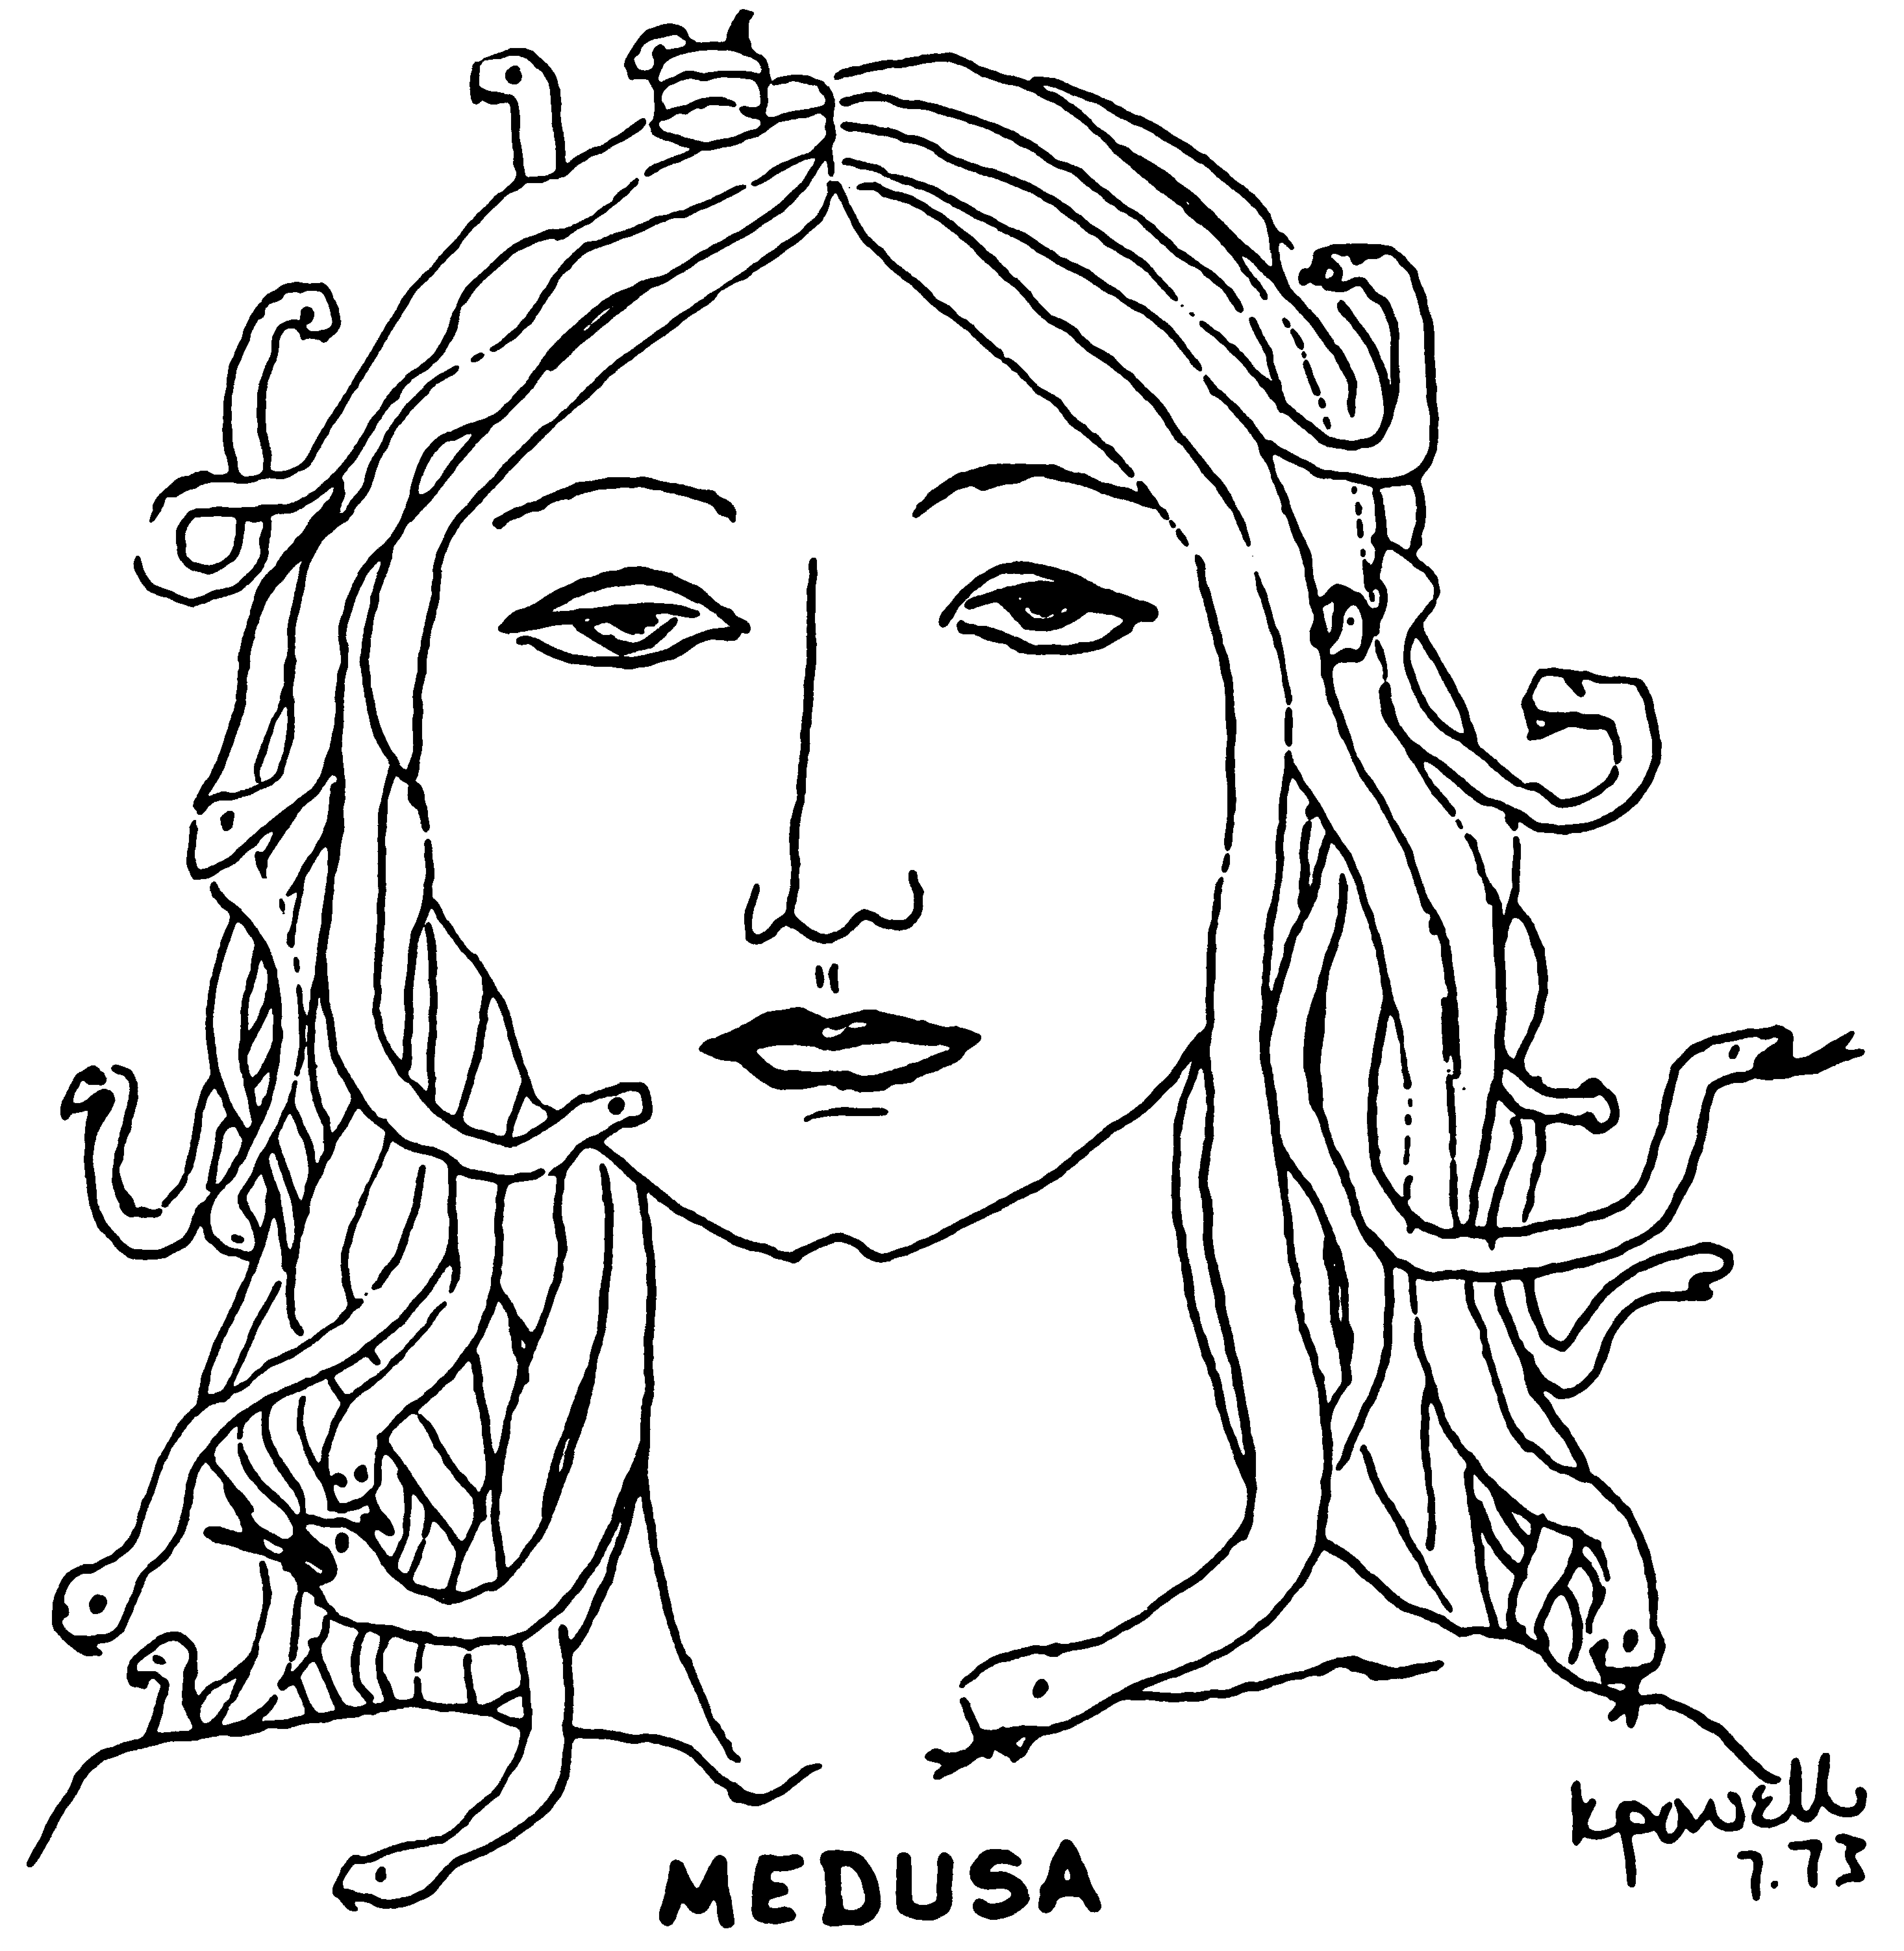
\includegraphics[scale=0.042]{./images/medusa.jpg}
\end{center}

\begin{tabular}[t]{p{3cm}p{12cm}}
\multicolumn{2}{l}{\myunderline{\textbf{Table des Capacités Extraordinaires}}} \\
\textbf{\myunderline{Jet de dé}} & \myunderline{\textbf{Capacité}} \\
01--10 & Clairaudience \\
11--20 & Clairvoyance \\
21--30 & Perception extra-sensorielle (ESP) \\
31--40 & Télépathie \\
41--50 & Télékinésie \\
51--59 & Téléportation \\
60--68 & Vision rayons X \\
69--77 & Génération d'illusions \\
78--82 & Lévitation \\
83--87 & Vol \\
88--92 & Soins (1 point par 6 tours ou 6 points par jour) \\
93--97 & 1--4 fois la force normale pendant 1--10 tours, peut être employé une fois par jour \\
98-99 & Refaire deux jets en ignorant les jets au-dessus de 97 \\
\hspace{0.4cm}00 & Refaire trois jets en ignorant les jets au-dessus de 97 \\
\end{tabular}

\medskip

Tous les Pouvoirs Primaires et Capacités Extraordinaires sont transmis à l'utilisateur de l'épée. Si vous tirez la même capacité deux fois , cela signifie que la capacité est doublée en termes de force, de portée, de précision, etc.

\bigskip

\myunderline{\textbf{Egoïsme}} : seules les épées avec une Intelligence de 7 ou plus ont un score d'Egoïsme. L'Egoïsme est compris dans l'intervalle 1--12, plus le nombre est grand et plus grand est l'Egoïsme de l'épée. L'Egoïsme de l'épée peut lui faire faire les choses suivantes :

\begin{enumerate}
\item Obliger l'utilisateur à se défaire de meilleures armes,
\item Mettre l'utilisateur dans des situations très dangereuses afin d'exalter son rôle dans le combat,
\item Se laisser capturer par un personnage ou une créature de niveau plus élevé qui est plus proche de l'esprit de l'épée,
\item Se laisser capturer par un personnage ou une créature de niveau plus faible dans le but d'exercer un plus grand contrôle sur son utilisateur, et
\item Exiger qu'une partie des trésors conquis lui soit consacré, sous la forme de meilleurs fourreaux, d'incrustations de joyaux, ou de dispositifs magiques pour la garder lorsque personne ne l'utilise.
\end{enumerate}

A chaque moment où une situation se présente durant laquelle une des possibilités listées ci-dessus existe, l'Egoïsme de l'épée intervient. Ce dernier influencera toujours sa relation à l'utilisateur, bien que de vrais rapports puissent voir le jour si l'alignement et les buts du personnage/utilisateur coïncident avec l'\myunderline{origine/objectife} de l'épée. La détermination de chaque facteur est décrite ci-après:

\begin{center}
\begin{minipage}{0.8\linewidth}
\textbf{Influence de l'Egoïsme dans des Situations Clef} : l'arbitre additionne l'Intelligence et l'Egoïsme de l'épée (entre 8 et 24) et ajoute 1 pour chaque Capacité Extraordinaire (entre 1 et 4 si applicable). Le total (dans l'intervalle 8--28) est comparé à la somme de l'Intelligence et de la Force du personnage (6--36) modifié par une variable basée sur l'état physique de l'utilisateur. Si le personnage est frais et relativement exempt de dommages (moins de 10\% de dommages), il faut \myunderline{ajouter} 1--6 points à son total (pour arriver à un intervalle de 7--42). S'il est mentalement ou physiquement fatigué, ou s'il a subi des dommages compris entre 10\% et 50\%, il faut \myunderline{déduire} 1--4 points de son total (pour arriver à un intervalle de 2--35). Si les dommages subis dépassent les 50\%, ou le personnage a été sous le coup d'une tension mentale sévère venant d'une forme de magie, il faut \myunderline{déduire} 2--8 points (pour arriver à un intervalle de 0--34).

\bigskip

{\parindent0.5cm \begin{tabular}{ll}
\textbf{\myunderline{Différence}} & \myunderline{\textbf{Résultat}} \\
6 ou plus & Le plus haut score l'emporte \\
2--5 & 75\% de chances que le plus haut score l'emporte \\
0--1 & 50\% de chances pour chacun \\
\end{tabular}}

\bigskip

\textbf{L'Egoïsme dans les relations au long cours avec l'utilisateur} : cette détermination est assez simple, car elle est basée sur la comparaison du score d'Egoïsme de l'épée (1--12) avec le niveau du guerrier l'utilisant. Consultez la table des \myunderline{Situations Clef} ci-dessus. Si l'une des parties a une différence positive de 6 ou plus, celle-ci l'emportera toujours et plus aucun test (incluant les Situations Clef) ne sera nécessaire. Une différence positive de 2--5 indiquera que celle ayant le plus haut score l'emporte généralement, et les tests ne devront être effectués que dans les Situations Clef. Une différence de 0--1 indique un combat continu entre l'épée et son utilisateur, et durant les situations stressantes, les deux devraient être testés afin de déterminer qui l'emporte.

\end{minipage}
\end{center}

\myunderline{\textbf{Origine/Objectif}} : naturellement, l'origine de chaque épée est la Loi, la Neutralité ou le Chaos, mais certaines de ces armes sont forgés par des forces plus puissantes pour un objectif particulier. Pour déterminer si une épée possède un tel objectif, faire un jet de pourcentage et un jet de 91 ou plus indique que l'épée possède une mission spéciale. Les épées avec des objectifs spéciaux voient automatiquement leur score l'Intelligence et d'Egoïsme poussés au maximum et elles gagnent une capacité additionnelle :

\bigskip

{\parindent1cm \textbf{Loi}: capacité de paralyser les opposants chaotiques,

\textbf{Neutralité} : ajoute +1 à tous les jets de sauvegarde,

\textbf{Chaos} : capacité de désintégrer les opposants loyaux.}

\bigskip

La capacité spéciale ne sera applicable que pour ceux que l'épée a été chargée de détruire, ou ceux qui les servent.

\myunderline{\textbf{Objectifs}}:

\medskip

{\parindent1.5cm\begin{tabular}{p{4.6cm}p{4.6cm}p{4.6cm}}
Tuer les magiciens & Tuer les guerriers & Vaincre la Loi \\
Tuer les clercs & Tuer les monstres & Vaincre le Chaos \\
\end{tabular}}

\bigskip

Ainsi, une épée au service de la Loi ayant pour but de tuer les magiciens (chaotiques) les paralysera ainsi que leurs sbires, mais elle n'utilisera pas ses pouvoirs de paralysie contre un géant errant. Néanmoins, les épées ayant un objectif large utiliseraient leurs pouvoirs pour vaincre tous les opposants de nature Loyale ou Chaotique. Les épées ayant un objectif spécial de Neutralité agiront contre la Loi et le Chaos de la même manière. Les épées ayant un objectif spécial chercheront toujours à l'accomplir, et chaque tentative des utilisateurs de le contrer se soldera immédiatement par un test d'influence.

\bigskip

\myunderline{\textbf{EPEES, BONUS AUX DOMMAGES}} : Les épées reçoivent toutes des bonus pour ce qui est de la probabilité de toucher un opposant, mais certaine sd'entre elles reçoivent aussi un bonus aux dommages quand elles touchent. Ces épées sont celles qui ont un +2 ou +3 contre certaines créatures, mais pas celles qui ont un bonus général de +2 ou +3.



%- - - - - - - - - - - - - - - - - - - - - - - - - - - SUB SUB SECTION
\phantomsection\subsubsection*{DIVERS OBJETS MAGIQUES :}
\addcontentsline{toc}{subsubsection}{DIVERS OBJETS MAGIQUES}

\label{objet-boule-cristal}\textbf{Boules de cristal} : généralement, l'utilisation réussie de ces objets est mise à mal par les grandes distances, le fait de ne pas connaître vraiment le sujet, quand des sorts sont utilisés pour empêcher cette utilisation, quand du plomb s'interpose entre le magicien et le sujet, etc. Seulement trois tentatives par jour peuvent être faites dans les circonstances mentionnées ci-dessus pour ne pas rendre fou le magicien. Une utilisation longue de la boule de cristal demande au magicien de se reposer et de récupérer le jour suivant. Les sorts ne peuvent pas être lancés au travers d'une boule de cristal, mais l'opérateur peut, par exemple, lancer un sort d'infravision sur lui-même, puis regarder dans l'objet et voir dans les ténèbres.

\bigskip

\phantomsection\label{objet-medaillon-esp}\textbf{Médaillons de perception extrasensorielle} : ces objets sont utilisables par toutes les classes de personnages, même les Nains. Lancer 1d6 à leur utilisation ; ils dysfonctionnent si l'obtient 6.

\bigskip

\phantomsection\label{objet-amulette-captation}\textbf{Amulette de captation} : fonctionne avec une boule de cristal ou l'utilisation du sort Perception extrasensorielle\footnote{Voir page \pageref{sort-esp} (NdT).}. Cet objet donne la localisation, la vision, ou les pensées récupérées par la boule de cristal ou l'utilisation du sort. Il fonctionne toujours.

\bigskip

\phantomsection\label{objet-heaume-telepathie}\textbf{Heaume de télépathie} : permet au porteur de lire les pensées de toute créature dans un rayon de 3m. Si son Intelligence est plus grande que la créature humaine ou humanoïde dans la portée du heaume, le porteur peut tenter de contrôler leur esprit avec des suggestions implantées de manière télépathique. De telles suggestions auront un effet de +2 dans leur probabilité d'être suivies (voir Vol. III pour les actions aléatoires des monstres\footnote{Voir section \og Actions aléatoires par monstre \fg{} de ce document.}). Pour les personnages du jeu, faites un jet de pourcentage en ajoutant 10\% au porteur du heaume, et si le personnage échoue à battre son score,%Quel score?
il suivra la suggestion. (L'arbitre doit utiliser son jugement dans ce cas, car une suggestion de se suicider ne devrait pas avoir de chances d'être suivie par un événement.) Traiter comme un heaume non protégeant si le casque est porté en mêlée.

}% parindent




%+=+=+=+=+=+=+=+=+=+=+=+=+=+=+=+=+=+=+=+=+=+=+=+=+=+=+=+=+=+=+=+=+=+=+=+= PART
%+=+=+=+=+=+=+=+=+=+=+=+=+=+=+=+=+=+=+=+=+=+=+=+=+=+=+=+=+=+=+=+=+=+=+=+= PART
%+=+=+=+=+=+=+=+=+=+=+=+=+=+=+=+=+=+=+=+=+=+=+=+=+=+=+=+=+=+=+=+=+=+=+=+= PART
%+=+=+=+=+=+=+=+=+=+=+=+=+=+=+=+=+=+=+=+=+=+=+=+=+=+=+=+=+=+=+=+=+=+=+=+= PART
%+=+=+=+=+=+=+=+=+=+=+=+=+=+=+=+=+=+=+=+=+=+=+=+=+=+=+=+=+=+=+=+=+=+=+=+= PART
\newpage
\phantomsection\addcontentsline{toc}{section}{D\&D VOLUME III -- AVENTURES DANS LE MONDE SOUTERRAIN \& DANS LES REGIONS SAUVAGES}\begin{center}
{\Huge \ODDtitlefont{DONJONS \& DRAGONS}}{\normalsize \textsuperscript{\sffamily\textregistered}}

\vspace{1.8cm}

{\Large \textbf{Volume III}}

\vspace{1.3cm}

{\Huge \ODDtitlebisfont{AVENTURES}}

\vspace{0.3cm}

{\Huge \ODDtitlebisfont{DANS LE MONDE}}

\vspace{0.3cm}

{\Huge \ODDtitlebisfont{SOUTERRAIN}}

\vspace{0.3cm}

{\Huge \ODDtitlebisfont{ \& DANS LES}}

\vspace{0.3cm}

{\Huge \ODDtitlebisfont{REGIONS}}

\vspace{0.3cm}

{\Huge \ODDtitlebisfont{SAUVAGES}}

\vspace{3cm}

{\large PAR

\vspace{0.1cm}

GARY GYGAX \& DAVE ARNESON}
\end{center}

\newpage
%======================Blank page
\phantom{-}
\newpage

%==========================================================================SECTION
\newpage
\phantomsection\section*{Aventures dans le monde souterrain \& dans les régions sauvages}
\addcontentsline{toc}{section}{Aventures dans le monde souterrain \& dans les régions sauvages}

\begin{center}
\textbf{[SELECTION]}
\end{center}

%----------------------------------------------------- SUB SECTION
\phantomsection\subsection*{LES MONSTRES DU MONDE SOUTERRAIN}
\addcontentsline{toc}{subsection}{LES MONSTRES DU MONDE SOUTERRAIN}

\pdfbookmark[3]{Actions aléatoires par monstre}{pdf-action-monstres}\phantomsection\label{dd3-actions-monstres}\textbf{Actions aléatoires par monstre} : dans les autres situations qu'en poursuite, les plus intelligents des monstres agiront de manière aléatoire, en accord avec les résultats obtenus en faisant un jet de deux dés (à six faces) :

\bigskip

{\parindent6cm \begin{tabular}{cl}
2--5 & réaction négative \\
6--8 & réaction incertaine \\
9--12 & réaction positive \\
\end{tabular}}

\medskip

Le score aux dés doit être modifié par des additions ou des soustractions pour des choses telles que des pots-de-vin offerts, la peur, l'alignement des parties concernées, etc.



%+=+=+=+=+=+=+=+=+=+=+=+=+=+=+=+=+=+=+=+=+=+=+=+=+=+=+=+=+=+=+=+=+=+=+=+= PART
%+=+=+=+=+=+=+=+=+=+=+=+=+=+=+=+=+=+=+=+=+=+=+=+=+=+=+=+=+=+=+=+=+=+=+=+= PART
%+=+=+=+=+=+=+=+=+=+=+=+=+=+=+=+=+=+=+=+=+=+=+=+=+=+=+=+=+=+=+=+=+=+=+=+= PART
%+=+=+=+=+=+=+=+=+=+=+=+=+=+=+=+=+=+=+=+=+=+=+=+=+=+=+=+=+=+=+=+=+=+=+=+= PART
%+=+=+=+=+=+=+=+=+=+=+=+=+=+=+=+=+=+=+=+=+=+=+=+=+=+=+=+=+=+=+=+=+=+=+=+= PART
\newpage
\phantomsection\addcontentsline{toc}{section}{SUPPLEMENT I -- GREYHAWK}\begin{center}
{\Huge \ODDtitlefont{DONJONS \& DRAGONS}}{\normalsize \textsuperscript{\sffamily\textregistered}}

\vspace{1.8cm}

{\Large \textbf{Supplément I}}

\vspace{1.3cm}

{\Huge \ODDtitlebisfont{GREYHAWK}}

\vspace{5cm}

{\large PAR

\vspace{0.1cm}

GARY GYGAX \& ROB KUNTZ}
\end{center}

\newpage
%======================Blank page
\phantom{-}
\newpage


%==========================================================================SECTION
\phantomsection\section*{Hommes \& Magie}
\addcontentsline{toc}{section}{Hommes \& Magie}

\begin{center}
\textbf{[SELECTION]}
\end{center}

%----------------------------------------------------- SUB SECTION
\phantomsection\subsection*{SYSTEME DE COMBAT ALTERNATIF}
\addcontentsline{toc}{subsection}{SYSTEME DE COMBAT ALTERNATIF}
\label{combat-alternatif}

Pour ceux qui voudraient inclure les types d'armes dans la détermination des probabilités de toucher, le tableau suivant, extrait de la section \og combat en mêlée \fg{} de CHAINMAIL est offert. Si ce système est utilisé, il est suggéré d'employer le tableau des dommages par type d'arme et type de monstre.

Traiter les Voleurs et Clerc en termes d'avancement en paliers -- quatre niveaux/groupe (1--4, 5--8, 9--12, etc.). En ce qui concerne les jets de sauvegarde, traiter les Voleurs comme des magiciens.

\bigskip

%\begin{tabular}{lcccccccc}
\begin{tabular}{l>{\centering\arraybackslash}p{1.2cm}>{\centering\arraybackslash}p{1.2cm}>{\centering\arraybackslash}p{1.2cm}>{\centering\arraybackslash}p{1.2cm}>{\centering\arraybackslash}p{1.2cm}>{\centering\arraybackslash}p{1.2cm}>{\centering\arraybackslash}p{1.2cm}>{\centering\arraybackslash}p{1.2cm}}
\multicolumn{1}{c}{\textit{Type d'arme}} & \multicolumn{8}{c}{\textit{Classe d'armure du défenseur}} \\
\multicolumn{1}{c}{\textit{de l'attaquant}}  &  \textit{2} &  \textit{3} &  \textit{4} &  \textit{5} &  \textit{6} &  \textit{7} &  \textit{8} &  \textit{9} \\
&&&&&&&&\\
Dague*            & -3 & -3 & -1 & -1 &  0 &  0 & +1 & +2 \\
Hache à main      & -3 & -2 & -1 & -1 &  0 &  0 & +1 & +1 \\
Masse             &  0 & +1 &  0 &  0 &  0 &  0 &  0 &  0 \\
Marteau           &  0 & +1 &  0 & +1 &  0 &  0 &  0 &  0 \\
Epée*             & -2 & -1 &  0 &  0 &  0 &  0 &  0 & +1 \\
Piolet            & +2 & +3 & +2 & +3 &  0 &  0 &  0 &  0 \\
Hache de bataille & -1 &  0 & +1 & +1 &  0 &  0 &  0 &  0 \\
Masse à pointes   &  0 &  0 & +1 & +2 & +1 & +1 & +2 & +2 \\
Fléau d'armes     & +2 & +2 & +1 & +2 & +1 & +1 & +1 & +1 \\
Lance*            & -2 & -1 & -1 & -1 &  0 &  0 &  0 &  0 \\
Arme d'hast*      & -1 &  0 &  0 & +1 & +1 & +2 & +2 & +2 \\
Hallebarde*       &  0 & +1 & +1 & +2 & +1 &  0 &  0 &  0 \\
Epée à deux mains & +1 & +2 & +3 & +3 & +2 & +2 & +2 & +2 \\
Lance de tournoi  &  0 &  0 & +1 & +2 & +3 & +3 & +3 & +3 \\
Pique             & -1 &  0 &  0 &  0 &  0 &  0 &  0 &  0 \\
\multicolumn{9}{l}{..................} \\
Arc court (15)       & \footnotesize-3-5-7 & \footnotesize-2-3-5 & \footnotesize0-1-2
& \footnotesize0 0-1 & \footnotesize+1 0 0 & \footnotesize+2+1 0
& \footnotesize+2+1 0 & \footnotesize+2+1 0 \\
Arc monté (18)       & \footnotesize-3-4-7 & \footnotesize-2-3-5 & \footnotesize0-1-2 & \footnotesize0 0-1 & \footnotesize+1 0 0 & \footnotesize+2+1 0 & \footnotesize+2+1 0 & \footnotesize+3+2+1 \\
Petite arbalète (18) & \footnotesize-3-5-7 & \footnotesize-2-3-5 & \footnotesize0-1-4 & \footnotesize0 0-1 & \footnotesize+2+1 0 & \footnotesize+3+1 0 & \footnotesize+3+1 0 & \footnotesize+3+2+1 \\
Arc long (21)        & \footnotesize-2-3-5 & \footnotesize 0-2-4 & \footnotesize0 0-1 &\footnotesize+2+1 0 & \footnotesize+3+2+1 & \footnotesize+3+2+1 & \footnotesize+3+2+1 & \footnotesize+3+2+1 \\
Arc composite (24)   & \footnotesize-3-4-5 & \footnotesize 0-3-4 & \footnotesize0-1-2 &\footnotesize+2 0-1 & \footnotesize+3+1 0 & \footnotesize+3+2+1 & \footnotesize+3+2+1 & \footnotesize+3+2+1 \\
Arbalète lourde (24) & \footnotesize-1-2-3 & \footnotesize 0-1-3 &\footnotesize+1 0-1 &\footnotesize+2 0 0 & \footnotesize+3+1 0 & \footnotesize+4+2+1 & \footnotesize+4+2+1 & \footnotesize+4+3+2 \\
Arquebuse (18)       &  \footnotesize0-1-3 & \footnotesize+1 0-1 &\footnotesize+2 0 0 &\footnotesize+2+1 0 & \footnotesize+3+2 0 & \footnotesize+3+2 0 & \footnotesize+3+2 0 & \footnotesize+3+2 0 \\
\end{tabular}

\bigskip

{\parindent1cm * Si l'opposant a mis pied à terre et est prêt, utilisez le tableau ci-dessous :}

\medskip

{\parindent2cm\begin{tabular}{p{3cm}crcccc}
\textit{Type d'arme}&&Classe d'armure --- &  2 &  3 &  4 &  5 \\\cline{4-7}
Indiqués par &&                           & +3 & +2 & +2 & +1 \\
astérisques &&&&&& \\
\end{tabular}}

\bigskip

{\parindent1cm (15)}

{\parindent2cm \parbox{14.5cm}{Les nombres entre parenthèses sont les portées maximales, et les nombres montrés sont pour les portées courte (premier tiers de la portée), moyenne (tiers suivant de la portée) et longue (dernier tiers de la portée).}}

\begin{center}
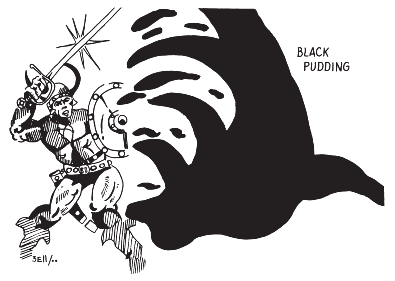
\includegraphics[width=0.8\linewidth]{./images/black-pudding.png}
\end{center}

%- - - - - - - - - - - - - - - - - - - - - - - - - - - SUB SUB SECTION
\phantomsection\subsubsection*{Dommages causés par type d'armes :}
\addcontentsline{toc}{subsubsection}{Dommages causés par type d'armes}

Si le système de dommage variables par type d'armes est utilisé, les divers monstres devront aussi être sujets à recevoir des points de dommages additionnels ou des dés de dommages. (Voir \textbf{Attaques et dommages par type de monstre}).

\bigskip

\begin{tabular}{lccc}
\textit{Type d'armes} & \textit{contre-} & \textit{-Opposants taille humaine-} & \textit{-Opposants plus grands-} \\
Dague                          && 1--4 points  & 1--3 points \\
Hache à main                   && 1--6 points  & 1--4 points \\
Masse, piolet*, marteau de nain && 1--6 points  & 1--4 points \\
Epée                           && 1--8 points  & 1--12 points \\
Hache de bataille*             && 1--8 points  & 1--8 points \\
Masse à pointes**              && 1--8 points  & 1--6 points \\
Fléau d'armes ***              && 1--8 points  & 1--8 points \\
Lance, lancée/enfoncée         && 1--6 points  & 1--8 points \\
Lance, enfoncée contre charge  && 1--8 points  & 2--12 points \\
Lance, posée contre charge     && 1--10 points & 2--16 points \\
Armes d'hast****               && 1--8 points  & 1--12 points \\
Hallebarde***                  && 1--10 points & 2--12 points \\
Epée à deux mains***           && 1--10 points & 3--18 points \\
Lance de tournoi               && 1--8 points  & 2--24 points \\
Pique****                      && 1--8 points  & 1--12 points \\
Flèche ou carreau              && 1--6 points  & 1--6 points \\
Pierre de fronde               && 1--4 points  & 1--6 points \\
\end{tabular}

\begin{tabular}{rp{15cm}}
\multicolumn{1}{r}{*} & l'arme requiert au moins 1.2m d'espace de chaque côté du porteur \\
\multicolumn{1}{r}{**} & l'arme requiert au moins 1.5m d'espace de chaque côté du porteur \\
\end{tabular}

\begin{tabular}{rp{15cm}}
\multicolumn{1}{r}{***} & l'arme requiert au moins 1.8m d'espace de chaque côté du porteur \\
\multicolumn{1}{r}{****} & la règle générale est que ces armes ne sont pas utilisables dans les donjons en raison de leur longueur \\
\end{tabular}

%- - - - - - - - - - - - - - - - - - - - - - - - - - - SUB SUB SECTION
\phantomsection\subsubsection*{Attaques et dommages par type de monstre}
\addcontentsline{toc}{subsubsection}{Attaques et dommages par type de monstre}
\label{greyhawk-dommages-monstres}

Ce système doit être utilisé avec les dommages variables par arme et, en aucun cas, il n'est recommandé de l'utiliser sans la mécanique susmentionnée.

\bigskip

\begin{tabular}{p{4cm}>{\raggedright\arraybackslash}p{5cm}>{\raggedright\arraybackslash}p{6.5cm}}
\textit{Type de monstre} && \textit{Points de dommages} \\
\hspace{0.5cm}\textit{attaquant} & \textit{Nombre d'attaques} & \hspace{0.5cm}\textit{par attaque} \\
Homme & 1 ou 2 & Dépend du type d'arme \\
Gobelin/Kobold & 1 & 1--4 ou par type d'arme \\
Orc & 1 & 1--6 ou par type d'arme \\
Hobgobelin/Gnoll & 1 & 1--8 ou par type d'arme \\
Ogre  & 1 & 1--10 \\
Troll & 2 griffes/1 morsure & 1--4/griffe, 1--8/morsure \\
Géant & 1 & COLLINE --- 2--16 \\
&& PIERRE --- 3--18 \\
&& GIVRE --- 4--24 \\
&& FEU --- 5--30 \\
&& NUAGE --- 6--36 \\
Squelette & 1 & 1--6 \\
Zombie & 1 & 1--8 \\
Goule & 2 griffes/1 morsure & 1--3/griffe, 1--4/morsure \\
Wight & 1 & Drain d'énergie seulement \\
Wraith & 1 & 1--6 et drain d'énergie \\
Momie & 1 & 1--12 \\
Spectre & 1 & 1--8 et drain d'énergie \\
Vampire & 1 & 1--10 et drain d'énergie \\
Cocatrix & 1 & 1--6 et changement en pierre \\
Basilic & 1 & 1--10 et changement en pierre \\
Méduse & 1 ou 2 & par type d'arme et changement en pierre \\
Gorgone* & 1 coup & 2--12/coup \\
Manticore & 2 griffes/1 morsure/24 pics & 1--3/griffe, 1--8/morsure, 1--6/pic \\
Hydre & 1 par tête & 1--6, 1--8, 1--10 selon la taille \\
Chimère & 2 griffes/3 têtes & 1--3/griffe ;\\
&& TETE DE CHEVRE --- 1--4/corne \\
&& TETE DE LION --- 1--8/morsure \\
&& TETE DE DRAGON --- 3-12/morsure** \\
Wyverne & 1 morsure/1 dard & 2-16/morsure, 1-6/dard*** \\
\end{tabular}


\begin{tabular}{p{4cm}>{\raggedright\arraybackslash}p{5cm}>{\raggedright\arraybackslash}p{6.5cm}}
\textit{Type de monstre} && \textit{Points de dommages} \\
\hspace{0.5cm}\textit{attaquant} & \textit{Nombre d'attaques} & \hspace{0.5cm}\textit{par attaque} \\
Dragon* & 2 griffes/1 morsure & 1--4/griffe ; \\
&& BLANC --- 2--16/morsure \\
&& NOIR --- 3--18/morsure \\
&& VERT --- 2--20/morsure \\
&& BLEU --- 2--24/morsure \\
&& ROUGE --- 3--30/morsure \\
&& DORE --- 3--36/morsure \\
Gargouille & 2 griffes/1 morsure/1 corne & 1--3/griffe, 1--6/morsure, 1--4/corne \\
Lycanthrope & LOUP --- 1 morsure & 2--8/morsure \\
& SANGLIER --- 1 morsure & 2--12/morsure \\
& TIGRE --- 2 griffes/1 morsure & 1--4/griffe, 1--10/morsure \\
& OURS --- 2 griffes/1 morsure & 1--3/griffe****, 2--8/morsure \\
Vert pourpre & 1 morsure/1 piqûre & 2-24/morsure, 1-8/piqûre*** \\
Monstre marin & 1/tête ou /tentacule ou par griffe & entre 3--24 et 5--50/tête, ou 2--12 et 4--24/tentacule ou 2--8 et 4--32/griffe \\
Minotaure & 1 coup/1 morsure/1 arme & 2--8/coup, 1--3/morsure, par type d'arme \\
Centaure & 2 sabots/1 arme & 1--6/sabot, par type d'arme \\
Licorne & 2 sabots/1 corne & 1--8/sabot, 1-16/corne \\
Nixe & 1 & 1--4 ou par type d'arme \\
Dryade & 1 & 1--4 ou par type d'arme \\
Gnome & 1 & 1--6 ou par type d'arme \\
Nain & 1 & 1--8 ou par type d'arme \\
Elfe & 1 & 1--10 ou par type d'arme \\
Ent & 2 & 2--16, 3--18, ou 4--24/attaque selon taille \\
Pégase & 2 sabots & 1--8/sabot \\
Hippogriffe & 2 griffes/1 morsure & 1--6/griffe, 1--10/morsure \\
Rokh & 2 griffes/1 morsure & 1--8, 2--12 ou 4--16/griffe, 2--12, 3--18 ou 4--24/morsure selon taille \\
Griffon & 2 griffes/1 morsure & 1--4/griffe, 2--16/morsure \\
Harceleur invisible & 1 & 4--16 \\
Elémentaire***** & 1 & AIR --- 2--16 \\
&& TERRE --- 4--32 \\
&& FEU --- 3--24 \\
&& EAU --- 3--30 \\
Djinn & 1 & 2--16 \\
Efrit & 1 & 3--24 \\
Gelée ocre & 1 & 2--12 \\
Black Pudding & 1 & 3--24 \\
Slime vert & 1 & spécial \\
Vase grise & 1 & 2--16 \\
\end{tabular}

\begin{tabular}{p{4cm}>{\raggedright\arraybackslash}p{5cm}>{\raggedright\arraybackslash}p{6.5cm}}
\textit{Type de monstre} && \textit{Points de dommages} \\
\hspace{0.5cm}\textit{attaquant} & \textit{Nombre d'attaques} & \hspace{0.5cm}\textit{par attaque} \\
Moisissure jaune & 1 & spécial \\
Petit cheval & 2 sabots & 1--4/sabot \\
Cheval moyen & 2 sabots/1 morsure & 1--6/sabot, 1-3/morsure \\
Grand cheval & 2 sabots/1 morsure & 1--8/sabot, 1-3/morsure \\
Rat géant (de Sumatra) & 1 morsure & 1-3/morsure \\
Loup & 1 morsure & 1-6/morsure \\
Canis Dirus & 1 morsure & 1-8/morsure \\
Lion & 2 griffes/1 morsure & 1--3/griffe, 1--10/morsure \\
Tigre à dents de sabre & 2 griffes/1 morsure & 1--4/griffe, 2--12/morsure \\
Belette géante & 1 morsure & 2--8/morsure plus drain de sang \\
Mammouth & 2 défenses/1 tronc/2 pieds & 3--18/défense, 2--16/tronc,
2--12/pied \\
Araignée géante & 1 morsure & 1--3*** plus toiles \\
Lézard géant & 1 morsure & 1--8/morsure \\
Crapaud géant & 1 morsure & 1--10/morsure \\
Serpent géant & 1 morsure, une constriction & 1--6/morsure***, 2--8/tour de constriction \\
Crabe géant & 2 pinces & 2--12/pince \\
Scarabée géant & 1 morsure & 3--30/morsure \\
Scorpion géant & 2 pinces/1 dard & 1--10/pince, 1--4***/dard \\
Crocodile & 1 morsure & 3--12/morsure \\
Tyrannosaurus rex & 1 morsure & 5--40/morsure \\
Triton & 1 & 3--18 plus spécial \\
Bugbear & 1 & 2--8 \\
Ogre mage & 1 & 1--12 \\
Géant, ORAGE & 1 & 7--42 \\
Titan & 1 & 7--42 \\
Ombre & 1 & 1--4 plus spécial \\
Feu follet & spécial & spécial \\
Liche & 1 & 1--10 plus spécial \\
Harpie & 2 griffes/1 arme & 1--3/griffe, 1--6/arme \\
Homme-lézard & 2 griffes/1 morsure & 1--3/griffe, 1--8/morsure \\
Doppleganger & 1 & 1--12 plus spécial \\
Dragon & 2 griffes/1 morsure & 1--4/griffe \\
&& AIRAIN --- 4--16/morsure \\
&& CUIVRE --- 5--20/morsure \\
&& BRONZE --- 3--24/morsure \\
&& ARGENT --- 3-30/morsure \\
Lycanthrope : Rat-garou ou homme-rat & 1 morsure/1 arme & 1--3/morsure, par type d'arme \\
Lammasu & 2 griffes & 1--6/griffe plus spécial \\
\end{tabular}

\begin{tabular}{p{4cm}>{\raggedright\arraybackslash}p{5cm}>{\raggedright\arraybackslash}p{6.5cm}}
\textit{Type de monstre} && \textit{Points de dommages} \\
\hspace{0.5cm}\textit{attaquant} & \textit{Nombre d'attaques} & \hspace{0.5cm}\textit{par attaque} \\
Salamandre***** & 1 touché/1 constriction/1 arme & spécial, 2--8/tour de constriction, par type d'arme \\
Beholder & 1 morsure & 2--5 plus spécial \\
Mastodonte des ombres & 2 griffes/1 morsure & 1--12/griffe, 2--8/morsure \\
Bête éclipsante & 2 tentacules & 2--8/tentacule \\
Chien esquiveur & 1 morsure & 1--6/morsure \\
Chien de chasse infernal* & 1 morsure & 1--6/morsure \\
Araignée de phase & 1 morsure & 1--6/morsure*** \\
Oxydeur & 1 toucher & spécial \\
Stirge & 1 morsure & 1--3 plus draine le sang \\
Tique géante & 1 morsure & 1--4 plus draine le sang \\
Ours-Hiboux & 2 griffes/1 morsure & 1--6/griffe****, 2--12/morsure \\
Charognard rampant & 8 tentacules & spécial \\
Cube gélatineux & 1 & 2--8 spécial \\
Limace géante & 1 morsure & 1--12 plus spécial \\
Homoncule & 1 morsure & 1--3 plus spécial \\
Golem & 1 & CHAIR --- 2--16 \\
&& PIERRE --- 3--24 \\
&& FER --- 4--32 \\
\end{tabular}
\begin{tabular}{rp{14.5cm}}
\multicolumn{1}{r}{*} & possèdent aussi leur souffle comme arme \\
\multicolumn{1}{r}{**} & à moins que le souffle soit utilisé \\
\multicolumn{1}{r}{***} & quelque soit le résultat, jet de sauvegarde contre le poison \\
\multicolumn{1}{r}{****} & une étreinte avec un score de 18 ou plus cause 2--16 points de dommages supplémentaires \\
\multicolumn{1}{r}{*****} & voir les différentes sections concernant tous les types d'élémentaires car des ajustements pourraient être requis en raison des circonstances
\end{tabular}

%----------------------------------------------------- SUB SECTION
\phantomsection\subsection*{EXPLICATION DES SORTS :}
\addcontentsline{toc}{subsection}{EXPLICATION DES SORTS}

%- - - - - - - - - - - - - - - - - - - - - - - - - - - SUB SUB SECTION
\phantomsection\subsubsection*{\textit{Magiciens :}}
\addcontentsline{toc}{subsubsection}{Magiciens}

\textit{Troisième niveau :}

\bigskip

\label{sort-suggestion}\textbf{Suggestion} : un sort qui fonctionne que le principe de l'hypnose. Si une créature sur laquelle le sort est lancé rate son jet de sauvegarde contre la magie, elle sera la victime de la suggestion, immédiatement ou de manière différée au bon vouloir du magicien. Le fait que la créature s'autodétruise est improbable à 99\%, mais des suggestions formulées avec attention peuvent, selon l'estimation de l'arbitre, altérer cette probabilité. Les suggestions doivent être simples et relativement courtes, soit une phrase ou deux. Durée : une semaine de temps de jeu.

\bigskip

\textit{Neuvième niveau :}

\bigskip

\phantomsection\label{sort-astral}\textbf{Sort astral} : un sort qui permet à l'utilisateur d'envoyer sa forme astrale, indétectable pour tous sauf pour ceux du plan astral, depuis son corps vers d'autres endroits. Noter qu'un sort ``Mot de pouvoir aveuglant'' ne pourrait pas empêcher ce sort et ne pourrait pas aveugler la forme astrale. Le magicien peut utiliser des sorts quand il est dans sa forme astrale, mais il y a 5\% de risques par niveau de sort que le sort échoue. Si le sort échoue, il y a un risque de 2\% par niveau de sort que le magicien soit forcé de retourner dans son corps. Exemple : un magicien du dix-huitième niveau dans sa forme astrale tente de jeter un sort du sixième niveau. Il y  30\% de chances que le sort échoue, et s'il échoue, il y a 12\% de chances qu'il soit obligé de réintégrer son corps. Si, pendant que le magicien a quitté son corps et se trouve dans le plan astral, son corps est bougé en dehors de la porté du sort ou détruit, la forme astrale du magicien est immédiatement envoyée pour bafouiller et hurler au plus bas niveau de l'enfer. Durée : dans les souterrains -- 12 tours ; à l'extérieur -- 8 heures de jeu. Portée : dans les souterrains -- 7m ; à l'extérieur -- 160km/niveau à partir du 18\textsuperscript{ème}. Mouvement du corps astral : dans les souterrains -- 4m/tour ; à l'extérieur 160km par heure de jeu depuis le 18\textsuperscript{ème} niveau.


%==========================================================================SECTION
\newpage
\phantomsection\section*{Monstres \& Trésors}
\addcontentsline{toc}{subsection}{Monstres \& Trésors}

\begin{center}
\textbf{[SELECTION]}
\end{center}

%----------------------------------------------------- SUB SECTION
\phantomsection\subsection*{DESCRIPTION DES MONSTRES}
\addcontentsline{toc}{subsection}{DESCRIPTION DES MONSTRES}

\label{monstre-geant-des-tempetes}GEANT DES TEMPETES : ces créatures ne peuvent être trouvés que dans les endroits reculés. Typiquement, leur demeure sera un chateau construit sous les eaux ou sur une montagne ou sur un nuage. Elles sont intelligentes, mesurent à peu près 8m de hauteur et font 3 + 3 dés de dommages (à moins que le système de dommages alternatif ne soit utilisé\footnote{Voir page \pageref{greyhawk-dommages-monstres}.}). Ces géants sont capables d'utiliser le sort Contrôle du climat pour créer une tempête -- leur météo favorite -- quand ils sont en colère ou dans une bataille.

%----------------------------------------------------- SUB SECTION
\phantomsection\subsection*{EXPLICATION DES OBJETS MAGIQUES}
\addcontentsline{toc}{subsection}{EXPLICATION DES OBJETS MAGIQUES}

%- - - - - - - - - - - - - - - - - - - - - - - - - - - SUB SUB SECTION
\phantomsection\subsubsection*{POTIONS :}
\addcontentsline{toc}{subsubsection}{POTIONS}

\label{objet-huile-etheree}\textit{Huile éthérée} : quand l'utilisateur est oint de cette substance, il est capable de traverser des substance solides comme il le souhaite, comme s'il revêtait l'Armure Ethérée. Noter que quand l'utilisateur est ainsi oint, il n'est pas capable de manipuler des objets normaux car ses mains leur passent au travers.


%+=+=+=+=+=+=+=+=+=+=+=+=+=+=+=+=+=+=+=+=+=+=+=+=+=+=+=+=+=+=+=+=+=+=+=+= PART
%+=+=+=+=+=+=+=+=+=+=+=+=+=+=+=+=+=+=+=+=+=+=+=+=+=+=+=+=+=+=+=+=+=+=+=+= PART
%+=+=+=+=+=+=+=+=+=+=+=+=+=+=+=+=+=+=+=+=+=+=+=+=+=+=+=+=+=+=+=+=+=+=+=+= PART
%+=+=+=+=+=+=+=+=+=+=+=+=+=+=+=+=+=+=+=+=+=+=+=+=+=+=+=+=+=+=+=+=+=+=+=+= PART
%+=+=+=+=+=+=+=+=+=+=+=+=+=+=+=+=+=+=+=+=+=+=+=+=+=+=+=+=+=+=+=+=+=+=+=+= PART
%+=+=+=+=+=+=+=+=+=+=+=+=+=+=+=+=+=+=+=+=+=+=+=+=+=+=+=+=+=+=+=+=+=+=+=+= PART
%+=+=+=+=+=+=+=+=+=+=+=+=+=+=+=+=+=+=+=+=+=+=+=+=+=+=+=+=+=+=+=+=+=+=+=+= PART
%+=+=+=+=+=+=+=+=+=+=+=+=+=+=+=+=+=+=+=+=+=+=+=+=+=+=+=+=+=+=+=+=+=+=+=+= PART
\newpage
\phantomsection\addcontentsline{toc}{section}{SUPPLEMENT III bis -- ELDRITCH WIZARDRY}\begin{center}
{\Huge \ODDtitlefont{DONJONS \& DRAGONS}}{\normalsize \textsuperscript{\sffamily\textregistered}}

\vspace{1.8cm}

{\Large \textbf{Supplément III bis}}

\vspace{1.3cm}

{\Huge \ODDtitlebisfont{ELDRITCH}}

\vspace{0.3cm}

{\Huge \ODDtitlebisfont{WIZARDRY}}

\vspace{2.0cm}

{\Large \textbf{MAGIE ANCIENNE ET PUISSANTE}}

\vspace{0.5cm}

{\Large \textbf{POUVOIRS PSIONIQUES}}

\vspace{1cm}

{\large PAR

\vspace{0.1cm}

GARY GYGAX \& BRIAN BLUME \& ROUBOUDOU}
\end{center}

\newpage
%==========================================================================SECTION
\phantomsection\section*{Hommes \& Magie}
\addcontentsline{toc}{section}{Hommes \& Magie}

\begin{center}
\textbf{[POUVOIRS PSIONIQUES]}
\end{center}

%----------------------------------------------------- SUB SECTION
\phantomsection\subsection*{Introduction}
\addcontentsline{toc}{subsection}{Introduction}

Les pouvoirs psioniques sont divisés en deux catégories :

\bigskip

\begin{itemize}
\item Les aptitudes psioniques, des compétences psioniques ressemblant parfois à des sorts ;
\item Les modes d'attaques et de défenses psioniques, servant dans le combat psionique.
\end{itemize}

\bigskip

Chaque pouvoir, lorsqu'il est utilisé, aura généralement un coût en points de \textbf{force psionique (FP)}.

L'acquisition des modes d'attaques et de défense psioniques est liée à l'acquisition des aptitudes psioniques. Dans la partie qui suit, nous détaillons d'abord l'acquisition des aptitudes puis celle des modes d'attaques et de défense psioniques avant de passer au combat psionique à proprement parler.

%----------------------------------------------------- SUB SECTION
\phantomsection\subsection*{Conditions d'accès aux pouvoirs psioniques}
\addcontentsline{toc}{subsection}{Conditions d'accès aux pouvoirs psioniques}

Les conditions suivantes doivent être remplies :

\bigskip

\begin{itemize}
\item Etre humain,
\item Pas de restriction de classe\footnote{L'édition originale indique que les moines ou les druides ne peuvent pas avoir de pouvoirs mentaux, sans que cette restriction ne soit vraiment expliquée. Plus loin, dans la description des aptitudes psychiques, les aptitudes sont données pour les clercs, les moines et les druides. Nous avons donc choisi, dans cette synthèse, de ne pas retenir la restriction de classes.}
\item Avoir un score non modifié de 15 en Intelligence, Sagesse ou Charisme,
\item Faire plus de 90 (91--100) sur un jet de pourcentage (une chance sur 10).
\end{itemize}

\bigskip

Les personnages ayant des pouvoirs psioniques deviennent sensibles aux monstres ayant des capacités psioniques.

%----------------------------------------------------- SUB SECTION
\phantomsection\subsection*{Potentiel psychique}
\addcontentsline{toc}{subsection}{Potentiel psychique}

Lorsque le personnage a accès pour la première fois aux pouvoirs psioniques, le joueur fait un jet de 1d100 pour déterminer le potentiel psychique (voir table ci-dessous).
\bigskip

{\parindent3cm\begin{tabular}{cl}
\textbf{Potentiel psychique} & \textbf{Chance de gagner une aptitude} \\
01--10 & niveau x 4\% \\
11--25 & niveau x 5\% \\
26--50 & niveau x 6\% \\
51--75 & niveau x 10\% \\
76--90 & niveau x 11\% \\
91--99 & niveau x 12\% \\
\hspace{0.4cm}00 & niveau x 13\% \\
\end{tabular}}

%----------------------------------------------------- SUB SECTION
\phantomsection\subsection*{Aptitudes psioniques}
\addcontentsline{toc}{subsection}{Aptitudes psioniques}

%- - - - - - - - - - - - - - - - - - - - - - - - - - - SUB SUB SECTION
\phantomsection\subsubsection*{\textit{Gain d'aptitudes}}
\addcontentsline{toc}{subsubsection}{Gain d'aptitudes}
\label{aptitudes-gain}

Le joueur peut tenter de gagner une ou deux aptitudes psioniques dans deux conditions :

\bigskip

\begin{itemize}
\item Il vient de calculer son potentiel psychique et a accès pour la première fois aux pouvoirs psioniques ;
\item Il a déjà accès aux pouvoirs psioniques et change de niveau.
\end{itemize}

\bigskip

Dans les deux cas, le joueur doit lancer 1d100 sous sa chance de gagner une aptitude psionique. Si le jet de 1d100 sous la Chance de gagner une aptitude psionique est réussi :

\bigskip

\begin{enumerate}
\item Le joueur lance 1d20 et consulte la table relative à sa classe ; il rejoue si :
\begin{itemize}
\item L'aptitude déterminée par le jet est déjà en sa possession.
\item Avec cette aptitude, il dispose de plus d'aptitudes supérieures que d'aptitudes basiques, ce qui ne doit pas arriver.
\end{itemize}
\item Le joueur lance un nouveau 1d100 sous son potentiel psychique, cette fois ; si le jet est réussi, il gagne une seconde aptitude psionique.
\item Il note sur son annexe à la feuille de personnage à quel niveau il a reçu son ou ses aptitudes. \end{enumerate}

\bigskip

Note : si la chance de gagner une aptitude psionique est supérieure à 100\%, alors le joueur peut choisir librement son aptitude.

%- - - - - - - - - - - - - - - - - - - - - - - - - - - SUB SUB SECTION
\phantomsection\subsubsection*{\textit{Niveau de maîtrise}}
\addcontentsline{toc}{subsubsection}{Niveau de maîtrise}

Le niveau de maîtrise d'une aptitude est définie par la différence entre le niveau du personnage et le niveau auquel il a acquis l'aptitude + 1.

\bigskip

Par exemple, un guerrier de niveau  6 qui aurait acquis l'aptitude "Réduction" alors qu'il était au niveau 4, aurait un niveau de maîtrise de cette aptitude de 3 (6 - 4 + 1).

\bigskip

Le niveau de maîtrise est aussi important pour les modes d'attaques et de défenses car il influe sur leur portée.


%- - - - - - - - - - - - - - - - - - - - - - - - - - - SUB SUB SECTION
\phantomsection\subsubsection*{\textit{Option 1 : Utilisation des catégories d'aptitudes psioniques par catégorie}}
\addcontentsline{toc}{subsubsection}{Option 1 : Utilisation des catégories d'aptitudes psioniques par catégorie}

Les règles originales indiquent : \og Dans la sélection aléatoire, il est suggéré de mettre un poids supérieur aux probabilités de gain d’aptitudes liées à des aptitudes déjà possédées, par exemple Empathie augmenterait les chances de gagner Perception extrasensorielle, Télépathie animale et Projection télépathique\fg{}.

\bigskip

Cette section propose une règle optionnelle\footnote{\og Homebrew rule \fg{} comme diraient les américains.} pouvant être activée dès le choix de la deuxième aptitude. En revanche, pour le choix de la première aptitude, le joueur doit lancer 1d20 et ignorer cette option dans tous les cas.

\bigskip

Le fait de trier les aptitudes psioniques par catégories permet de restreindre la détermination aléatoire de l'aptitude à un sous-ensemble des aptitudes possibles de la même catégorie. Nous avons classé les aptitudes psioniques en quatre catégories.

\bigskip

\begin{tabular}{p{5.5cm}p{5.5cm}p{5.5cm}}
\textbf{A -- Contrôle de la matière} & \textbf{B -- Contrôle de l'esprit}   & \textbf{D -- Voyage psychique} \\
\textbf{et de l'énergie}             & \textbf{via l'esprit}                & Forme éthérée \\
Agitation moléculaire                & Altération de l'aura                 & Marche dimensionnelle \\
Ajustement cellulaire               & Barrière de l'esprit                 & Porte dimensionnelle \\
Altération de la forme              & Domination                           & Projection astrale \\
Changer le poids du corps           & Domination des masses                & Téléportation \\
Contrôle de l'énergie               & Empathie                             &  Voyage probabiliste\\
Contrôle de l'esprit sur le corps   & Hypnose & \\
Contrôle du corps                   & Perception extrasensorielle & \\
Corps comme arme                    & Projection télépathique &\\
Expansion                           & Télépathie animale &\\
Hibernation                         & \textbf{C -- Sens} & \\
Invisibilité                        & Clairaudience & \\
Lévitation                          & Clairvoyance & \\
Manipulation moléculaire            & Détection de la magie & \\
Réarrangement moléculaire           & Détection du Mal/du Bien & \\
Réduction                           & Prémonition & \\
Télékinésie                && \\
\end{tabular}

\bigskip

Les catégories sont :

\bigskip

\begin{itemize}
\item[A :] Contrôle de la matière et de l'énergie,
\item[B :] Contrôle de son propre esprit et de l'esprit des autres via l'esprit,
\item[C :] Développement des sens,
\item[D :] Voyage psychique de l'esprit et/ou du corps.
\end{itemize}

\bigskip

Avec cette option, au lieu de lancer 1d20 (première colonne des tables ci-après), l'arbitre peut lancer le dé correspondant à la catégorie dans laquelle le personnage possède déjà une ou des aptitudes (deuxième colonne de chaque tableau). Après chaque table d'aptitude par classe, un tableau indique le type de jet à faire.

%- - - - - - - - - - - - - - - - - - - - - - - - - - - SUB SUB SECTION
\phantomsection\subsubsection*{\textit{Option 2 : Détermination des aptitudes psioniques par changement des probabilités}}
\addcontentsline{toc}{subsubsection}{Option 2 : Détermination des aptitudes psioniques par changement des probabilités}

Si l'on lit la règle originale avec attention, on peut voir que l'option 1 ne répond pas tout à fait à la règle. En effet, la règle ne dit pas de cantonner le choix dans les aptitudes d'une même catégorie, mais de donner plus de probabilités à un choix dans la même catégorie que l'une des aptitudes déjà acquises.

\bigskip

Il est difficile de donner une méthode générique pour résoudre ce point, qui s'inscrit parfaitement dans la tradition de l'interprétation de D\&D 0e. Nous pouvons illustrer une méthode mais le MD devra l'adapter le cas échéant.

\bigskip

Prenons un magicien ayant déjà eu un pouvoir psionique dans la catégorie C. Lors de son passage au niveau supérieur, il réussi son jet de 1d100 sous la Chance de gagner une aptitude psionique. On peut voir que 5 aptitudes font partie de la catégorie C sur 18. Il reste donc 13 aptitudes faisant partie des autres catégories. De plus, parmi les 5, le magicien en possède une, mais peu importe.

\bigskip

Il est possible d'augmenter les probabilités des aptitudes de la classe C (mais en gardant les autres aptitudes comme choix potentiels) en utilisant, par exemple 1d30\footnote{Si vous n'avez pas de d30, prenez 1d6 \& 1d10 et lancez les deux. Le d6 vous donnera les dizaines avec la règles suivante : 1--2 donne 0, 3--4 donne 1 et 5--6 donne 2. Le d10 vous donnera les unités avec 0 comptant pour 10.} au lieu de 1d20. De 1 à 18, vous pouvez prendre les entrées de la première colonne des aptitudes et ajouter 2 fois chaque élément de C : 19 et 20 donnent C1, 21 et 22 donnent C2, ..., 27 et 28 donnent C5 et le joueur rejoue s'il fait 29 ou 30. Dans cet exemple, les aptitudes de la catégorie C ont 3 fois plus de chances de sortir que les autres.

\bigskip

Notez que si la catégorie est très représentée (comme la catégorie A dans le cas du guerrier), il est possible de ne proposer que deux occurrences de la catégorie A (au lieu de 3 dans l'exemple précédent). Il faudrait alors sans doute prendre 1d40\footnote{Même principe que le d30 avec 1d4 (comptant de 0 à 3) et 1d10 (comptant de 1 à 10).}. De 21 à 33 réapparaîtraient les choix de A:1 à A:13 et le jet serait rejoué si son résultat était supérieur ou égal à 34.

\bigskip

Si l'on voulait faire apparaître les choix de A trois fois plus que les autres (comme dans le cas du magicien ci-dessus), il faudrait utiliser un 1d50\footnote{Même principe que le d30 avec 1d10 (1--2 donnent 0, ..., 9--10 donne 4) et 1d10 (comptant de 1 à 10).} et rejouer si le d50 faisait strictement plus que 46.

\bigskip

Chaque table ci-dessous est munie deux colonnes, une avec les scores du 120 et l'autre avec une numérotation des pouvoirs par catégorie : cela permet de jouer un peu lors de la détermination de l'aptitude.

\newpage
%- - - - - - - - - - - - - - - - - - - - - - - - - - - SUB SUB SECTION
\phantomsection\subsubsection*{\textit{Aptitudes psioniques pour les Guerriers, Paladins, Rangers, Voleurs et Assassins}}
\addcontentsline{toc}{subsubsection}{Aptitudes psioniques pour les Guerriers, Paladins, Rangers, Voleurs et Assassins}

\begin{tabular}{cclcc}
\textbf{1d20}    & \textbf{CAT}   & \textbf{Aptitude} & \textbf{Basique/Supérieure} & \textbf{Coût}  \\
1       & A:1   & Réduction                 & BAS & 0  \\
2       & A:2   & Expansion                 & BAS & Spécial    \\
3       & A:3   & Lévitation                & BAS & 1/tour    \\
4       & B:1   & Domination                & BAS & Spécial   \\
5       & A:4   & Contrôle de l'esprit sur le corps & BAS & 0  \\
6       & A:5   & Invisibilité              & BAS & 2/tour  \\
7       & C:1   & Prémonition               & BAS & Spécial  \\
8       & A:6   & Hibernation               & BAS & 0  \\
9       & A:7   & Changer le poids du corps & BAS & 1/tour \\
10      & C:2   & Clairaudience             & BAS & 2/tour \\
11      & C:3   & Clairvoyance              & BAS & 2/tour \\
12      & A:8   & Corps comme arme          & BAS & 0 \\
13      & A:9   & Contrôle de l'énergie     & SUP & Spécial \\
14      & A:10  & Télékinésie               & SUP & 3/tour\\
15      & D:1   & Marche dimensionnelle     & SUP & Spécial\\
16      & D:2   & Projection astrale        & SUP & 0\\
17      & A:11  & Réarrangement moléculaire & SUP & Spécial\\
18      & A:12  & Manipulation moléculaire  & SUP & 50\\
19      & A:13  & Contrôle du corps         & SUP & 5/tour\\
20      & B:2   & Barrière de l'esprit      & SUP & 0\\
\end{tabular}

\bigskip

\begin{tabular}{ccl}
\multicolumn{3}{c}{OPTION 1 : CHOIX D'APTITUDE PAR CATEGORIE} \\
\textbf{Catégorie} &  \textbf{Nb d'aptitudes} & \multicolumn{1}{c}{\textbf{Jet}} \\
\textbf{A} & 13 & 1d20 : rejouer si 14--20 \\
\textbf{B} & 2 & 1d6 : pair = 1, impair = 2 \\
\textbf{C} & 3 & 1d6 : 1--2=1, 3--4=2, 5--6=3 \\
\textbf{D} & 2 & 1d6 : pair = 1, impair = 2 \\
\end{tabular}




%- - - - - - - - - - - - - - - - - - - - - - - - - - - SUB SUB SECTION
\phantomsection\subsubsection*{Explications des aptitudes psioniques pour les Guerriers}
\addcontentsline{toc}{subsubsection}{Explications des aptitudes psioniques pour les Guerriers}

%++++++++APTITUDE
\label{guerrier-reduction}\textbf{\uline{Réduction (0)}} : la capacité de rendre le corps plus petit en taille (-1/3m par niveau de maîtrise).

\bigskip

\begin{tabular}{cc}
\textbf{Niveau de maîtrise} & \textbf{Réduction} \\
premier     & 1/3m \\
deuxième    & 2/3m \\
troisième   & 1m \\
quatrième   & 1m 1/3 \\
cinquième   & 1m 2/3 \\
sixième*    & 2m \\
...         & ... \\
\end{tabular}

\medskip

* Après six niveaux de possession, l'individu peut devenir aussi petit qu'un minuscule insecte.

\bigskip

%++++++++APTITUDE
\label{guerrier-expansion}\textbf{\uline{Expansion (spécial)}} : la capacité pour le corps de devenir plus grand en taille (+2/3m par niveau de maîtrise). La croissance en masse et en force est proportionnée, de sorte qu'au maximum, la croissance de la force atteint celle d'un géant des tempêtes (8m est la limite au niveau 12 de maîtrise).

\bigskip

\begin{tabular}{cc}
\textbf{Niveau de maîtrise} & \textbf{Expansion} \\
premier     & 2/3m \\
deuxième    & 1m 1/3 \\
troisième   & 2m \\
quatrième   & 2m 2/3 \\
cinquième   & 3m 1/3 \\
sixième     & 4m \\
...         & ... \\
douzième    & 8m (maximum) \\
\end{tabular}
\bigskip

Durée : il est possible de rester à sa taille maximale pendant deux tours. Mais si le personnage choisit une expansion d'un niveau inférieur à son niveau de maîtrise, il accroît l'endurance pour un tour par niveau. Exemple :si l'expansion potentielle était de 4m (niveau 6), une expansion de seulement 2m (niveau 3) permettrait à l'individu de rester à cette taille pour cinq (2 + 3) tours de jeu.

\bigskip

%++++++++APTITUDE
\label{guerrier-levitation}\textbf{\uline{Lévitation (1/tour)}} : De manière similaire à la lévitation magique, cette aptitude permet à l'individu de léviter un tour par niveau de possession de l'aptitude.

\bigskip

\begin{tabular}{cc}
\textbf{Niveau de maîtrise} & \textbf{Durée maximale} \\
premier     & 1 tour \\
deuxième    & 3 tours (1+2) \\
troisième   & 6 tours (1+2+3) \\
quatrième   & 10 tours (1+2+3+4) \\
...         & ... \\
\end{tabular}

\bigskip

%++++++++APTITUDE
\label{guerrier-domination}\textbf{\uline{Domination (spécial)}} : La capacité de forcer quelqu'un à agir selon votre volonté. L'utilisation de cette aptitude requiert une grande concentration, et elle utilise des points de force psionique à hauteur de un point par niveau de créature dominée par minute de domination. Si la domination requiert le dominé de faire des choses qui sont grandement contre sa volonté, la dépense de points de force psionique est doublée.

\bigskip

%++++++++APTITUDE
\label{guerrier-controle-ESC}\textbf{\uline{Contrôle de l'esprit sur le corps (0)}} : la capacité de supprimer certains besoins corporels (ou de les satisfaire avec des moyens psioniques) ; nourriture, eau, et sommeil peuvent être complètement ignorés pour deux jours par niveau de possession du pouvoir.

\bigskip

\begin{tabular}{cc}
\textbf{Niveau de maîtrise} & \textbf{Durée maximale} \\
premier     & 2 jours \\
deuxième    & 4 jours \\
troisième   & 6 jours \\
...         & ... \\
\end{tabular}

\bigskip

Plus tard, néanmoins, la personne doit passer un nombre de jours équivalent à se reposer pour restaurer son aptitude : un échec à faire cela ne mettra pas à mal le corps, mais l'aptitude ne sera plus utilisables tant qu'un tel repos n'est pas pris.

\bigskip

%++++++++APTITUDE
\label{guerrier-premonition}\textbf{\uline{Prémonition (spécial)}} : la capacité d'estimer la meilleure probabilité de déroulé des événements, ou d'estimer le résultat le plus probable d'actions entreprises. Ce pouvoir ne s'applique qu'au futur immédiat.

\bigskip

La difficulté de prédiction dépend des facteurs suivants (voir table ci-dessous\footnote{Nous avons traduit la règle originale. La seule innovation que nous avons ajoutée est les seuils sur le nombre de facteurs inconnus. Nous avons choisi 5 et 10 mais un MD pourrait choisir d'autres seuils.}) :

\bigskip

\begin{itemize}
\item Du moment prévu dans le futur,
\item Du nombre de facteurs inconnus attachés à la prédiction.
\end{itemize}

\bigskip

\begin{tabular}{lccc}
DIFFICULTE DE LA PREDICTION & \multicolumn{3}{c}{\textbf{Moment prévu dans le futur}} \\
                    & \textbf{Proche}        & \textbf{Moyennement proche}    & \textbf{Lointain}  \\
\textbf{Nombre de facteurs}  & \textbf{(1--4 tours)}  & \textbf{(5--30 tours) }  & \textbf{(+30 tours)} \\
Moins de 5          & Faible        & Moyenne               & Haute \\
5--10               & Moyenne       & Haute                 & Haute \\
Plus de 10          & Haute         & Haute                 & Haute \\
\end{tabular}

\bigskip

La chance de prédire dépend de deux paramètres :

\bigskip

\begin{itemize}
\item Du total des scores d'Intelligence et de Sagesse du personnage, qui donne la chance de base par difficulté,
\item Du niveau de maîtrise de l'aptitude du personnage, qui donne un bonus à cette chance de base.
\end{itemize}

\bigskip

\begin{tabular}{c>{\centering\arraybackslash}p{3.2cm}>{\centering\arraybackslash}p{3.2cm}>{\centering\arraybackslash}p{3.2cm}}
\multicolumn{4}{c}{CHANCE DE BASE DE PREMONITION} \\
\textbf{Total des scores} & \multicolumn{3}{c}{\textbf{Probabilité de prémonition par difficulté}} \\
\textbf{Intelligence et Sagesse} & \textbf{Faible} & \textbf{Moyenne} & \textbf{Haute} \\
Inférieur à 30 & 40\% & 30\% & 20\% \\
30--33         & 50\% & 35\% & 25\% \\
34--35         & 65\% & 45\% & 35\% \\
36 \& plus     & 70\% & 50\% & 40\% \\
\end{tabular}

\bigskip

\begin{tabular}{cc}
\multicolumn{2}{c}{BONUS A LA CHANCE DE BASE DE PREMONITION} \\
\textbf{Niveau de maîtrise} & \textbf{Durée maximale} \\
premier     & +0\% \\
deuxième    & +2\% \\
troisième   & +5\% (2+3) \\
quatrième   & +9\% (2+3+4) \\
...         & ... \\
\end{tabular}

\bigskip

Coût : la dépense de force psionique est directement reliée au nombre de facteurs inconnus qui doivent être prédits.

\bigskip

Exemples :

\bigskip

\begin{itemize}
\item S'il existe six facteurs inconnus pouvant être basiquement résolus, le coût est de 6 points.
\item Afin de prédire les résultats d'une mêlée, par exemple, chaque attaque doit être faite et comptée comme inconnue, et, dans une mêlée impliquant plusieurs individus et plusieurs monstres, le coût par round de mêlée pourrait facilement atteindre ou dépasser 10 points.
\end{itemize}

\bigskip

Notes :

\bigskip

\begin{itemize}
\item Le coût n'est pas connu de celui qui prédit jusqu'à ce que la prédiction soit réalisée.
\item Si l'individu ayant des pouvoirs psioniques ne dispose pas de suffisamment de points pour prévoir complètement, alors la prémonition cesse au moment où il n'a plus de force pour continuer.
\end{itemize}

\bigskip

N.B. La prémonition dépend entièrement de l'arbitre, et il doit attacher la plus grande attention à l'usage de cette aptitude.

\bigskip

%++++++++APTITUDE
\label{guerrier-hibernation}\textbf{\uline{Hibernation (0)}} : cette aptitude permet de suspendre virtuellement toutes les fonctions vitales du corps.

\bigskip

L'individu qui dispose de cette aptitude est capable de se "régler" pour se réveiller à un moment dans le futur et de redémarrer ses fonctions.

\bigskip

\begin{tabular}{cc}
\textbf{Niveau de maîtrise} & \textbf{Durée maximale} \\
premier     & 1 semaine \\
deuxième    & 3 semaines (1+2)\% \\
troisième   & 6 semaines (1+2+3) \\
...         & ... \\
\end{tabular}

\bigskip

L'individu hibernant ne peut pas être réveillé avant le moment qu'il a lui-même "réglé" pour son réveil. Pour chaque semaine passée en hibernation, l'individu doit passer une journée d'activité normale avant de pouvoir hiberner de nouveau.

\bigskip

%++++++++APTITUDE
\label{guerrier-changer-poids}\textbf{\uline{Changer le poids du corps (1/tour)}} : cette aptitude permet à l'individu d'ajuster le poids du corps à la surface sur laquelle il marche, de sorte qu'il ne s'enfonce pas dans elle, par exemple dans l'eau, les sables mouvants, la boue, etc.

\bigskip

\begin{tabular}{cc}
\textbf{Niveau de maîtrise} & \textbf{Durée maximale} \\
premier     & 1h/jour \\
deuxième    & 2h/jour \\
troisième   & 3h/jour \\
...         & ... \\
\end{tabular}

\bigskip

%++++++++APTITUDE
\label{guerrier-clairaudience}\textbf{\uline{Clairaudience (2/tour)}} : l'aptitude d'entendre à distance. L'individu possédant ce pouvoir est capable d'entendre ce qui se passe jusqu'à 9 mètres de distance, mais le pouvoir est directionnel.

\bigskip

30cm de pierre équivaut à 3m d'espace vide. Après chaque niveau auquel l'individu a acquis cette aptitude, ce dernier gagne une distance additionnelle de 3m par niveau cumulatif.

\bigskip

\begin{tabular}{cc}
\textbf{Niveau de maîtrise} & \textbf{Portée maximale} \\
premier     & 9m \\
deuxième    & 15m (9+2x3) \\
troisième   & 24m (9+2x3+3x3) \\
...         & ... \\
\end{tabular}

\bigskip

Ce pouvoir peut être utilisé en conjonction avec une boule de cristal (voir page \pageref{boulecristal}). Il est sujet à des dispositifs d'entraves magiques et non magiques, comme mentionné dans les explications du sort du même nom (voir page \pageref{sort-clairaudience}).

\bigskip

%++++++++APTITUDE
\label{guerrier-clairvoyance}\textbf{\uline{Clairvoyance(2/tour)}} : comme l'aptitude de clairaudience ci-dessus, excepté que la portée est dix fois supérieure, et au septième niveau de possession, la portée devient illimitée en distance.

\bigskip
\begin{tabular}{cc}
\textbf{Niveau de maîtrise} & \textbf{Portée maximale} \\
premier     & 90m \\
deuxième    & 150m \\
troisième   & 240m \\
quatrième   & 360m \\
cinquième   & 510m \\
sixième     & 690m \\
septième    & illimitée \\
\end{tabular}

\bigskip

%++++++++APTITUDE
\label{guerrier-corps-comme-arme}\textbf{\uline{Corps comme arme (0)}} : cette aptitude requiert de la personne qui l'a obtenue de renoncer à l'utilisation de toute arme et armure pour que son corps assume leurs fonctions. L'individu altère psioniquement son corps pour l'endurcir pour frapper ou se défendre.

\bigskip

Selon le niveau de maîtrise du pouvoir, la classe d'armure, les modificateurs à l'attaque (voir page \pageref{custom-combat-alternatif}) et les bonus dommages sont donnés par la table suivante (les dommages sont ceux de l'arme équivalente).

\bigskip

\begin{tabular}{cccc}
\textbf{Niveau de maîtrise} & \textbf{Classe d'armure} & \textbf{Attaque équivalente à} & \textbf{Bonus aux dommages}\\
premier     & 8  & Dague                & 0 \\
deuxième    & 7  & Hache à main         & 0 \\
troisième   & 6  & Masse                & 0 \\
quatrième   & 5  & Hache de bataille    & 0 \\
cinquième   & 4  & Epée                 & 0 \\
sixième     & 3  & Epée                 & +1 \\
septième    & 2  & Epée                 & +2 \\
huitième    & 1  & Epée                 & +3 \\
neuvième    & 0  & Epée                 & +4 \\
dixième     & -1 & Epée                 & +5 \\
\end{tabular}

\bigskip

Note : dans les trois premiers livrets de D\&D, si l'on n'utilise pas les règles de CHAINMAIL, la probabilité de toucher lors d'une attaque ne dépend que du niveau du personnage et de la classe d'armure de son opposant, et pas de son arme. Les dommages sont aussi constants selon les armes (1d6 si pas de modificateurs).

\bigskip

"Corps comme arme" utilise le système de combat alternatif proposé dans le supplément I, \texttt{Greyhawk} (voir page \pageref{custom-combat-alternatif}). La ligne "Attaque équivalente à" fait référence aux armes listées dans le système de combat alternatif, ce dernier faisant intervenir l'arme du porteur à deux niveaux :

\bigskip

\begin{itemize}
\item Comme modificateur à l'attaque, selon la classe d'armure du défenseur ;
\item Comme arme ayant des dommages particuliers (au lieu du 1d6 des livrets initiaux).
\end{itemize}

\bigskip

Précision : celui qui possède l'aptitude depuis trois niveaux (niveau de maîtrise 3) peut frapper comme une dague, une hache à main ou une masse (prendre le bonus le plus favorable) mais, dans tous les cas, il inflige les dommages qui sont ceux d'une masse (dommages selon son niveau de maîtrise).

\bigskip

Noter que, en ce qui concerne le facteur arme, le "Corps comme arme" est considéré comme ayant une classe de moins que la dague en ce qui concerne le facteur vitesse, mais la même classe en ce qui concerne la longueur. Cela signifie qu'il faut décaler d'une colonne vers la droite dans la table des modificateurs du système de combat alternatif de \texttt{Greyhawk} si la vitesse entre en jeu (voir page \pageref{custom-combat-alternatif}).

\bigskip

%++++++++APTITUDE
\label{guerrier-controle-energie}\textbf{\uline{Contrôle de l'énergie (spécial)}} : cette aptitude permet à l'utilisateur de canaliser l'énergie dirigée vers lui autour de son corps et de la dissiper. Ainsi, si un sort est dirigé sur lui ou sur l'endroit où il se trouve, il peut utiliser son aptitude pour rendre l'énergie du sort inoffensive.

\bigskip

Le coût d'utilisation de cette aptitude de 5 points de force psionique par niveau d'énergie dissipée. Comme règle générale, considérez chaque dé de dommage qui peut être fait par l'énergie comme un niveau, et si aucun dé de dommage n'est applicable, le niveau du sort peut être utilisé comme mesure de niveau.

\bigskip

%++++++++APTITUDE
\label{guerrier-telekinesie}\textbf{\uline{Télékinésie (3/tour)}} : la capacité de bouger les objets par le pouvoir de l'esprit. Le possesseur est capable de bouger un poids de 50 pièces d'or par niveau de maîtrise, cumulatif.

\bigskip

\begin{tabular}{cc}
\textbf{Niveau de maîtrise} & \textbf{Poids maximum (en PO)} \\
premier     & 50 \\
deuxième    & 150 (50+2x50) \\
troisième   & 300 (50+2x50+3x50) \\
...         & ... \\
\end{tabular}

\bigskip

%++++++++APTITUDE
\label{guerrier-marche-dimensionnelle}\textbf{\uline{Marche dimensionnelle (spécial)}} : la maîtrise de cette aptitude permet à l'individu de se déplacer entre les dimensions pour arriver à un endroit distant en un temps relativement court. Le problème de se perdre en route demeure néanmoins, ce qui implique qu'il faille utiliser la table suivante pour déterminer la durée réelle du déplacement. La durée de base est d'une heure pour 160km de distance :

\bigskip

\begin{tabular}{c>{\centering\arraybackslash}p{2.1cm}>{\centering\arraybackslash}p{2.1cm}>{\centering\arraybackslash}p{2.1cm}>{\centering\arraybackslash}p{2.1cm}>{\centering\arraybackslash}p{2.1cm}}
& \multicolumn{5}{c}{\textbf{Altération du temps par jet de dé (1d12)}} \\
\textbf{Niveau de maîtrise} & \textbf{1--2} & \textbf{3--5} & \textbf{6--8} & \textbf{9-11} & \textbf{12} \\
premier             & +100\% & +50\% & +25\% & +10\% & 0 \\
deuxième--quatrième & +100\% & +25\% & +10\% & 0     & 0 \\
cinquième--septième &  +50\% & +10\% & 0     & 0     & -10\% \\
huitième et au delà &  +25\% &     0 & 0     & -10\% & -50\% \\
\end{tabular}

\bigskip

Les règles ne stipulent pas de coût en points de force psionique. Nous proposons 10 points par heure de voyage. Ainsi, si le voyage s'allonge, le nombre de points consommé augmentera.

\bigskip

%++++++++APTITUDE
\label{guerrier-projection-astrale}\textbf{\uline{Projection astrale (O)}} : cette aptitude est similaire à celle du sort du même nom (voir page \pageref{sort-astral}).

\bigskip

Quand elle est projetée astralement, la personne ne peut pas être détectée excepté par quelques rares créatures, et son corps astral n'est pas sujet aux dangers habituels.

\bigskip

Au premier niveau de maîtrise, le possesseur ne peut avancer qu'au rythme de la marche ; au second, il peut courir aussi vite qu'un petit cheval ; au troisième, il est capable de voler aussi vite qu'un rokh, et la vitesse, après, double avec chaque niveau de maîtrise ; en plus, au dixième niveau de maîtrise, le possesseur de l'aptitude est capable de se projeter dans l'espace à la vitesse de la lumière.

\bigskip
\begin{tabular}{cc}
\textbf{Niveau de maîtrise} & \textbf{Vitesse de déplacement} \\
premier     & marche \\
deuxième    & petit cheval \\
troisième   & rokh \\
quatrième   & rokh x 2 \\
cinquième   & rokh x 4 \\
...         & ... \\
dixième     & lumière \\
\end{tabular}

\bigskip

Les dangers sont basiquement de deux types :

\bigskip

\begin{itemize}
\item Premièrement, il est possible de rencontrer une créature qui peut opérer dans le plan astral (les démons le font, les méduses et les basilics regardent dedans, etc.).
\item Secondement, le corps astral est attaché au corps physique par un cordon d'argent. Si ce cordon est cassé, alors le corps physique et le corps astral meurent.
\end{itemize}

\bigskip

Lors du déplacement astral, il est nécessaire de tester la présence d'un vent psychique. Lancer 1d100 et consulter la table ci-dessous.

\bigskip

\begin{tabular}{cl}
\textbf{1d100} & \textbf{Existence du vent psychique} \\
01--10 & Un vent psychique souffle dans un rayon de 160km autour du corps physique \\
11--60 & Un vent psychique souffle à plus de 160km autour du corps physique \\
61--90 & Un vent psychique souffle dans l'espace lointain \\
91--100 & Aucun vent psychique ne souffle \\
\end{tabular}

\bigskip

Si un vent psychique souffle à moins de 160km du corps physique, il affecte les personnes projetées astralement comme suit :

\bigskip

\begin{tabular}{ccc}
\textbf{Niveau de maîtrise} & \textbf{Etre emporté} & \textbf{Perdre 1--100 jours} \\
premier            & 08\% & 20\% \\
deuxième           & 07\% & 18\% \\
troisième          & 05\% & 15\% \\
quatrième          & 04\% & 12\% \\
cinquième          & 04\% & 10\% \\
sixième            & 02\% & 07\% \\
septième--neuvième & 01\% & 05\% \\
dixième            & --   & 02\% \\
\end{tabular}

\medskip

Etre emporté casse le lien d'argent, ce qui implique la mort des corps physique et astral.

\bigskip

Perdre entre 1--10 jours se produit lorsque la tentative échoue et que le corps astral est projeté à l'intérieur plutôt qu'à l'extérieur. De 1--100 jours seront perdus en raison de la désorientation due au déchirement de l'esprit.

\bigskip

Il n'y a pas de coût psionique pour cette aptitude.

\bigskip

%++++++++APTITUDE
\label{guerrier-rearrange-mol}\textbf{\uline{Réarrangement moléculaire (spécial)}} : avec cette aptitude, le possesseur est capable d'altérer les molécules des substances métalliques en une autre structure, ainsi les transformant en des métaux différents. Cela, en effet, transmute les métaux, mais ne peut être exécuté qu'une fois par mois au coût de 2 points psioniques par poids de pièce d'or changée. Le poids maximal par niveau de maîtrise est de 10 pièces d'or.

\bigskip

%++++++++APTITUDE
\label{guerrier-manip-mol}\textbf{\uline{Manipulation moléculaire (50)}} : la capacité de décaler les arrangement moléculaires de façon à créer une substance de faible résistance. Avec chaque niveau de maîtrise, le possesseur devient plus adepte de la manipulation :

\bigskip

\begin{tabular}{cc}
\textbf{Niveau de maîtrise} & \textbf{Capable de manipuler l'équivalent de} \\
premier    & cordelettes fines \\
deuxième   & cordes fines \\
troisième  & cordes épaisses ou lanières de cuir\\
quatrième  & câbles \\
cinquième  & chaînes légères \\
sixième    & chaînes lourdes \\
septième   & fers et menottes\\
huitième   & barres de fer, 2.5cm de diamètre\\
neuvième   & barres d'acier, 2.5cm de diamètre \\
dixième    & murs épais de pierre, 60 cm d'épaisseur, trou de la taille d'un homme \\
\end{tabular}

\bigskip

%++++++++APTITUDE
\label{guerrier-controle-corps}\textbf{\uline{Contrôle du corps (5/tour)}} : la capacité d'adapter le corps à des températures extrêmes ou des éléments destructifs hostiles (fumées empoisonnées, eau, acide).

\bigskip

Cela permet au possesseur de traverser le feu, de respirer sous l'eau, etc., cela pour une durée limitée dépendant du niveau de maîtrise qu'il possède. Comme règle générale, assumer que l'individu est capable de résister à l'équivalent d'un dé de dommages causé par la substance ou l'environnement pendant un tour (dix minutes).Cela implique qu'il pourrait traverser un feu normal ou rester sous l'eau pendant un tour, mais dans un environnement plus hostile, la limite du temps d'exposition serait réduite en conséquence.

\bigskip

\begin{tabular}{cc}
\textbf{Niveau de maîtrise} & \textbf{Résistance et durée} \\
premier     & 1 dé de dommages pendant 1 période \\
deuxième    & 1 dé de dommages pendant 3 périodes (1+2) \\
troisième   & 1 dé de dommages pendant 6 périodes (1+2+3) \\
...         & ... \\
dixième     & 1 dé de dommages pendant 55 périodes (1+2+3+...+10) \\
\end{tabular}

\bigskip

%++++++++APTITUDE
\label{guerrier-barriere-esprit}\textbf{\uline{Barrière de l'esprit (0)}} : cette aptitude protège le corps physique et l'esprit d'une possession.

\bigskip

Elle peut être utilisée quand le corps est abandonné (comme en cas de projection astrale) ou à d'autres moments pour le protéger de possessions par urnes magiques, démons ou diables.

\bigskip

La chance pour que le possesseur puisse établir la barrière de son esprit avec succès est de 10\% par niveau de maîtrise. Après le dixième niveau de maîtrise, le pourcentage de chances qu'il soit capable de localiser l'urne ou amulette de l'être qui tente de le posséder croît de la même façon.

\bigskip

\begin{tabular}{ccc}
&\textbf{Chance de réussite} & \textbf{Localisation de} \\
\textbf{Niveau de maîtrise} & \textbf{Barrière de l'esprit} & \textbf{l'origine de l'attaque}\\
premier     & 10\%  & 0\% \\
deuxième    & 20\%  & 0\% \\
troisième   & 30\%  & 0\% \\
...         & ...   & ... \\
dixième     & 100\% & 0\% \\
onzième     & 100\% & 10\% \\
douzième    & 100\% & 20\% \\
...         & ...   & ... \\
\end{tabular}


%- - - - - - - - - - - - - - - - - - - - - - - - - - - SUB SUB SECTION








\newpage
%- - - - - - - - - - - - - - - - - - - - - - - - - - - SUB SUB SECTION
\phantomsection\subsubsection*{\textit{Aptitudes psioniques pour les Magiciens et les Illusionnistes}}
\addcontentsline{toc}{subsubsection}{Aptitudes psioniques pour les Magiciens et les Illusionnistes}

\begin{tabular}{cclcc}
\textbf{1d20}& \textbf{CAT} & \textbf{Aptitude} &  \textbf{Basique/Supérieure} & \textbf{Coût} \\
1   & C:1 & Détection du Mal/Bien       & BAS & 0 \\
2   & C:2 & Détection de la magie       & BAS & 1/tour \\
3   & B:1 & Perception extrasensorielle & BAS & 1/tour \\
4   & B:2 & Hypnose                     & BAS & spécial \\
5   & A:1 & Lévitation                  & BAS & 1/tour \\
6   & C:3 & Clairaudience               & BAS & 1/tour \\
7   & C:4 & Clairvoyance                & BAS & 1/tour \\
8   & A:2 & Réduction                   & BAS & 0 \\
9   & A:3 & Expansion                   & BAS & spécial \\
10  & A:4 & Agitation moléculaire       & BAS & 2/tour \\
11  & B:3 & Projection télépathique     & SUP & 3/tour \\
12  & C:5 & Prémonition                 & SUP & spécial \\
13  & D:1 & Porte dimensionnelle        & SUP & 10 \\
14  & A:5 & Télékinésie                 & SUP & 3/tour \\
15  & D:2 & Téléportation               & SUP & 20 \\
16  & D:3 & Projection astrale          & SUP & spécial \\
17  & D:4 & Forme éthérée               & SUP & 5/tour \\
18  & A:6 & Altération de la forme      & SUP & spécial \\
19  &     & Relancer 1d20               &  & \\
20  &     & Relancer 1d20               &  & \\
\end{tabular}

\bigskip

\begin{tabular}{ccl}
\multicolumn{3}{c}{OPTION 1 : CHOIX D'APTITUDE PAR CATEGORIE} \\
\textbf{Catégorie} &  \textbf{Nb d'aptitudes} & \multicolumn{1}{c}{\textbf{Jet}} \\
\textbf{A} & 6 & 1d6 \\
\textbf{B} & 3 & 1d6 : 1--2=1, 3--4=2, 5--6=3 \\
\textbf{C} & 5 & 1d6 : rejouer si 6 \\
\textbf{D} & 4 & 1d4 \\
\end{tabular}


%- - - - - - - - - - - - - - - - - - - - - - - - - - - SUB SUB SECTION
\phantomsection\subsubsection*{Explications des aptitudes psioniques pour les Magiciens}
\addcontentsline{toc}{subsubsection}{Explications des aptitudes psioniques pour les Magiciens}

%++++++++APTITUDE
\label{magicien-detection-mal}\textbf{\uline{Détection du Mal/du Bien (0)}} : cette aptitude est simplement le pouvoir de détecter l'aura qui émane de l'esprit des créatures -- ou qui reste sur les objets ou dans les lieux si l'aura est exceptionnellement forte. Cette aptitude ne fonctionne pas pour les non-psioniques.

\bigskip

Il n'y a pas d'utilisation de points de force psionique pour détecter le mal ou le bien.

\bigskip

%++++++++APTITUDE
\label{magicien-magie}\textbf{\uline{Détection de la magie (1/tour)}} : bien que cette aptitude soit similaire en nature aux autres types de détection, la magie opère sur un plan différent, ce qui implique que le possesseur de ce pouvoir soit dépenser 1 point de force psionique pour chaque tour dans lequel il tente de détecter la magie.

\bigskip

Après trois niveaux de maîtrise de l'aptitude, le possesseur possède une chance cumulative de 10\% de déterminer quelle sorte de magie est impliquée (et non seulement que certaines forces magiques sont là), soit au quatrième niveau de progression, il possède une chance de 20\% de déterminer la nature basique du sort qui est en cours ou a été lancé.

\bigskip

\begin{tabular}{cc}
                            &\textbf{Détermination de la} \\
\textbf{Niveau de maîtrise} & \textbf{nature du sort} \\
premier     & 0\%   \\
deuxième    & 0\%   \\
troisième   & 10\%  \\
quatrième   & 20\%  \\
cinquième   & 30\%  \\
...         & ...    \\
\end{tabular}

\bigskip

%++++++++APTITUDE
\label{magicien-ESP}\textbf{\uline{Perception extrasensorielle (1/tour)}} (ESP) : un pouvoir similaire au sort du même nom (voir page \pageref{sort-esp}), excepté que la portée est le double de celle du sort, soit 4m. Noter que cette aptitude permet au possesseur d'être \og à l'écoute \fg{} des pensées, et qu'il y a une différence avec le fait de recevoir et de transmettre des pensées de manière télépathique.

\bigskip

%++++++++APTITUDE
\label{magicien-hypnose}\textbf{\uline{Hypnose (spécial)}} : l'aptitude ressemble au sort de suggestion des magiciens (voir page \pageref{sort-suggestion}), mais il n'affectera pas les personnes très stupides ou hautement intelligentes.

\bigskip

\begin{tabular}{cc}
                            &\textbf{Nombre de niveaux} \\
\textbf{Niveau de maîtrise} & \textbf{de créatures hypnotisées}\\
premier     & 1   \\
deuxième    & 3 (1+2)   \\
troisième   & 6 (1+2+3)  \\
quatrième   & 10 (1+2+3+4) \\
...         & ...    \\
\end{tabular}

\bigskip

Le coût d'utilisation de cette aptitude est de 1 point de force psionique pour chaque niveau de créature affecté. Si l'intelligence de la créature sur laquelle l'aptitude est utilisée est entre 13 et 16, un jet de sauvegarde contre la magie est autorisé, et s'il est réussi, le pouvoir ne le touche pas.

\bigskip

La suggestion post-hypnose aura une chance cumulative de 5\% par jour de disparaître.

\bigskip

%++++++++APTITUDE
\textbf{\uline{Lévitation (1/tour)}} : identique à l'aptitude des guerriers (voir page \pageref{guerrier-levitation}).

\bigskip

%++++++++APTITUDE
\textbf{\uline{Clairaudience (1/tour)}} : identique à l'aptitude des guerriers (voir page \pageref{guerrier-clairaudience}).

\bigskip

%++++++++APTITUDE
\textbf{\uline{Clairvoyance (1/tour)}} : identique à l'aptitude des guerriers (voir page \pageref{guerrier-clairvoyance}).

\bigskip

%++++++++APTITUDE
\textbf{\uline{Réduction (0)}} : identique à l'aptitude des guerriers (voir page \pageref{guerrier-reduction}).

\bigskip

%++++++++APTITUDE
\textbf{\uline{Expansion (spécial)}} : identique à l'aptitude des guerriers (voir page \pageref{guerrier-expansion}).

\bigskip

%++++++++APTITUDE
\label{magicien-expansion-mol}\textbf{\uline{Agitation moléculaire (2/tour)}} : cette aptitude permet au possesseur de faire bouger les molécules d'une chose plus rapidement que la normale. Bien que seulement un petit nombre d'entre elles puisse être affecté, si l'agitation dure pendant dix tours, les effets suivants seront constatés :

\medskip

\begin{tabular}{cc}
\textbf{Type de matériau}   & \textbf{Effet} \\
Papier, paille              & feu avec flammes brillantes \\
bois sec                    & le bois se consume \\
chair                       & boursouflures* \\
métal                       & chaud au toucher** \\
\end{tabular}

\bigskip

* A chaque tour, la créature prendra 1 point de dommages, cumulatif (1 pour le premier tour, 2 pour le deuxième, 3 pour le troisième, etc.) si l'aptitude continue à être utilisée contre lui.

\bigskip

** Devient brûlant comme via le sort "Chauffer le métal" des druides (voir page \pageref{sort-chauffe-metal}), et refroidira à la même vitesse si l'attention de la personne munie de pouvoirs psioniques quitte l'objet.

\bigskip

Même si la quantité de matériau sur laquelle le possesseur de l'aptitude exerce son influence ne change pas avec des niveaux additionnels de maîtrise, le temps requis pour atteindre les effets décrits ci-dessus diminue de un tour tous les niveaux de maîtrise au dessus du premier. Noter que l'objet affecté doit être visible (cela inclut la clairvoyance) de l'individu psionique.

\bigskip

%++++++++APTITUDE
\label{magicien-projection-telepathique}\textbf{\uline{Projection télépathique (3/tour)}} : cette aptitude est assez similaire au pouvoir conféré par le heaume de télépathie (voir page \pageref{heaume-telepathie}).

\bigskip

L'individu avec cette aptitude est capable d'envoyer des messages télépathiques à n'importe quelle personne  disposant de l'aptitude "Perception extrasensorielle" (qu'elle soit psionique ou magique). De plus, le possesseur de l'aptitude est capable d'influencer un niveau de créature par niveau de maîtrise de l'aptitude.

\bigskip

Même les créatures basiquement stupides ou hautement intelligentes peuvent être influencées de manière télépathique. La portée du pouvoir est de 2m plus le niveau de maîtrise de l'individu fois 1/3, de manière cumulative, comme indiqué dans la table ci-dessous. Au dixième niveau, la portée double.

\bigskip

\begin{tabular}{ccc}
                            &\textbf{Nombre de niveaux} &\\
\textbf{Niveau de maîtrise} & \textbf{de créatures influencées} & \textbf{Portée}\\
premier     & 1             & 2m 1/3 (2+1/3)\\
deuxième    & 3 (1+2)       & 3m (2+1/3+2x1/3)\\
troisième   & 6 (1+2+3)     & 4m (2+1/3+2x1/3+3x1/3)\\
quatrième   & 10 (1+2+3+4)  & 5m 1/3 (2+1/3+2x1/3+3x1/3+4x1/3)\\
...         & ...           & ...\\
dixième     & 55            & Environ 20m \\
onzième     & 66            & Environ 40m (double du niveau 10) \\
douzième    & 78            & Environ 80m (double du niveau 11) \\
...         & ...           & ... \\
\end{tabular}

\bigskip

Même les créatures basiquement stupides ou hautement intelligentes peuvent être influencées de manière télépathique. La portée du pouvoir est de 2m plus le niveau de maîtrise de l'individu, de manière cumulative.

Note : un heaume de télépathie (voir page \pageref{heaume-telepathie}) double le pouvoir et la portée de l'aptitude et octroie, en plus, au possesseur les effets d'un bonus de +4 sur son intelligence .

\bigskip

%++++++++APTITUDE
\textbf{\uline{Prémonition (spécial)}} : identique à l'aptitude des guerriers (voir page \pageref{guerrier-premonition}).

\bigskip

%++++++++APTITUDE
\textbf{\uline{Porte dimensionnelle (10)}} : cette aptitude est exactement la même que le sort du même nom (voir page \pageref{sort-porte-dimensionnelle}), excepté que l'individu ayant des pouvoirs psioniques dépense des points de force psionique pour accomplir la téléportation limitée.

\bigskip

%++++++++APTITUDE
\textbf{\uline{Télékinésie (3/tour)}} : identique à l'aptitude des guerriers (voir page \pageref{guerrier-telekinesie}).

\bigskip

%++++++++APTITUDE
\textbf{\uline{Téléportation (20)}} : l'aptitude est exactement la même que le sort du même nom (voir page \pageref{sort-teleporter}), excepté qu'elle coûte de l'énergie psionique à exécuter.

\bigskip

Si de l'énergie psionique additionnelle est dépensée, la chance d'arriver trop bas ou trop haut est altérée proportionnellement ; ainsi, si 10 points additionnels sont dépensés dans la téléportation, les risques d'arriver top bas ou trop haut sont réduits de 5\% chacun.

\bigskip

%++++++++APTITUDE
\label{magicien-projection-astrale}\textbf{\uline{Projection astrale (spécial)}} : identique au pouvoir disponible pour les guerriers, excepté que des sorts peuvent être utilisés comme détaillé dans la description du sort astral (voir page \pageref{sort-astral}).

\bigskip

%++++++++APTITUDE
\textbf{\uline{Forme éthérée (5/tour)}} : ce pouvoir confère la même aptitude que la potion magique de forme éthérée (voir page \pageref{objet-huile-etheree}).

\bigskip

En fait, la personne psionique altère les vibrations de son corps pour les aligner avec celles d'un autre plan. Noter que tant que cette aptitude n'est pas maîtrisé depuis plusieurs niveaux, il n'est pas possible de porter beaucoup de choses, car l'état éthéré d'étend uniquement à un poids d'équipement/encombrement de 50 pièces d'or par niveau de maîtrise.

\bigskip

Les individus éthérés sont affectés par le vent psychique (détaillé dans le paragraphe Projection astrale page \pageref{guerrier-projection-astrale}) comme suit : la chance que le vent souffle est de 1\%, et cela doit être testé à tous tours durant lesquels l'individu est dans sa forme éthérée. S'il souffle, l'individu éthéré ne sera pas tué, mais la chance qu'il a d'être perdu est \textbf{doublée}. A ce moment, il n'y a plus de dépense de points de force psionique pour rester éthéré, car l'individu est perdu dans le plan et le restera pour un temps décidé par le jet de dés.

\bigskip

%++++++++APTITUDE
\textbf{\uline{Altération de la forme (spécial)}} : ce pouvoir est assez similaire avec le sort de métamorphose (voir page \pageref{sort-metamorphose}).

\bigskip

Le possesseur est capable d'altérer sa forme en presque n'importe quoi, mais il n'y a pas de gain correspondant aux caractéristiques de la forme assumée -- ni de perte de compétences de la personne qui a altéré sa forme. Le coût basique est de 5 points d'énergie psionique pour changer sa forme, avec des changements extrêmes en taille, masse ou composition moléculaire, coûtant de manière additionnelle :

\bigskip

\begin{tabular}{ll}
\textbf{Exemple d'altération extrême} & \textbf{Coût psionique} \\
Changement de poids de +/- 1000 pièces d'or (poids) & 2 points/1000 PO \\
Changement en végétal* & 10 points \\
Changement en minéral & 50 points \\
\end{tabular}

\bigskip

* Le changement dans l'autre sens vers le monde animal est chargé de la même façon en points de force psionique.



\newpage
%- - - - - - - - - - - - - - - - - - - - - - - - - - - SUB SUB SECTION
\phantomsection\subsubsection*{\textit{Aptitudes psioniques pour les Clercs, les Moines et les Druides}}
\addcontentsline{toc}{subsubsection}{Aptitudes psioniques pour les Clercs, les Moines et les Druides}

\bigskip

\begin{tabular}{cclcc}
\textbf{1d20} & \textbf{CAT} & \textbf{Aptitude}& Basique/Supérieure & Coût \\
1   & C:1 & Détection du Mal/Bien       & BAS & 0 \\
2   & B:1 & Empathie                    & BAS & 0 \\
3   & A:1 & Lévitation                  & BAS & 1/tour \\
4   & B:2 & Hypnose                     & BAS & 1/tour \\
5   & B:3 & Domination                  & BAS & spécial \\
6   & B:4 & Perception extrasensorielle & BAS & 1/tour \\
7   & A:2 & Ajustement cellulaire       & BAS & spécial \\
8   & A:3 & Contrôle de l'esprit sur le corps & BAS & 0 \\
9   & A:4 & Changer le poids du corps   & BAS & 1/tour \\
10  & B:5 & Télépathie animale          & BAS & 2/tour \\
11  & A:5 & Réarrangement moléculaire   & SUP & 5/tour  \\
12  & B:6 & Altération de l'aura        & SUP & spécial  \\
13  & C:2 & Prémonition                 & SUP & spécial  \\
14  & B:7 & Projection télépathique     & SUP & 3/tour  \\
15  & D:1 & Marche dimensionnelle       & SUP & spécial  \\
16  & D:2 & Projection astrale          & SUP & spécial  \\
17  & B:8 & Domination des masses       & SUP & spécial  \\
18  & D:3 & Voyage probabiliste         & SUP & spécial  \\
19  &     & Relancer 1d20               & & \\
20  &     & Relancer 1d20               & & \\
\end{tabular}

\bigskip

\begin{tabular}{ccl}
\multicolumn{3}{c}{OPTION 1 : CHOIX D'APTITUDE PAR CATEGORIE} \\
\textbf{Catégorie} &  \textbf{Nb d'aptitudes} & \multicolumn{1}{c}{\textbf{Jet}} \\
\textbf{A} & 5 & 1d6 : rejouer si 6 \\
\textbf{B} & 8 & 1d8 \\
\textbf{C} & 2 & 1d6 : pair = 1, impair = 2 \\
\textbf{D} & 3 & 1d4 : rejouer si 4 \\
\end{tabular}

\bigskip

\textbf{Liste des aptitudes}

\bigskip


%- - - - - - - - - - - - - - - - - - - - - - - - - - - SUB SUB SECTION
\phantomsection\subsubsection*{Explications des aptitudes psioniques pour les Clercs}
\addcontentsline{toc}{subsubsection}{Explications des aptitudes psioniques pour les Clercs}

%++++++++APTITUDE
\textbf{\uline{Détection du Mal/du Bien (0)}} : identique à l'aptitude des magiciens (voir page \pageref{magicien-detection-mal}).

\bigskip

%++++++++APTITUDE
\label{clerc-empathie}\textbf{\uline{Empathie (0)}} : cette aptitude permet au possesseur de ressentir les émotions basiques ou les besoins de n'importe quelle créature consciente. C'est-à-dire qu'il peut sentir l'amour, la haine, l'hostilité, l'amitié, la rage, la peur, la curiosité, le doute, la faim, la soif, et ainsi de suite.

\bigskip

La portée de cette aptitude est seulement de 60cm au premier niveau de maîtrise, mais avec chaque niveau de progression, le possesseur est capable d'étendre son aptitude de 60cm, si bien qu'au troisième niveau de maîtrise, il peut être empathique dans un rayon d'environ 2m.

\bigskip

\begin{tabular}{cc}
\textbf{Niveau de maîtrise} & \textbf{Portée}\\
premier     & 2/3m   \\
deuxième    & 1m 1/3   \\
troisième   & 2m  \\
quatrième   & 2m 2/3 \\
...         & ...    \\
\end{tabular}

\bigskip

%++++++++APTITUDE
\textbf{\uline{Lévitation (1/tour)}} : identique à l'aptitude des guerriers (voir page \pageref{guerrier-levitation}).

\bigskip

%++++++++APTITUDE
\textbf{\uline{Hypnose (1/tour)}} : identique à l'aptitude des magiciens (voir page \pageref{magicien-hypnose}).

\bigskip

%++++++++APTITUDE
\textbf{\uline{Domination (spécial)}} : identique à l'aptitude des guerriers. (voir page \pageref{guerrier-domination})

\bigskip

%++++++++APTITUDE
\textbf{\uline{Perception extrasensorielle (1/tour)}} : identique à l'aptitude des magiciens (voir page \pageref{magicien-ESP}).

\bigskip

%++++++++APTITUDE
\label{clerc-ajustement-cellulaire}\textbf{\uline{Ajustement cellulaire (spécial)}} : cette aptitude permet au possesseur de soigner les blessures et les maladies.

\bigskip

Le coût en points de force psionique pour soigner les blessures est de 2 points pour un point de dommages. Le coût pour soigner les maladies est une base de 20 points pour les maladies mineures, et doit être ajusté à la hausse par l'arbitre pour les maladies sévères ou les cas avancés.

\bigskip

Le nombre de points de dommages qui peuvent être soignés pendant une période de 24 heures par le possesseur de cette aptitude est dicté par le niveau de maîtrise qu'il possède : voir table ci-dessous.

\bigskip

\begin{tabular}{cc}
& \textbf{Points de dommages} \\
\textbf{Niveau de maîtrise} & \textbf{soignables en 24h} \\
premier     & 10 \\
deuxième    & 20 \\
troisième   & 30 \\
quatrième   & 40 \\
...         & ...\\
\end{tabular}

\bigskip

%++++++++APTITUDE
\textbf{\uline{Contrôle de l'esprit sur le corps (0)}} : identique à l'aptitude des guerriers (voir page \pageref{guerrier-controle-ESC}).

\bigskip

%++++++++APTITUDE
\textbf{\uline{Changer le poids du corps (1/tour)}} : identique à l'aptitude des guerriers (voir page \pageref{guerrier-changer-poids}).

\bigskip

%++++++++APTITUDE
\label{clerc-telepathie-animale}\textbf{\uline{Télépathie animale (2/tour)}} : cette aptitude donne au possesseur le pouvoir de communiquer avec des créatures conscientes par contact mental direct, mais elle ne permet pas de commander ou d'influencer la créature avec qui est établie la communication.

\bigskip

L'aptitude dépend du niveau de maîtrise de la personne dotée du pouvoir :

\bigskip

\begin{tabular}{cc}
\textbf{Niveau de maîtrise} & \textbf{Peut communiquer avec} \\
premier     & mammifères \\
deuxième    & oiseaux \\
troisième   & reptiles \& amphibiens \\
quatrième   & poissons et créatures similaires \\
cinquième   & insectes \\
sixième     & animaux \og monstrueux \fg \\
septième    & plantes \\
\end{tabular}

\bigskip

%++++++++APTITUDE
\textbf{\uline{Réarrangement moléculaire (5/tour)}} : identique à l'aptitude des guerriers (voir page \pageref{guerrier-rearrange-mol}).

\bigskip

%++++++++APTITUDE
\label{clerc-alteration-aura}\textbf{\uline{Altération de l'aura (spécial)}} : cette aptitude est étroitement reliée au sort "Délivrance des malédictions" (voir page \pageref{sort-delivrance-malediction}) en ce qu'une malédiction placée sur quelque chose ou quelqu'un se distingue facilement par son aura.

\bigskip

L'individu possédant cette aptitude est capable de reconnaître l'aura défavorable et de l'altérer, mais le coût de la reconnaissance est de 1 point de force psionique par niveau de malédiction, et l'altération ne peut être faite qu'au coût additionnel de 5 points de force par niveau de malédiction.

\bigskip

%++++++++APTITUDE
\textbf{\uline{Prémonition (spécial)}} : identique à l'aptitude des guerriers (voir page \pageref{guerrier-premonition}).

\bigskip

%++++++++APTITUDE
\textbf{\uline{Projection télépathique (3/tour)}} : cette aptitude est étroitement reliée à la projection télépathique des magiciens (voir page \pageref{magicien-projection-telepathique}), excepté que le possesseur est capable d'envoyer des suggestions d'émotions basiques à deux fois le nombre de niveaux de créatures possible aux magiciens.

\bigskip

\begin{tabular}{cc}
                                &\textbf{Nombre de niveaux} \\
\textbf{Niveau de maîtrise}      & \textbf{de créatures influencées}\\
premier     & 2 (2x1)            \\
deuxième    & 6 (2x(1+2)))       \\
troisième   & 12 (2x(1+2+3))     \\
quatrième   & 20 (2x(1+2+3+4))   \\
...         & ...           \\
\end{tabular}

\bigskip

Note : un heaume de télépathie (voir page \pageref{heaume-telepathie}) double le pouvoir et la portée de l'aptitude et octroie, en plus, au possesseur les effets d'un bonus de +4 sur son intelligence (comme pour les magiciens).

\bigskip

%++++++++APTITUDE
\textbf{\uline{Marche dimensionnelle (spécial)}} : identique à l'aptitude des guerriers (voir page \pageref{guerrier-marche-dimensionnelle}).

\bigskip

%++++++++APTITUDE
\textbf{\uline{Projection astrale (spécial)}} : identique à l'aptitude des guerriers (voir page \pageref{magicien-projection-astrale}).

\bigskip

%++++++++APTITUDE
\textbf{\uline{Domination des masses (spécial)}} : cette aptitude permet au possesseur d'utiliser sa capacité de domination sur de multiples individus.

\bigskip

Le coût en points de force psionique est le même que celui utilisé pour Domination (voir page \pageref{guerrier-domination}), mais cette aptitude permet au possesseur d'exercer sa dominance de manière continue après la dépense initiale, si bien qu'une dépense continue n'est pas nécessaire.

\bigskip

La domination de masse ne causera jamais d'acte entièrement contre la volonté collective dans tous les cas de figure.

\bigskip

Les possibles niveaux influencés et la durée de cette domination dépendent tous deux du niveau de maîtrise de l'individu qui possède cette aptitude.

Pour chaque niveau de maîtrise possédé, l'individu est capable de dominer 5 niveaux de créatures pour 2 tours, et au septième niveau de maîtrise, la période de domination devient une semaine entière, et ensuite, la période est étendue d'une semaine par niveau additionnel de maîtrise. Noter que les créatures extrêmement intelligentes ne peuvent être dominées, tout comme celles avec des personnalités très fortes ne peuvent pas être dominées avec succès pour une durée quelconque.

\bigskip

\begin{tabular}{ccc}
                                 &\textbf{Nombre de niveaux} &\\
\textbf{Niveau de maîtrise}      & \textbf{de créatures dominés} & \textbf{Durée} \\
premier             & 5     & 2 tours (20min)      \\
\textit{deuxième}            & \textit{10}    & \textit{2h}                    \\
\textit{troisième}           & \textit{20}    & \textit{6h}                    \\
\textit{quatrième}           & \textit{40}    & \textit{12h}                   \\
\textit{cinquième}           & \textit{80}    & \textit{1 journée}                \\
\textit{sixième}             & \textit{160}   & \textit{3.5 jours} \\
septième   & \textit{320}   & 1 semaine \\
huitième            & \textit{640}   & 2 semaines \\
neuvième            & \textit{1280}  & 3 semaines \\
... & ... & ...
\end{tabular}

\bigskip

Dans la table ci-dessus, les éléments en italique sont une proposition pour compléter les éléments très incomplets fournis par les règles.

\bigskip

%++++++++APTITUDE
\textbf{\uline{Voyage probabiliste (spécial)}} : au moyen de cette aptitude, le possesseur est capable de pénétrer dans des mondes parallèles et entrer dans les plans différents. Cela est extrêmement dangereux néanmoins, car cela correspond à de la projection astrale avec l'enveloppe corporelle.

\bigskip

Le vent psychique affecte le voyageur probabiliste, comme s'il se projetait dans l'espace. Pour chaque probabilité ou plan croisé, 10 points d'énergie sont dépensés de manière psionique.

\bigskip

Le voyageur est capable d'entrer en communion avec des pouvoirs amicaux, par exemple -- ou risquer d'entrer dans des plans hostiles à son alignement, ou tenter d'explorer les probabilités suivant une ligne de conduite faite sienne.

\newpage
%- - - - - - - - - - - - - - - - - - - - - - - - - - - SUB SUB SECTION
\phantomsection\subsubsection*{\textit{Conséquences du gain d'aptitude psionique}}
\addcontentsline{toc}{subsubsection}{Conséquences du gain d'aptitude psionique}

Acquérir une aptitude psionique peut avoir 2 impacts :
\begin{itemize}
\item Un impact sur les modes d'attaques et les modes de défenses (voir la section sur le combat psionique),
\item Un impact sur la baisse des caractéristiques ou avantages du personnage.
\end{itemize}

%- - - - - - - - - - - - - - - - - - - - - - - - - - - SUB SUB SECTION
\phantomsection\subsubsection*{Pertes de caractéristiques}
\addcontentsline{toc}{subsubsection}{Pertes de caractéristiques}

Au fur et à mesure que le personnage acquiert des aptitudes psioniques, un certain nombre de désavantages vont lui être imposés, comme des pertes de points de caractéristiques ou des pertes de niveaux de sorts.

\bigskip

La table suivante recense ces pertes par classe de personnage.

\bigskip

\begin{tabular}{lcp{12cm}}
& \textbf{Fréquence} & \\
\textbf{Classe} & \textbf{de la perte} & \textbf{Nature de la perte}\\
Guerrier & 4 aptitudes & 1 pt de Force \\
Magicien & 1 aptitude & Des niveaux de sort correspondant au nombre d'aptitudes psioniques*, soit : \\
&& $\bullet$ 1\textsuperscript{ère} aptitude : 1 niveau de sorts (un sort de niveau 1), \\
&& $\bullet$ 2\textsuperscript{ème} aptitude : 2 niveaux de sorts (un sort de niveau 2 ou deux sorts de niveau 1), \\
&& $\bullet$ Etc. \\
Clerc & 1 aptitude & Des niveaux de sort correspondant au nombre d'aptitudes psioniques + un rang dans la table de retournement des morts-vivants \\
&& Exemple : un clerc de niveau 5 avec une aptitude psionique repoussera les morts vivants comme un clerc de niveau 4. \\
Voleur & 4 aptitudes & 1 pt de Force + 1 point de Dextérité \\
\end{tabular}

\bigskip

* Jamais le magicien ne doit se souvenir de plus de sorts de haut niveau que de sorts de bas niveau, et s'il est capable d'utiliser des sorts du sixième niveau, il doit être capable de se souvenir d'au moins un sort de tous les autres cinq niveaux.

%- - - - - - - - - - - - - - - - - - - - - - - - - - - SUB SUB SECTION
\phantomsection\subsubsection*{Liens entre aptitudes psioniques et sorts}
\addcontentsline{toc}{subsubsection}{Liens entre aptitudes psioniques et sorts}
\label{custom-liens-aptitudes-sorts}

La table ci-dessous présente la liste des aptitudes psioniques reliées avec un sort. Cette table est utile dans le cadre des attaques psioniques sur créature non psionique (voir page \pageref{custom-attaque-non-psionique}).

\bigskip

\begin{tabular}{llcc}
\textbf{Aptitude psionique} & \textbf{Sort relié} & \textbf{Livre} & \textbf{Page} \\
Clairaudience               & Clairaudience & D\&D vol. 1   & \pageref{sort-clairaudience} \\
Clairvoyance                & Clairvoyance  & D\&D vol. 1   & \pageref{sort-clairvoyance} \\
Projection astrale          & Sort astral   & Greyhawk      & \pageref{sort-astral} \\
Perception extrasensorielle & Perception extrasensorielle   & D\&D vol. 1 & \pageref{sort-esp} \\
Hypnose                     & Suggestion    & Greyhawk      & \pageref{sort-suggestion} \\
Agitation moléculaire       & Chauffer le métal & Eldritch Wizardry & \pageref{sort-chauffe-metal} \\
Porte dimensionnelle        & Porte dimensionnelle & D\&D vol. 1 & \pageref{sort-porte-dimensionnelle} \\
Téléportation & Téléporter & D\&D vol. 1 & \pageref{sort-teleporter} \\
Altération de la forme & Métamorphose & D\&D vol. 1 & \pageref{sort-metamorphose} \\
Altération de l'aura & Délivrance des malédictions & D\&D vol. 1 & \pageref{sort-delivrance-malediction} \\
\end{tabular}





\bigskip

%----------------------------------------------------- SUB SECTION
\phantomsection\subsection*{Combat psionique}
\addcontentsline{toc}{subsection}{Combat psionique}

Il y a basiquement deux types d'attaques psioniques :

\bigskip

\begin{enumerate}
\item Le type dans lequel il n'y a pas d'attaque en retour ;
\item Le type qui est un échange d'attaques et de défenses où deux créatures avec des aptitudes psioniques sont impliquées.
\end{enumerate}

\bigskip

Certains dispositifs magiques ou aptitudes psioniques limitées peuvent avoir des impacts sur le premier cas ci-dessus. Il est aussi possible que certaines créatures dotées d'aptitudes psioniques aient une forme d'attaque qui affectera uniquement les autres formes de vie dotées de capacités psioniques. Quand le combat psionique se produit, aucune autre action ne peut être effectuée.

\bigskip

De la même façon que le personnage psionique peut obtenir des aptitudes, il va aussi gagner des modes d'attaques et de défense psioniques pour pouvoir mener un combat psionique.

%- - - - - - - - - - - - - - - - - - - - - - - - - - - SUB SUB SECTION
\phantomsection\subsubsection*{\textit{Modes d'attaques et de défense psioniques}}
\addcontentsline{toc}{subsubsection}{Modes d'attaques et de défense psioniques}
\label{custom-attaques}

La liste des modes d'attaques et de défense psionique est donnée ci-dessous.

\bigskip

\begin{tabular}{clccclc}
\multicolumn{2}{l}{\textbf{modes d'attaques, toutes classes}} & \textbf{Coût} && \multicolumn{2}{l}{\textbf{modes de défenses, toutes classes}} & \textbf{Coût} \\
A. & Onde de choc psionique   & 20  && F. & Esprit vide  & 1 \\
B. & Poussée de l'esprit  	  & 10  && G. & Bouclier de pensées  & 2 \\
C. & Coup de fouet sur l'ego  & 15  && H. & Barrières mentales & 4 \\
D. & Imposition d'identité    & 10  && I. & Forteresse intellectuelle  & 7 \\
E. & Écrasement psychique     & 25* && J. & Tour de volonté de fer  & 10 \\
\end{tabular}

\bigskip

*Si le joueur ne possède pas assez de points, altérer la probabilité de succès en \% en conséquence.

%- - - - - - - - - - - - - - - - - - - - - - - - - - - SUB SUB SECTION
\phantomsection\subsubsection*{\textit{Portée des modes d'attaques et de défense psioniques}}
\addcontentsline{toc}{subsubsection}{Portée des modes d'attaques et de défense psioniques}

La portée des différentes attaques psioniques est donnée dans la table ci-dessous. Les attaques à portée moyenne font seulement 80\% des dommages précisés. Les attaques à longue portée font seulement 50\% des dommages précisés.

\bigskip

\begin{tabular}{lccc}
&\multicolumn{3}{c}{\textbf{Portée/Dommages}} \\
\textbf{Mode d'attaque} & \textbf{Courte} & \textbf{Moyenne} & \textbf{Longue} \\
Onde de choc psionique  & 1m -- 100\% & 2.5m -- 80\% &  4m -- 50\% \\
Poussée de l'esprit     & 3m -- 100\% &   6m -- 80\% &  9m -- 50\% \\
Coup de fouet sur l'ego & 2m -- 100\% &   4m -- 80\% &  6m -- 50\% \\
Imposition d'identité   & 4m -- 100\% &   8m -- 80\% & 12m -- 50\% \\
Écrasement psychique    & 2m -- 100\% &   -- -- 80\% & --  -- 50\% \\
\end{tabular}

\bigskip

La portée courte augmente de 1/3m (et les autres portées augmentent de la même façon proportionnellement) avec chaque niveau de maîtrise d'une capacité d'attaque.

\bigskip

\begin{tabular}{p{7.5cm}p{6cm}}
\textbf{Mode de défense} & \textbf{Protection maximale pour} \\
Esprit vide & Individu seul \\
Bouclier de pensées & Individu seul \\
Barrière mentale & Individu seul \\
Forteresse intellectuelle & Cercle de 3m autour de l'individu \\
Tour de volonté de fer & Cercle de 1m autour de l'individu \\
\end{tabular}

\bigskip

%- - - - - - - - - - - - - - - - - - - - - - - - - - - SUB SUB SECTION
\phantomsection\subsubsection*{\textit{Gain de modes d'attaques et de défense psioniques}}
\addcontentsline{toc}{subsubsection}{Gain d'aptitudes}

Le personnage gagne des modes d'attaques et de défense psioniques dans un des deux cas suivants :

\bigskip

\begin{itemize}
\item Il vient de calculer son potentiel psychique et vient de gagner sa première aptitude psionique : il gagne "Onde de choc psionique" automatiquement ;
\item Il vient de gagner une ou deux nouvelles aptitudes psioniques à l'occasion d'un changement de niveau (voir page \pageref{aptitudes-gain}) : il doit consulter la table ci-dessous.
\end{itemize}

\bigskip

 Si le personnage n'a pas assez d'aptitudes pour gagner un nouveau mode d'attaques ou de défenses, il devra attendre le prochain changement de niveau pour réestimer sa capacité à en gagner. En revanche sa progression en niveau (relativement à sa classe de personnage) augmentera son niveau de maîtrise des aptitudes et des modes d'attaques et de défenses (voir exemple complet page \pageref{exemple-complet}).


\bigskip

\begin{tabular}{lcc}
& \textbf{Nombre d'aptitudes} & \textbf{Nombre d'aptitudes} \\
\textbf{Classe de personnage} & \textbf{pour gain de mode d'attaque} & \textbf{pour gain de mode de défense} \\
Guerrier et Voleur & 5 & 4 \\
Magicien & 4 & 3 \\
Clerc & 4 & 3 \\
\end{tabular}

\bigskip

A noter que les modes d'attaques et de défenses sont acquis dans l'ordre des lettres du tableau, soit respectivement de A à E, et de F à J.

%- - - - - - - - - - - - - - - - - - - - - - - - - - - SUB SUB SECTION
\phantomsection\subsubsection*{\textit{Forces d'attaque et de défense psioniques}}
\addcontentsline{toc}{subsubsection}{Forces d'attaque et de défense psioniques}

La force d'attaque psionique se calcule en additionnant :

\bigskip

\begin{itemize}
\item Le potentiel psychique du personnage,
\item Le nombre d'aptitudes psioniques multiplié par 2,
\item Le nombre d'attaques et de défenses psioniques multiplié par 5.
\end{itemize}

\bigskip

La force de défense psionique est égale à la force d'attaque psionique.

\bigskip

Les forces d'attaque psionique des monstres sont exposées dans les paragraphes traitant des monstres dotés de pouvoirs psioniques.

%- - - - - - - - - - - - - - - - - - - - - - - - - - - SUB SUB SECTION
\phantomsection\subsubsection*{\textit{Force psionique}}
\addcontentsline{toc}{subsubsection}{Force psionique}

La force psionique est égale à deux fois la force d'attaque psionique (ou à la somme des forces d'attaque et de défense).

\bigskip

A noter que le heaume de télépathie accroît la force psionique totale de 40 points (utile pour les combats psioniques, voir plus loin), tout en conservant le pouvoir décrit dans la section "Divers objets magiques" (page \pageref{heaume-telepathie}).


%- - - - - - - - - - - - - - - - - - - - - - - - - - - SUB SUB SECTION
\phantomsection\subsubsection*{\textit{Utilisation des pouvoirs psioniques}}
\addcontentsline{toc}{subsubsection}{Utilisation des pouvoirs psioniques}

Utiliser des pouvoirs psioniques (aptitudes, attaques et défenses) consomme généralement des points de force psionique. Tous les pouvoirs sont donnés avec leur coût.

\bigskip

Le comptage des points consommés se fait de la manière suivante :

\bigskip

\begin{tabular}{lccc}
& \textbf{Points de force} & \textbf{Points de force} & \textbf{Points de force} \\
& \textbf{psionique} & \textbf{psionique d'attaque} & \textbf{psionique de défense} \\
Aptitude psionique & 100\%  & 50\%  & 50\%  \\
Attaque psionique & 100\%   & 100\% & 0\% \\
défense psionique & 100\%   & 0\%   & 100\% \\
\end{tabular}

\bigskip

Sachant que nous avons toujours à tout moment : points de force psionique = points de force psionique d'attaque + points de force psionique de défense.

%- - - - - - - - - - - - - - - - - - - - - - - - - - - SUB SUB SECTION
\phantomsection\subsubsection*{\textit{Attaques sur les non psioniques}}
\addcontentsline{toc}{subsubsection}{Attaques sur les non psioniques}
\label{custom-attaque-non-psionique}

Les attaques psioniques sur les créatures non-psioniques ne peuvent être faites que si l'attaquant a une force d'attaque psionique de plus de 120.

\bigskip

Une créature non psionique attaquée par une attaque psionique doit faire un jet de sauvegarde dépendant :

\bigskip

\begin{itemize}
\item De son intelligence,
\item De sa classe de personnage,
\item De sa race,
\item Du port d'un éventuel heaume télépathique (voir page \pageref{heaume-telepathie}),
\item De son état, potentiellement le fruit d'une attaque précédente.
\end{itemize}

\bigskip

\begin{tabular}{c>{\centering\arraybackslash}p{2.6cm}>{\centering\arraybackslash}p{2.6cm}>{\centering\arraybackslash}p{2.6cm}l}
\textbf{Intelligence} & \multicolumn{3}{c}{\textbf{Jet de sauvegarde par portée d'attaque}} & \textbf{EFFET SI SAUVE-} \\
\textbf{du défenseur} & \textbf{Courte} & \textbf{Moyenne} & \textbf{Longue} & \textbf{GARDE ECHOUEE} \\
3--4    & 19 & 18 & 17 & Mort \\
5--7    & 17 & 16 & 15 & Coma 1--4 jours \\
8--10   & 15 & 14 & 13 & Sommeil 20--120 min. \\
11-12   & 13 & 12 & 11 & Etourdi 1--4 tours \\
13-14   & 11 & 10 &  9 & Confus 1--6 tours \\
15-16   &  9 &  8 &  7 & Furieux 1--8 tours \\
17      &  7 &  6 &  5 & Esprit affaibli \\
18      &  5 &  4 &  3 & Folie permanente \\
19      &  3 &  2 &  1 & Folie 1--4 semaines \\
20 \& + &  1 &  0 & -1 & Folie 2--12 jours \\
\end{tabular}

\bigskip

La table ci-dessous propose des ajustements au jet de sauvegarde.

\bigskip

\begin{tabular}{lcclc}
\multicolumn{2}{c}{\textbf{Bonus}} && \multicolumn{2}{c}{\textbf{Malus}} \\
\textbf{Classe}     &       && \textbf{Objet}   & \\
Magicien            & +1    && Médaillon de perception extrasensorielle (voir p. \pageref{medaillon-esp})     & -5 \\
Clerc               & +2    && Sort relié aux pouvoirs psioniques** & -4 \\
\textbf{Races}      &       && \textbf{Etat}     & \\
Elfe                & +2    && Etourdi           & -3 \\
Nain                & +4    && Confus            & -2 \\
Halfling            & +4    && Enragé            & -1 \\
\textbf{Objets}     &       && Esprit affaibli   & *** \\
Heaume télépathique* & +4    && Fou             & **** \\
\end{tabular}

\bigskip

\begin{tabular}{rp{15cm}}
\multicolumn{1}{r}{*}       & Un heaume de télépathie porté par le défenseur étourdira l'attaquant pour trois tours si le défenseur réussit son jet de sauvegarde. \\
\multicolumn{1}{r}{**}      & Voir la liste page \pageref{custom-liens-aptitudes-sorts}. \\
\multicolumn{1}{r}{***}     & Traiter un esprit affaibli comme une personne à l'intelligence de 3--4 \\
\multicolumn{1}{r}{****}    & Les individus fous ne peuvent être attaqués psioniquement que par l'\textit{Imposition d'identité} (voir la section sur les attaques psioniques page \pageref{custom-attaques}).
\end{tabular}

%- - - - - - - - - - - - - - - - - - - - - - - - - - - SUB SUB SECTION
\phantomsection\subsubsection*{\textit{Initiative}}
\addcontentsline{toc}{subsubsection}{Initiative}
\label{custom-surprise}

Si un des individus participant au combat est surpris, l'attaque psionique est gérée dans la table ci-dessous.

\medskip

\begin{tabular}{c>{\centering\arraybackslash}p{1.6cm}>{\centering\arraybackslash}p{1.6cm}>{\centering\arraybackslash}p{1.6cm}>{\centering\arraybackslash}p{1.6cm}>{\centering\arraybackslash}p{1.6cm}>{\centering\arraybackslash}p{1.6cm}>{\centering\arraybackslash}p{1.6cm}}
\textbf{Force} &&&&&& \\
\textbf{d'attaque} & \multicolumn{7}{c}{\textbf{Potentiel psionique du défenseur}} \\
\textbf{psionique} & \textbf{01--10} & \textbf{11--25} & \textbf{26--50} & \textbf{51--75} & \textbf{76--90} & \textbf{91--99} & \textbf{00} \\
01--20      & E & E & 40 & 30 & 20 & 10 & 5 \\
21--40      & E & E & E  & 40 & 30 & 20 & 10 \\
41--60      & B & E & E  & E  & 40 & 30 & 20 \\
61--80      & B & E & E  & E  & E  & 40 & 30 \\
81--90      & H & B & E  & E  & E  & E  & 40 \\
91--00      & H & H & B  & E  & E  & E  & E \\
101--110    & M & H & H  & B  & E  & E  & E \\
111--120    & M & M & H  & H  & B  & B  & E \\
121 et plus & M & M & M  & H  & H  & H  & B \\
\end{tabular}

\bigskip

\begin{tabular}{lp{14.5cm}}
E = & Etourdi pour 5--20 tours, pas d'attaque psionique \\
B = & Blessure psychique, récupération en 1--6 mois, pas d'attaque psionique \\
H = & Handicapé psionique de manière permanente, perd toutes ses aptitudes \\
M = & Mort \\
5--40 = & Nombre de points d'attaque psionique perdus -- récupérés en 1--6 jours \\
Note : & L'attaque \textit{Coup de fouet sur l'ego} qui donne un résultat "M" veut dire stupidité et le résultat "H" doit être considéré comme "B". L'attaque \textit{Imposition psychique} avec un résultat de "B", "H", ou "M" signifie que le défenseur est sous le contrôle de l'attaquant jusqu'à ce qu'il soit libéré. \\
\end{tabular}

\bigskip

Si aucun individu n'est surpris et que les opposants annoncent simultanément qu'ils attaquent de manière psionique (ou dans le cas où le monstre le fait automatiquement et le personnage annonce qu'il le fait), la séquence d'attaque est déterminée comme suit : chaque opposant fait un jet de pourcentage et ajoute le résultat à sa force d'attaque psionique. Le plus haut score attaque en premier.

%- - - - - - - - - - - - - - - - - - - - - - - - - - - SUB SUB SECTION
\phantomsection\subsubsection*{\textit{Combat psionique complet avec dommages}}
\addcontentsline{toc}{subsubsection}{Combat psionique complet avec dommages}
\label{custom-combat}

La table ci-dessous propose la table complète de combat avec dommages.

\medskip

\begin{tabular}{cl>{\centering\arraybackslash}p{2cm}>{\centering\arraybackslash}p{2cm}>{\centering\arraybackslash}p{2cm}>{\centering\arraybackslash}p{2cm}>{\centering\arraybackslash}p{2cm}}
\small\textbf{Force} & & \multicolumn{5}{c}{\small\textbf{Mode défensif}} \\
\small\textbf{psionique} & \small\textbf{Mode} & \small\textbf{Esprit} & \small\textbf{Bouclier} & \small\textbf{Barrière} & \small\textbf{Forteresse} & \small\textbf{Tour de vo-} \\
\small\textbf{totale} & \small\textbf{offensif} & \small\textbf{vide} & \small\textbf{de pensées} & \small\textbf{mentale} & \small\textbf{intellectuelle} & \small\textbf{lonté de fer} \\
21 & Onde       &    3 & 7    & 4 & 2 & 0 \\
   & Poussée    &   12 & 5    & 1 & 0 & 3 \\
à  & Fouet      &    8 & 4    & 0 & 0 & 0 \\
   & Imposition &    2 & 5    & 8 & 1 & 2 \\
40 & Écrasement & 02\% & 01\% & - & - & - \\

41 & Onde       &    4 & 9    & 5    & 3 & 0 \\
   & Poussée    &   14 & 7    & 02   & 1 & 4 \\
à  & Fouet      &   10 & 6    & 0    & 0 & 0 \\
   & Imposition &    3 & 7    & 10   & 3 & 4 \\
60 & Écrasement & 04\% & 02\% & 01\% & - & - \\

61 & Onde       &    6 & 11   & 7    & 4    & 0 \\
   & Poussée    &   16 & 9    & 4    & 2    & 5 \\
à  & Fouet      &   13 & 9    & 1    & 0    & 1 \\
   & Imposition &    4 & 9    & 13   & 5    & 7 \\
80 & Écrasement & 08\% & 04\% & 02\% & 01\% & - \\

81 & Onde       &    9 & 14   & 9    & 5    & 0  \\
   & Poussée    &   18 & 11   & 6    & 3    & 6  \\
à  & Fouet      &   17 & 13   & 2    & 0    & 2  \\
   & Imposition &    6 & 11   & 16   & 8    & 10 \\
90 & Écrasement & 10\% & 06\% & 04\% & 01\% & -  \\
\end{tabular}

\begin{tabular}{cl>{\centering\arraybackslash}p{2cm}>{\centering\arraybackslash}p{2cm}>{\centering\arraybackslash}p{2cm}>{\centering\arraybackslash}p{2cm}>{\centering\arraybackslash}p{2cm}}
\small\textbf{Force} & & \multicolumn{5}{c}{\small\textbf{Mode défensif}} \\
\small\textbf{psionique} & \small\textbf{Mode} & \small\textbf{Esprit} & \small\textbf{Bouclier} & \small\textbf{Barrière} & \small\textbf{Forteresse} & \small\textbf{Tour de vo-} \\
\small\textbf{totale} & \small\textbf{offensif} & \small\textbf{vide} & \small\textbf{de pensées} & \small\textbf{mentale} & \small\textbf{intellectuelle} & \small\textbf{lonté de fer} \\

91  & Onde       &   13 & 17   & 11   & 7    & 1    \\
    & Poussée    &   20 & 13   & 8    & 4    & 7    \\
à   & Fouet      &   22 & 17   & 4    & 1    & 3    \\
    & Imposition &    8 & 14   & 19   & 11   & 13   \\
100 & Écrasement & 12\% & 08\% & 06\% & 02\% & 01\% \\

101 & Onde       &   18 & 20   & 13   & 9    & 2    \\
    & Poussée    &   23 & 15   & 10   & 5    & 8    \\
à   & Fouet      &   28 & 21   & 6    & 2    & 4 \\
    & Imposition &   10 & 17   & 23   & 15   & 18   \\
110 & Écrasement & 15\% & 10\% & 08\% & 03\% & 02\% \\

111 & Onde       &   24 & 23   & 15   & 11   & 3    \\
    & Poussée    &   26 & 18   & 13   & 7    & 10   \\
à   & Fouet      &   35 & 27   & 8    & 3    & 6    \\
    & Imposition &   13 & 21   & 27   & 19   & 24   \\
120 & Écrasement & 20\% & 14\% & 10\% & 05\% & 03\% \\

121  & Onde       &   30 & 27   & 18   & 14   & 5    \\
     & Poussée    &   29 & 22   & 17   & 10   & 12   \\
à    & Fouet      &   43 & 33   & 11   & 5    & 8    \\
     & Imposition &   17 & 25   & 31   & 23   & 30   \\
plus & Écrasement & 25\% & 18\% & 13\% & 07\% & 04\% \\
\end{tabular}

%reprendre ici

\bigskip

Un heaume de télépathie porté par le défenseur \textbf{étourdira} l'attaquant pour trois tours si le défenseur réussit son jet de sauvegarde.

\bigskip

Un heaume de télépathie augmente la force psionique de 40.

\bigskip

La table indique le nombre de points de dommages encaissés par les aptitudes psioniques de l'opposant, excepté la ligne concernant l'ECRASEMENT PSYCHIQUE. Quand cette attaque est tentée, les seules défenses pouvant être utilisées sont BOUCLIER DE PENSEES ou l'ABSENCE de défense, mais si le jet de pourcentage est réussi, l'attaque tue instantanément le défenseur.

\bigskip

Quand un guerrier en est réduit à ne plus avoir de capacités défensives, alors toutes les attaques sur lui sont considérées comme devant utiliser la \textbf{Matrice des attaques psioniques spéciales} ci-dessous\footnote{Cette matrice est, de fait, au dessus (NdT).}.

\bigskip

Les capacités psioniques de défense sont les mêmes que la force d'attaque psionique.

\bigskip

La portée courte augmente de 0.3m (et les autres portées augmentent de la même façon proportionnellement) avec chaque niveau de maîtrise d'une capacité d'attaque.

\bigskip

Les attaques à portée moyenne font seulement 80\% des dommages précisés. Les attaques à longue portée font seulement 50\% des dommages précisés.

\bigskip

Les attaques sur un individu surpris sont gérées dans la MATRICE DES ATTAQUES PSIONIQUES SPECIALES.

\bigskip

L'utilisation des pouvoirs psioniques alertera toute créature douée de pouvoirs psioniques dans la portée du pouvoir utilisé, que quelque chose impliquant des pouvoirs psioniques est en train d'arriver. Si le pouvoir est utilisé de manière continue, la probabilité croît que la direction et le pouvoir lui-même soient identifiés.La chance de base est de 10\% pour chaque pouvoir, et la chance augmente de 10\% pour chaque tour d'utilisation de la même aptitude. L'usage d'une aptitude différente rendra l'identification impossible mais pas la direction. Quand la direction est trouvée, la force relative du pouvoir peut être déterminée au tour suivant.

\bigskip

Les aptitudes supérieures alertent les autres créatures psioniques sur une portée double de celle de l'aptitude. Le combat psionique (modes d'attaques) alertent les créatures psioniques sur une portée triple de la capacité psionique (exception faite de Poussée de l'esprit et Imposition d'identité où la détection ne se fait au maximum qu'à la portée de la capacité).

\bigskip

Noter que les sorts qui dupliquent les pouvoirs psioniques ou y sont similaires attireront de même l'attention des créatures psioniques. Cela inclut aussi les objets magiques qui tombent dans cette catégorie.





\bigskip









\medskip













\newpage
%----------------------------------------------------- SUB SECTION
\phantomsection\subsection*{Exemple complet}
\addcontentsline{toc}{subsection}{Exemple complet}
\label{exemple-complet}

%- - - - - - - - - - - - - - - - - - - - - - - - - - - SUB SUB SECTION
\phantomsection\subsubsection*{\textit{Accession aux pouvoirs psioniques}}
\addcontentsline{toc}{subsubsection}{Accession aux pouvoirs psioniques}

Rustik, guerrier de niveau 4, a réussi son jet de test psionique en tirant 92 sur 1d100. Il est humain et son intelligence est de 15. Il peut donc calculer son potentiel psychique.

\bigskip

\begin{tabular}{cccccc}
\multicolumn{3}{c}{\textbf{Classe} : Guerrier} & \multicolumn{3}{c}{\textbf{Niveau} : 4} \\
\textbf{FOR} & \textbf{CON} & \textbf{DEX} & \textbf{INT} & \textbf{SAG} & \textbf{CHA} \\
16 & 13 & 10 & \textbf{15} & 9 & 8 \\
\end{tabular}

\bigskip

Il tire un nouveau d100 et obtient 77.

\bigskip

\begin{tabular}{cc}
\textbf{Potentiel psychique} & \textbf{Gain d'aptitude (formule)}\\
77 & niveau x 11\% \\
\end{tabular}

\bigskip

Il dispose donc de 4 x 11\% = 44\% d'avoir une aptitude psionique.

\bigskip

Le joueur fait en séquence les actions suivantes :

\bigskip

Il lance 1d100 et obtient 31. Il lance 1d20 sur la table des aptitudes psioniques et obtient un 16 ce qui lui donne l'aptitude Projection astrale. Il ne peut pas la prendre car c'est une aptitude supérieure et il n'a encore aucune aptitude. Il rejoue et obtient 1, ce qui lui donne Réduction qui est bien une aptitude basique.

\bigskip

Il relance 1d100 sous son potentiel psychique cette fois, et obtient un 15. Son MD lui propose d'utiliser l'option 2 avec 1d50. Il fait 8 et 2 aux d10 ce qui lui donne 32. Il obtient A:13, Contrôle de l'esprit sur le corps. Il peut la prendre dans la mesure où il n'a pas plus d'aptitudes supérieures que d'aptitudes inférieures.

\bigskip

Avec sa première aptitude psionique, Rustik gagne son premier mode d'attaque psionique : Onde de choc psionique.

\bigskip

\begin{tabular}{lcccc}
\textbf{Aptitudes psioniques} & \textbf{Niveau acquis} & \textbf{Maîtrise}  & \textbf{BAS/SUP} & \textbf{Malus} \\
Réduction                         & 4 & 1 & BAS & - \\
Contrôle de l'esprit sur le corps & 4 & 1 & SUP & - \\
\end{tabular}

\bigskip

\begin{tabular}{lc}
\textbf{Modes d'attaques \& de défense} & \textbf{Onde de choc psionique} \\
Type                                & Attaque \\
Niveau acquisition                  & 4 \\
Niveau de maîtrise                  & 1 \\
Bonus portée                        & -- \\
Coût en points de force psionique   & 20 \\
Portée courte/Dommages              &   1m -- 100\% \\
Portée moyenne/Dommages             & 2.5m -- 80\% \\
Portée longue/Dommages              &   4m -- 50\%  \\
Protection (défense)                & -- \\
\end{tabular}

\bigskip

Il est temps maintenant pour Rustik de calculer sa force psionique d'attaque. Il doit additionner :

\bigskip

\begin{itemize}
\item Son potentiel psychique : 77,
\item Deux fois le nombre de ses aptitudes psioniques : 2 x 2 = 4,
\item Cinq fois le nombre de ses modes d'attaques et de défense : 5 x 1 = 5.
\end{itemize}

\bigskip

Sa force d'attaque psionique est donc de 77 + 4 + 5 = 86, tout comme sa force de défense. Sa force psionique est le total des deux.

\bigskip

\begin{tabular}{cccc}
& \textbf{Force psionique} & \textbf{Force d'attaque} & \textbf{Force de défense}  \\
Normale & 172 & 86 & 86 \\
Courante & 172 & 86 & 86 \\
\end{tabular}


%\bigskip

%- - - - - - - - - - - - - - - - - - - - - - - - - - - SUB SUB SECTION
\phantomsection\subsubsection*{\textit{Progression}}
\addcontentsline{toc}{subsubsection}{Progression}

Plus tard, Rustik passe au niveau 5. Sa chance d'obtenir une aptitude est maintenant de 5 x 11 = 55 \%. Il joue et rate. Il n'obtient aucune nouvelle aptitude psychique et donc ne progresse pas à ce niveau, mais son niveau de maîtrise augmente sur ce qu'il possède déjà.

\bigskip

\begin{tabular}{lcccc}
\textbf{Aptitudes psioniques} & \textbf{Niveau acquis} & \textbf{Maîtrise}  & \textbf{BAS/SUP} & \textbf{Malus} \\
Réduction                         & 4 & 2 & BAS & - \\
Contrôle de l'esprit sur le corps & 4 & 2 & SUP & - \\
\end{tabular}

\bigskip

\begin{tabular}{lc}
\textbf{Modes d'attaques \& de défense} & \textbf{Onde de choc psionique} \\
Type                                & Attaque \\
Niveau acquisition                  & 4 \\
Niveau de maîtrise                  & 2 \\
Bonus portée                        & +1/3m \\
Coût en points de force psionique   & 20 \\
Portée courte/Dommages              &   1m 1/3 -- 100\% \\
Portée moyenne/Dommages             & 3.5m -- 80\% \\
Portée longue/Dommages              &   5m 1/3 -- 50\%  \\
Protection (défense)                & -- \\
\end{tabular}

\bigskip

Plus tard encore, Rustik passe au niveau 6. Il lance 1d100 et obtient 23 ce qui est inférieur ou égal à 66 (6 x 11). Il choisit de déterminer son aptitude avec 1d20. Il tire un 18 mais ne peut pas l'avoir car il aurait plus d'aptitudes supérieures que d'aptitudes basiques. Il rejoue et fait 11, ce qui octroie le pouvoir Clairvoyance.

\bigskip

Il relance 1d100 et fait 30 ce qui inférieur à son Potentiel psychique. Son MD lui propose l'option 1. Il accepte et fait un 10, ce qui lui donne A:10, Télékinésie.

\bigskip

Il obtient sa quatrième aptitude. Il doit perdre un point de force.

\bigskip

A la quatrième aptitude psionique, étant un guerrier, il gagne son premier mode défense psionique : Esprit vide.

\bigskip

\begin{tabular}{lcccc}
\textbf{Aptitudes psioniques} & \textbf{Niveau acquis} & \textbf{Maîtrise}  & \textbf{BAS/SUP} & \textbf{Malus} \\
Réduction                         & 4 & 2 & BAS & - \\
Contrôle de l'esprit sur le corps & 4 & 2 & SUP & - \\
Clairvoyance                      & 6 & 1 & BAS & - \\
Télékinésie                       & 6 & 1 & SUP & -1 FOR\\
\end{tabular}

\bigskip

\begin{tabular}{lcc}
\textbf{Modes d'attaques \& de défense} & \textbf{Onde de choc psionique} & \textbf{Esprit vide}\\
Type                                & Attaque           & Défense\\
Niveau acquisition                  & 4                 & 6 \\
Niveau de maîtrise                  & 3                 & 1\\
Bonus portée                        & +1m               & --\\
Coût en points de force psionique   & 20                & 1 \\
Portée courte/Dommages              & 2m -- 100\%       & --\\
Portée moyenne/Dommages             & 4.5m -- 80\%      & -- \\
Portée longue/Dommages              & 6m -- 50\%        & --\\
Protection (défense)                & --                & Individu seul \\
\end{tabular}

\bigskip

Le tableau de ses caractéristique est modifié en conséquence.

\bigskip

\begin{tabular}{cccccc}
\multicolumn{3}{c}{\textbf{Classe} : Guerrier} & \multicolumn{3}{c}{\textbf{Niveau} : 6} \\
\textbf{FOR} & \textbf{CON} & \textbf{DEX} & \textbf{INT} & \textbf{SAG} & \textbf{CHA} \\
\textit{16-1=15} & 13 & 10 & 15 & 9 & 8 \\
\end{tabular}

\bigskip

La force psionique est aussi modifiée car elle dépend du profil psionique du personnage. Pour recalculer sa force psionique d'attaque, nous devons additionner :

\bigskip

\begin{itemize}
\item Son potentiel psychique : 77,
\item Deux fois le nombre de ses aptitudes psioniques : 2 x 4 = 8,
\item Cinq fois le nombre de ses modes d'attaques et de défense : 5 x 2 = 10.
\end{itemize}

\bigskip

Sa force d'attaque psionique est donc de 77 + 8 + 10 = 95, tout comme sa force de défense.

\bigskip

\begin{tabular}{cccc}
& \textbf{Force psionique} & \textbf{Force d'attaque} & \textbf{Force de défense}  \\
Normale     & 190 & 95 & 95 \\
Courante    & 190 & 95 & 95 \\
\end{tabular}

\newpage
%----------------------------------------------------- SUB SECTION
\phantomsection\subsection*{SYSTEME DE COMBAT ALTERNATIF}
\addcontentsline{toc}{subsection}{SYSTEME DE COMBAT ALTERNATIF}
\label{custom-combat-alternatif}

Ce système est basé sur les capacités offensives et défensives des combattants ; des choses comme la vitesse, la férocité ou les armes employées par les monstres attaquant sont incluses dans les matrices. Deux tableaux sont proposés : un pour les hommes contre les hommes ou les monstres, et un pour les monstres (incluant les kobolds, les gobelins, les orcs, et.) contre les hommes.

\bigskip

\textbf{MATRICE D'ATTAQUE 1 : HOMMES ATTAQUANT}

\bigskip

Nous proposons un tableau consolidé des matrices d'attaque. L'attaquant doit jeter 1d20, ajouter les modificateurs et comparer avec le score à atteindre pour toucher la classe d'armure correspondante.

\bigskip

\begin{tabular}{cccccccccccc}
\textbf{Niv. } & \textbf{Niv.} & \textbf{Niv.} & \multicolumn{8}{c}{\textbf{Classe d'armure du défenseur}} \\
\textbf{guerrier}   & \textbf{magicien}   & \textbf{clerc}   & \textbf{9} & \textbf{8} & \textbf{7} & \textbf{6} & \textbf{5} & \textbf{4} & \textbf{3} & \textbf{2} \\
1--3   & 1--5   & 1--4   & 10 & 11 & 12 & 13 & 14 & 15 & 16 & 17 \\
4--6   & 6--10  & 5--8   &  8 &  9 & 10 & 11 & 12 & 13 & 14 & 15 \\
7--9   & 11--15 & 9--12  &  5 &  6 &  7 &  8 &  9 & 10 & 11 & 12 \\
10--12 & 16--20 & 13--16 &  3 &  4 &  5 &  6 &  7 &  8 &  9 & 10 \\
13--15 & 21--25 & 17--20 &  1 &  2 &  3 &  4 &  5 &  6 &  7 &  8 \\
16\&+  & 26\&+  & 21\&+  &  1 &  1 &  1 &  1 &  2 &  3 &  4 &  5 \\
\multicolumn{11}{l}{\textbf{Modificateurs d'attaques dus aux armes de mêlée (à ajouter au d20)}} \\
\multicolumn{3}{l}{Dague*}            & -3 & -3 & -1 & -1 &  0 &  0 & +1 & +2 \\
\multicolumn{3}{l}{Hache à main}      & -3 & -2 & -1 & -1 &  0 &  0 & +1 & +1 \\
\multicolumn{3}{l}{Masse}             &  0 & +1 &  0 &  0 &  0 &  0 &  0 &  0 \\
\multicolumn{3}{l}{Marteau}           &  0 & +1 &  0 & +1 &  0 &  0 &  0 &  0 \\
\multicolumn{3}{l}{Epée*}             & -2 & -1 &  0 &  0 &  0 &  0 &  0 & +1 \\
\multicolumn{3}{l}{Piolet}            & +2 & +3 & +2 & +3 &  0 &  0 &  0 &  0 \\
\multicolumn{3}{l}{Hache de bataille} & -1 &  0 & +1 & +1 &  0 &  0 &  0 &  0 \\
\multicolumn{3}{l}{Masse à pointes}   &  0 &  0 & +1 & +2 & +1 & +1 & +2 & +2 \\
\multicolumn{3}{l}{Fléau d'armes}     & +2 & +2 & +1 & +2 & +1 & +1 & +1 & +1 \\
\multicolumn{3}{l}{Lance*}            & -2 & -1 & -1 & -1 &  0 &  0 &  0 &  0 \\
\multicolumn{3}{l}{Arme d'hast*}      & -1 &  0 &  0 & +1 & +1 & +2 & +2 & +2 \\
\multicolumn{3}{l}{Hallebarde*}       &  0 & +1 & +1 & +2 & +1 &  0 &  0 &  0 \\
\multicolumn{3}{l}{Epée à deux mains} & +1 & +2 & +3 & +3 & +2 & +2 & +2 & +2 \\
\multicolumn{3}{l}{Lance de tournoi}  &  0 &  0 & +1 & +2 & +3 & +3 & +3 & +3 \\
\multicolumn{3}{l}{Pique}             & -1 &  0 &  0 &  0 &  0 &  0 &  0 &  0 \\
\multicolumn{11}{l}{\textbf{Modificateurs d'attaques dus aux armes de jet (à ajouter au d20)}} \\
\multicolumn{3}{l}{Arc court (15)}       & \footnotesize-3-5-7 & \footnotesize-2-3-5 & \footnotesize0-1-2 & \footnotesize0 0-1 & \footnotesize+1 0 0 & \footnotesize+2+1 0 & \footnotesize+2+1 0 & \footnotesize+2+1 0 \\
\multicolumn{3}{l}{Arc monté (18)}       & \footnotesize-3-4-7 & \footnotesize-2-3-5 & \footnotesize0-1-2 & \footnotesize0 0-1 & \footnotesize+1 0 0 & \footnotesize+2+1 0 & \footnotesize+2+1 0 & \footnotesize+3+2+1 \\
\multicolumn{3}{l}{Petite arbalète (18)} & \footnotesize-3-5-7 & \footnotesize-2-3-5 & \footnotesize0-1-4 & \footnotesize0 0-1 & \footnotesize+2+1 0 & \footnotesize+3+1 0 & \footnotesize+3+1 0 & \footnotesize+3+2+1 \\
\multicolumn{3}{l}{Arc long (21)}        & \footnotesize-2-3-5 & \footnotesize 0-2-4 & \footnotesize0 0-1 &\footnotesize+2+1 0 & \footnotesize+3+2+1 & \footnotesize+3+2+1 & \footnotesize+3+2+1 & \footnotesize+3+2+1 \\
\multicolumn{3}{l}{Arc composite (24)}   & \footnotesize-3-4-5 & \footnotesize 0-3-4 & \footnotesize0-1-2 &\footnotesize+2 0-1 & \footnotesize+3+1 0 & \footnotesize+3+2+1 & \footnotesize+3+2+1 & \footnotesize+3+2+1 \\
\multicolumn{3}{l}{Arbalète lourde (24)} & \footnotesize-1-2-3 & \footnotesize 0-1-3 &\footnotesize+1 0-1 &\footnotesize+2 0 0 & \footnotesize+3+1 0 & \footnotesize+4+2+1 & \footnotesize+4+2+1 & \footnotesize+4+3+2 \\
\multicolumn{3}{l}{Arquebuse (18)}       &  \footnotesize0-1-3 & \footnotesize+1 0-1 &\footnotesize+2 0 0 &\footnotesize+2+1 0 & \footnotesize+3+2 0 & \footnotesize+3+2 0 & \footnotesize+3+2 0 & \footnotesize+3+2 0 \\
\end{tabular}

\newpage

Notes :

\bigskip

\begin{itemize}
\item Les nombres entre parenthèses sur les armes de jet sont les portées maximales ; les nombres montrés dans le tableau sont les modificateurs dus aux armes dans le cas des portées courte (premier tiers de la portée), moyenne (tiers suivant de la portée) et longue (dernier tiers de la portée).
\item Les hommes normaux équivalent à des guerriers de niveau 1.
\item Les voleurs sont dans le même schéma que les clercs.
\end{itemize}

\bigskip





%================================================Test
%TODO Désactiver la police Méga
\begin{comment}
\newpage
\begin{center}
{\color{orange}\MEGA{NEOMEGA}}
\end{center}
\end{comment}



%reprendre ici












%==========================================================================SECTION
\newpage
\phantomsection\section*{Glossaire anglais-français}
\addcontentsline{toc}{section}{Glossaire anglais-français}

{\parindent0cm

\textbf{Amulet vs. Crystal Balls and ESP} : amulette de captation. Objet magique.

\textbf{Animal Telepathy} : télépathie avec les animaux. Aptitude psionique.

\textbf{Astral projection} : projection astrale. Aptitude psionique.

\textbf{Aura Alteration} : altération de l'aura. Aptitude psionique.

\textbf{Blink Dog} : chien esquiveur. Monstre.

\textbf{Body control} : contrôle du corps. Aptitude psionique.

\textbf{Body Equilibrium} : changer le poids du corps. Aptitude psionique.

\textbf{Body Weaponry} : corps comme arme. Aptitude psionique. %fait dans DD-glossay de github

\textbf{Carrion Crawler} : charognard rampant. Monstre.

\textbf{Cell adjustment} : ajustement cellulaire. Aptitude psionique.

\textbf{Clairaudience} : clairaudience. Aptitude psionique.

\textbf{Clairvoyance} : clairvoyance. Aptitude psionique.

\textbf{Control Weather} : contrôle du climat. Sort.

\textbf{Detection of Evil/Good} : détection du Mal/du Bien. Aptitude psionique.

\textbf{Detection of Magic} : détection de la magie. Aptitude psionique.

\textbf{Dimension Door} : porte dimensionnelle. Aptitude psionique.

\textbf{Dimension Walking} : marche dimensionnelle. Aptitude psionique.

\textbf{Dire Wolf} : Canis Dirus (littéralement \og loup sinistre \fg) est un canidé qui a habité l'Amérique du Nord et la Sibérie au Pléistocène et s’est éteint il y a environ 10 000 ans (source : Wikipedia).

\textbf{Displacer Beast} : bête éclipsante. Monstre.

\textbf{Domination} : domination. Aptitude psionique.

\textbf{Ego Whip} : coup de fouet sur l'ego. Mode d'attaque psionique.

\textbf{Empathy} : empathie. Aptitude psionique.

\textbf{Energy control} : contrôle de l'énergie. Aptitude psionique.

\textbf{ESP, ExtraSensory Perception} : perception extrasensorielle. Aptitude psionique.

\textbf{Etherealness} : forme éthérée. Aptitude psionique.

\textbf{Expansion} : expansion. Aptitude psionique.

\textbf{Fighting-man, fighting-men} : guerrier, guerriers. Certaines traductions proposent \og combattant \fg{} à la place, mais la traduction de \textit{guerrier} nous a semblé plus proche des traductions habituelles de D\&D.

\textbf{Foot, feet} : pied, pieds. Unité de mesure anglo-saxonne valant 30cm. Cette traduction a pris le parti de traduire les distances en mètres avec la convention suivante : 1 pied = 1/3 mètre.

\textbf{Hell Hound} : chien de chasse infernal. Monstre

\textbf{Horse bow} : arc monté. Arme.

\textbf{Hypnosis} : hypnose. Aptitude psionique.

\textbf{Id Insinuation} : imposition d'identité. Mode d'attaque psionique.

\textbf{Inch} : pouce, unité de mensure anglo-saxonne valant 2.54cm. Cette traduction a pris le parti de traduire les distances originellement en pouces en centimètres.

\textbf{Intellect Fortress} : forteresse intellectuelle.

\textbf{Invisibility} : invisibilité. Aptitude psionique.

\textbf{Levitation} : lévitation. Aptitude psionique.

\textbf{Magic jar} : urne magique, utilisée dans les possessions. Parfois traduit possession en référence au sort.

\textbf{Mass Domination} : domination des masses. Aptitude psionique.

\textbf{Mental Barriers} : barrières mentales. Mode de défense psionique.

\textbf{Mile} : un mile américain vaut 1.6 km. Cette traduction a pris le parti de traduire les distances originellement en miles en kilomètres.

\textbf{Military pick} : piolet. Arme.

\textbf{Mind Bar} : barrière de l'esprit. Aptitude psionique.

\textbf{Mind Blank} : esprit vide. Mode de défense psionique.

\textbf{Mind Over Body} : contrôle de l'esprit sur le corps. Aptitude psionique.

\textbf{Mind Thrust} : poussée de l'esprit. Mode d'attaque psionique.

\textbf{Molecular Agitation} : agitation moléculaire. Aptitude psionique.

\textbf{Molecular Manipulation} : manipulation moléculaire. Aptitude psionique.

\textbf{Molecular Rearrangement} : réarrangement moléculaire. Aptitude psionique.

\textbf{Morning star} : masse à pointes. Arme.

\textbf{Mtd Lance, Mounted Lance} : lance de tournoi. Arme.

\textbf{Ochre Jelly} : gelée ocre. Monstre.

\textbf{Phase Spider} : araignée de phase. Monstre.

\textbf{Polymorphing self} : métamorphose. Sort de magicien.

\textbf{Precognition} : prémonition. Aptitude psionique.

\textbf{Probability Travel} : voyage probabiliste. Aptitude psionique.

\textbf{Psionic Blast} : onde de choc psionique. Mode d'attaque psionique.

\textbf{Psychic Crush} : écrasement psychique. Mode d'attaque psionique.

\textbf{Reduction} : réduction. Aptitude psionique.

\textbf{Roc} : Rokh, oiseau fabuleux des contes d'origine persane et indienne écrit en langue arabe. Monstre.

\textbf{Rust Monster} : oxydeur. Monstre.

\textbf{Shape Alteration} : altération de la forme. Aptitude psionique.

\textbf{Suspend Animation} : hibernation. Aptitude psionique.

\textbf{Telekinesis} : télékinésie. Aptitude psionique.

\textbf{Telepathic Projection} : projection télépathique. Aptitude psionique.

\textbf{Teleportation} : téléportation. Aptitude psionique.

\textbf{Thought Shield} : bouclier de pensées. Mode de défense psionique.

\textbf{Tower of Iron Will} : tour de volonté de fer. Mode de défense psionique.

\textbf{Treant} : ent, arbre géant vivant. Monstre.

\textbf{Umber Hulk} : mastodonte des ombres. Monstre.

\textbf{Will O’ Wisp} ou \textbf{will-o'-the-wisp} : feu follet. Monstre.

}% parindent


%==========================================================================SECTION
\newpage
\phantomsection\section*{Licence OGL}
\addcontentsline{toc}{section}{Licence OGL}
\label{OGL}

OPEN GAME LICENSE Version 1.0a

\bigskip

The following text is the property of Wizards of the Coast, Inc. and is Copyright 2000 Wizards of the Coast, Inc ("Wizards"). All Rights Reserved.

\bigskip

1. Definitions:

\bigskip

(a)"Contributors" means the copyright and/or trademark owners who have contributed Open Game Content;

\bigskip

(b)"Derivative Material" means copyrighted material including derivative works and translations (including into other computer languages), potation, modification, correction, addition, extension, upgrade, improvement, compilation, abridgment or other form in which an existing work may be recast, transformed or adapted;

\bigskip

(c) "Distribute" means to reproduce, license, rent, lease, sell, broadcast, publicly display, transmit or otherwise distribute;

\bigskip

(d)"Open Game Content" means the game mechanic and includes the methods, procedures, processes and routines to the extent such content does not embody the Product Identity and is an enhancement over the prior art and any additional content clearly identified as Open Game Content by the Contributor, and means any work covered by this License, including translations and derivative works under copyright law, but specifically excludes Product Identity.

\bigskip

(e) "Product Identity" means product and product line names, logos and identifying marks including trade dress; artifacts; creatures characters; stories, storylines, plots, thematic elements, dialogue, incidents, language, artwork, symbols, designs, depictions, likenesses, formats, poses, concepts, themes and graphic, photographic and other visual or audio representations; names and descriptions of characters, spells, enchantments, personalities, teams, personas, likenesses and special abilities; places, locations, environments, creatures, equipment, magical or supernatural abilities or effects, logos, symbols, or graphic designs; and any other trademark or registered trademark clearly identified as Product identity by the owner of the Product Identity, and which specifically excludes the Open Game Content;

\bigskip

(f) "Trademark" means the logos, names, mark, sign, motto, designs that are used by a Contributor to identify itself or its products or the associated products contributed to the Open Game License by the Contributor

\bigskip

(g) "Use", "Used" or "Using" means to use, Distribute, copy, edit, format, modify, translate and otherwise create Derivative Material of Open Game Content.

\bigskip

(h) "You" or "Your" means the licensee in terms of this agreement.

\bigskip

2. The License: This License applies to any Open Game Content that contains a notice indicating that the Open Game Content may only be Used under and in terms of this License. You must affix such a notice to any Open Game Content that you Use. No terms may be added to or subtracted from this License except as described by the License itself. No other terms or conditions may be applied to any Open Game Content distributed using this License.

\bigskip

3. Offer and Acceptance: By Using the Open Game Content You indicate Your acceptance of the terms of this License.

\bigskip

4. Grant and Consideration: In consideration for agreeing to use this License, the Contributors grant You a perpetual, worldwide, royalty-free, non-exclusive license with the exact terms of this License to Use, the Open Game Content.

\bigskip

5.Representation of Authority to Contribute: If You are contributing original material as Open Game Content, You represent that Your Contributions are Your original creation and/or You have sufficient rights to grant the rights conveyed by this License.

\bigskip

6.Notice of License Copyright: You must update the COPYRIGHT NOTICE portion of this License to include the exact text of the COPYRIGHT NOTICE of any Open Game Content You are copying, modifying or distributing, and You must add the title, the copyright date, and the copyright holder's name to the COPYRIGHT NOTICE of any original Open Game Content you Distribute.

\bigskip

7. Use of Product Identity: You agree not to Use any Product Identity, including as an indication as to compatibility, except as expressly licensed in another, independent Agreement with the owner of each element of that Product Identity. You agree not to indicate compatibility or co-adaptability with any Trademark or Registered Trademark in conjunction with a work containing Open Game Content except as expressly licensed in another, independent Agreement with the owner of such Trademark or Registered Trademark. The use of any Product Identity in Open Game Content does not constitute a challenge to the ownership of that Product Identity. The owner of any Product Identity used in Open Game Content shall retain all rights, title and interest in and to that Product Identity.

\bigskip

8. Identification: If you distribute Open Game Content You must clearly indicate which portions of the work that you are distributing are Open Game Content.

\bigskip

9. Updating the License: Wizards or its designated Agents may publish updated versions of this License. You may use any authorized version of this License to copy, modify and distribute any Open Game Content originally distributed under any version of this License.

\bigskip

10. Copy of this License: You MUST include a copy of this License with every copy of the Open Game Content You Distribute.

\bigskip

11. Use of Contributor Credits: You may not market or advertise the Open Game Content using the name of any Contributor unless You have written permission from the Contributor to do so.

\bigskip

12. Inability to Comply: If it is impossible for You to comply with any of the terms of this License with respect to some or all of the Open Game Content due to statute, judicial order, or governmental regulation then You may not Use any Open Game Material so affected.

\bigskip

13. Termination: This License will terminate automatically if You fail to comply with all terms herein and fail to cure such breach within 30 days of becoming aware of the breach. All sublicenses shall survive the termination of this License.

\bigskip

14. Reformation: If any provision of this License is held to be unenforceable, such provision shall be reformed only to the extent necessary to make it enforceable.

\bigskip

15. COPYRIGHT NOTICE

\bigskip

Open Game License v 1.0a Copyright 2000, Wizards of the Coast, Inc.

\bigskip

System Reference Document Copyright 2000-2003, Wizards of the Coast, Inc.; Authors Jonathan Tweet, Monte Cook, Skip Williams, Rich Baker, Andy Collins, David Noonan, Rich Redman, Bruce R. Cordell, John D. Rateliff, Thomas Reid, James Wyatt, based on original material by E. Gary Gygax and Dave Arneson.

\bigskip

Les sources de ce document sont les 3 premiers livrets de OD\&D et les trois premiers suppléments, à commencer bien sûr par \texttt{Eldritch Wizardry}. Ce contenu est Copyright Wizards of the Coast, Inc.

\bigskip

\textcopyright\ Traduction, adaptation et compléments par Olivier (rouboudou) Rey, rey.olivier@gmail.com, \linebreak \href{https://orey.github.io/blog}{orey.github.io/blog}.

\bigskip

END OF LICENSE




\end{document}
